\section{Improving the pairing efficiency with SPANet} \label{section: improving}


%(4 sub sections: Number of jets for the pairing, architecture, input features and results)

\subsection{Choice of the optimal inputs for the training} \label{subsection: choice of inputs}

As mentioned in section \ref{section: spanet architecture} we can give SPANet global and sequential inputs for the training. The sequential inputs are the the ones that can have an arbitrary number of vectors per event, hence they will correspond to the information of the jets used for the pairing. The global inputs are the ones that will have a single vector per event, therefore they correspond to event-level information.

\subsubsection{Number of jets for the pairing}

In order to find the optimal training that maximizes the pairing efficiency, we started by testing different configurations. As mentioned in section \ref{section: HH4b}, we want 4 jets in the final state. Nevertheless, due for instance to QCD multi-jet processes even if in an event there is di-Higgs production decaying into 4 b quarks, we can reconstruct more than 4 jets in the final state. Hence, we want to start by checking the gain in signal efficiency by considering additional jets in the final state with lower b-tag score for the pairing. This can be seen in Table \ref{table:signal_efficiency}. We first present the percentage of signal where the $k^{th}$ jet was matched, meaning that this $k^{th}$ jet was matched to one of the generator-level jets. We also show the percentage in signal of fully matched events, i.e. the events for which 4 jets are matched to the 4 generator-level jets. Out of the total number of events 92.9\% are fully matched and the percentage of fully matched events when considering the first 4 leading jets is 90.2\%. According to Table \ref{table:signal_efficiency}, we can observe that most of the remaining signal efficiency is gained by considering a fifth jet for the paring (there is a 2.5\% gain out of 2.7\%). 

From these results, we conclude that the highest signal efficiency is obtained by considering either 4 or 5 jets for the pairing. Therefore, we will train SPANet using 4 and 5 jets as sequential inputs. We will also perform a test considering 6 jets as sequential inputs, nevertheless such a test did not increase the SPANet pairing performance, hence the choice of stopping at 5 jets for the pairing.


\begin{table}[h!]
\centering
\begin{tabular}{|p{1cm}||p{6cm}||p{6cm}|}
 \hline
 k& Signal efficiency when the $k^{th}$ jet is matched& Signal efficiency for fully matched events when the $k^{th}$ jet is matched\\
 \hline
 4 &  94.4 & 90.2\\
 5 & 2.76 & 2.52 \\
 6 & 0.27 & 0.25 \\
 $\geq$7 &  $\approx$0.03 &  $\approx$0.02 \\
 \hline
\end{tabular}
\caption{Signal efficiency when the $k^{th}$ jet is matched to a generator-level quark when considering fully and partially matched events (first column) or for only fully matched events (second column). }
\label{table:signal_efficiency}
\end{table}

To test the number of jets that will be used in the training, we compare the performance of using either 4 or 5 jets as sequential inputs. As first figure of merit for the SPANet pairing performance we use the inclusive pairing efficiency and the inclusive total pairing efficiency. The pairing efficiency is defined as follows:

\begin{equation*}
    \text{Pairing efficiency}=\frac{\text{Correctly fully matched events}}{\text{Total number of fully matched events}}
\end{equation*}

However, as we explained earlier, the number of fully matched events is larger when considering a fifth jet for the pairing, hence to have a fair comparison between the trainings we need to compute the total pairing efficiency which is given by:
\vspace{-0.2cm}
\begin{eqnarray*}
\text{Total efficiency} & = & \text{Pairing efficiency} \times \text{Fraction of fully matched events} \\
% & = & \frac{\text{Correctly fully matched events}}{\text{Total number of fully matched events}} \times \frac{\text{Total number of fully matched events}}{\text{Total number of events}} \\
& = &\frac{\text{Correctly fully matched events}}{\text{Total number of events}}     
\end{eqnarray*}

Table \ref{table: First comparison} summarizes these results by showing the configuration of the training as well as the pairing efficiency and the total pairing efficiency.

\begin{table}[h!]
\centering
\begin{tabular}{|M{2cm}|M{5cm}|M{2cm}|M{2cm}|M{2cm}|}
 \hline
 Training  & Configuration &  Pairing efficiency & Fraction of fully matched events & Total pairing efficiency \\
 \hline
 4 jets &  
4 jets for the pairing 
 \begin{itemize}[itemsep=0.01em]
    \item \pt
    \item $\eta$
    \item $\phi$
    \item b-tag
 \end{itemize} 
 
  & 0.984 & 0.901 & 0.887 \\
 \hline
 4 jets 5 global & 
4 jets for the pairing and 5$^{th}$ global
 \begin{itemize}[itemsep=0.01em]
    \item \pt
    \item $\eta$
    \item $\phi$
    \item b-tag
 \end{itemize} 
 & 0.984 & 0.901 & 0.887\\
 \hline
  5 jets & 

5 jets for the pairing 
 \begin{itemize}[itemsep=0.01em]
    \item \pt
    \item $\eta$
    \item $\phi$
    \item b-tag
 \end{itemize} 

  &  0.942 & 0.926 &  0.872 \\
 \hline
\end{tabular}
\caption{Comparison of the training configurations to determine the number of jets considered for the pairing.  The name of the trainings as well as the configuration, i.e. the input features the network uses are defined. The performance of these trainings is compared by showing the pairing efficiency and the total pairing efficiency.}
\label{table: First comparison}
\end{table}

As explained in the beginning, the global variables only add event level information, therefore in the training using 4 jets 5 global, the fifth jet adds information of kinematics of the system but is not used for the pairing.

In order to compare the trainings presented in Table \ref{table: First comparison}, the total pairing efficiency is used as figure of merit since it takes into consideration the fraction of fully matched events.
By comparing the total pairing efficiency, we conclude that using the training configurations described in this table; to use 4 jets and 5$^{\text{th}}$ global or 4 jets as inputs results in a better pairing performance. Nevertheless, by considering a 5$^{\text{th}}$ jet as either a global input or for the pairing can help the network since it provides more information about the event. Therefore, before stopping the trainings using 5 jets, we will try in section \ref{subsubsection: input features and results} different configurations using 4 jets with a 5$^{\text{th}}$ global and 5 jets as inputs. In the new configurations we either vary the kinematical information of the jets or some of the hyperparameters of the model. 

\subsubsection{SPANet architecture} \label{large vs lite model}
In the following we will be comparing two different SPANet architectures. The so-called "Large model", that employs the default SPANet hyperparameters and the so-called "Lite Model", which uses the values of some of the hyperparameters shown in \textbf{cite}. The comparison of these models is shown in Table \ref{table:comparison_models}.

\begin{table}[h!]
    \centering
     \begin{tabular}{|c||c|c|}
      \hline
         & Large model &  Lite model\\ 
      \hline
      Hidden dimensions & 64 &  32\\ 
      \hline
      Transformer dimension& 64 & 64 \\ 
      \hline
      Embedding layers & 10 & 8 \\ 
      \hline
      Encoder layers & 6 & 6 \\ 
      \hline
      Trainable parameters & \textbf{2.2 M} & \textbf{0.5M} \\ 
      \hline
      Learning rate & 0.0015 & 0.00659 \\ 
      \hline
      Batch size & 2048 & 2048 \\ 
      \hline
      Optimizer & AdamW & AdamW \\ 
      \hline
      Number of epochs & 50 & 50 \\
      \hline
    \end{tabular}
    \caption{Comparison of the hyperparameters used in the Large and Lite models. The definition of these hyperparameters was given in section \ref{section: spanet architecture} }
    \label{table:comparison_models}
\end{table}


\subsubsection{Input features and results} \label{subsubsection: input features and results}

Finally, Tables  \ref{table:5 jets trainings} and  \ref{table:4 jets trainings} show the different configurations , i.e. input features that are used for the trainings. As can be observed, we vary either the architecture or the kinematic information of the jets. Moreover, in these same tables we present the results for the inclusive pairing and total pairing efficiencies. It can be seen that for both either 5 jets or 4 jets 5 global, the best performance is obtained by using \pt reg and the Lite model. 

\begin{table}[h!]
\centering
\begin{tabular}{|M{2.5cm}|M{5.25cm}|M{1.75cm}|M{1.75cm}|M{1.75cm}|}
 \hline
 Training  & Configuration &  Pairing efficiency  & Fraction of fully matched events & Total pairing efficiency \\
 \hline
 5 jets & \raggedright \footnotesize \begin{itemize}[itemsep=0.001em]
    \item \pt
    \item $\eta$
    \item $\phi$
    \item b-tag
    \item Large model
 \end{itemize} & 0.942 & 0.926 & 0.872 \\
 \hline
 5 jets with b-tag preselection \pt regressed & \raggedright  \footnotesize \begin{itemize}[itemsep=0.001em]
    \item \pt
    \item $\eta$
    \item $\phi$
    \item b-tag
    \item Large model
    \item Fifth jet has a b-tag above the medium working point
 \end{itemize}  & 0.975 & 0.913 & 0.890 \\
 \hline
  5 jets \pt regressed and Lite model & \raggedright \footnotesize \begin{itemize}[itemsep=0.001em]
    \item \pt regressed
    \item $\eta$
    \item $\phi$
    \item b-tag
    \item Lite model
 \end{itemize} &  0.969 & 0.926 & 0.897\\
 \hline
 5 jets \pt regressed, Lite model and b-tag preselection & \raggedright \footnotesize \begin{itemize}[itemsep=0.001em]
    \item \pt
    \item $\eta$
    \item $\phi$
    \item b-tag
    \item Lite model
    \item Fifth jet has a b-tag above the medium working point
 \end{itemize} 
  & 0.977 & 0.913 & 0.892\\
 \hline
\end{tabular}
\caption{Different trainings configurations with 5 jets as sequential inputs}
\label{table:5 jets trainings}
\end{table}

\begin{table}[h!]
\centering
\begin{tabular}{|M{2.5cm}|M{5.25cm}|M{1.75cm}|M{1.75cm}|M{1.75cm}|}
 \hline
 Training  & Configuration &  Pairing efficiency  & Fraction of fully matched events & Total pairing efficiency \\
 \hline
 4 jets 5 global & \raggedright \footnotesize \begin{itemize}[itemsep=0.001em]
    \item \pt
    \item $\eta$
    \item $\phi$
    \item b-tag
    \item Large model
 \end{itemize} & 0.984 & 0.901 & 0.887 \\
 \hline
 4 jets 5 global \pt regressed & \raggedright  \footnotesize \begin{itemize}[itemsep=0.001em]
    \item \pt regressed
    \item $\eta$
    \item $\phi$
    \item b-tag
    \item Large model
 \end{itemize}  & 0.985 & 0.901 & 0.887 \\
 \hline
  4 jets 5 global \pt regressed and Lite model & \raggedright \footnotesize \begin{itemize}[itemsep=0.001em]
    \item \pt regressed
    \item $\eta$
    \item $\phi$
    \item b-tag
    \item Lite model
 \end{itemize} &  0.986 & 0.901 & 0.888\\
 \hline
 4 jets 5 global Lite model & \raggedright \footnotesize \begin{itemize}[itemsep=0.001em]
    \item \pt
    \item $\eta$
    \item $\phi$
    \item b-tag
    \item Lite model
 \end{itemize}  & 0.983 & 0.901 & 0.886 \\
 \hline
 4 jets 5 global with b-tag preselection & \raggedright \footnotesize \begin{itemize}[itemsep=0.001em]
    \item \pt
    \item $\eta$
    \item $\phi$
    \item b-tag
    \item Large model
    \item Fifth jet given as global input has a b-tag above the medium working point
 \end{itemize} 
  & 0.984 & 0.901 & 0.886\\
 \hline
\end{tabular}
\caption{Different training configurations with 4 jets as sequential inputs}
\label{table:4 jets trainings}
\end{table}

It is also possible to compare the total pairing efficiency as a function of $m_{HH}$, as shown in Figures \ref{fig: comp 4j5g} and \ref{fig: comp 5j}.  In Figure \ref{fig: comp 4j5g} we are comparing the different trainings presented in Table \ref{table:4 jets trainings} . We observe that varying the configurations with 4 jets and 5$^{th}$ global as inputs does not have a significant impact on the total pairing efficiency. In Figure \ref{fig: comp 5j} we present the results of the trainings described in Table \ref{table:5 jets trainings}. Contrary to what was said for 4 jets and 5$^{th}$ global, here we observe an important difference in the pairing efficiency when varying the configuration.

\begin{figure} [h!]
    \centering
    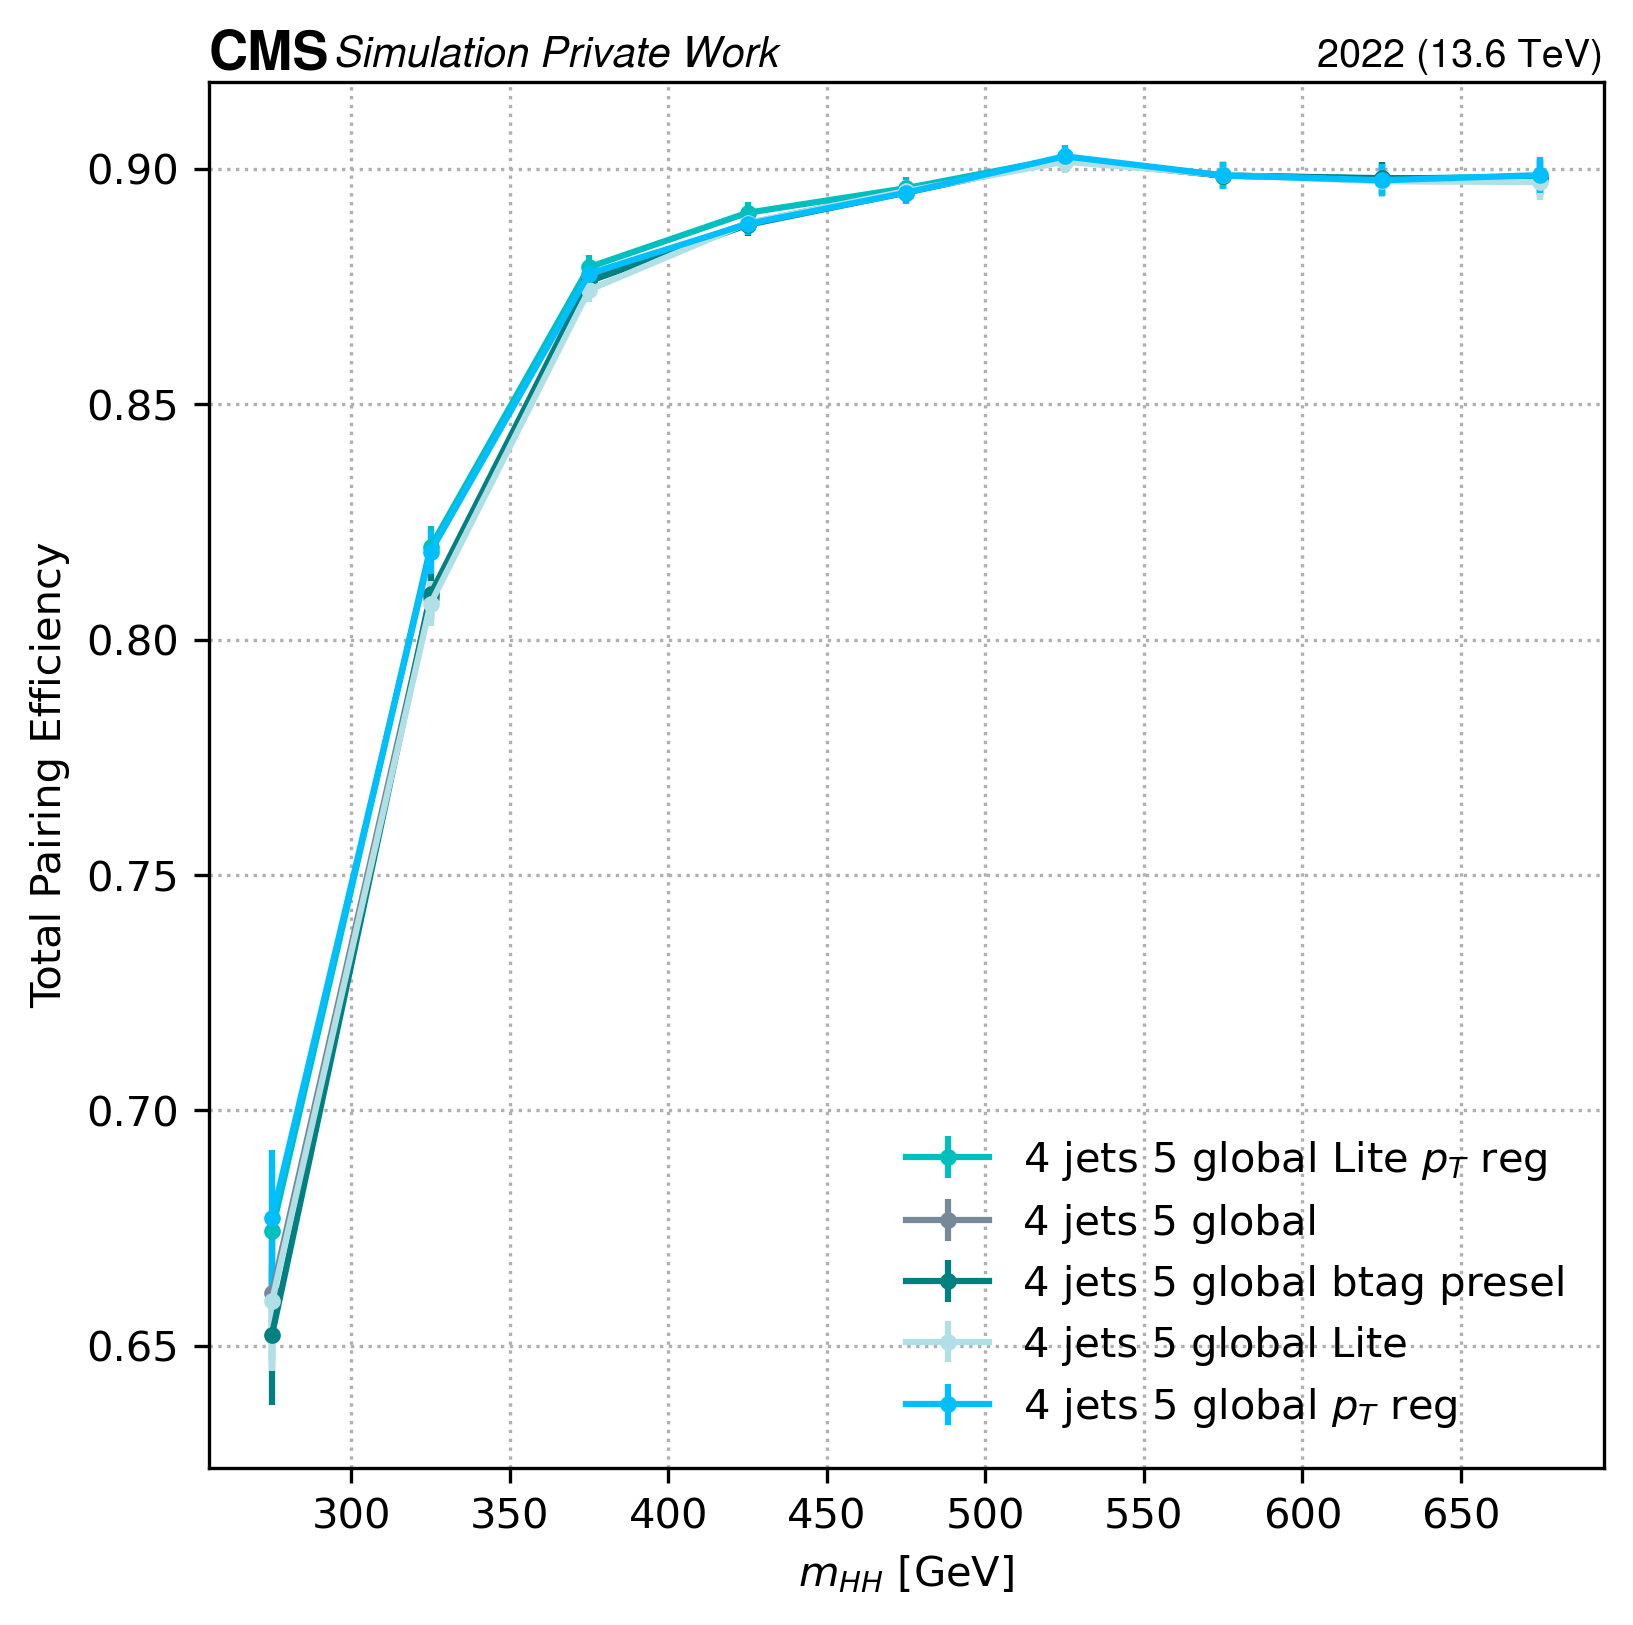
\includegraphics[width=0.6\linewidth]{Images/6.Improving/Imput Comparisons/4j5g training comp.png}
    \caption{Comparison of the total pairing efficiency as a function of $m_{HH}$ for the different trainings presented in Table \ref{table:4 jets trainings} using 4 jets and a 5$^\text{th}$ global as input.}
    \label{fig: comp 4j5g}
\end{figure}

\begin{figure}[h!]
    \centering
    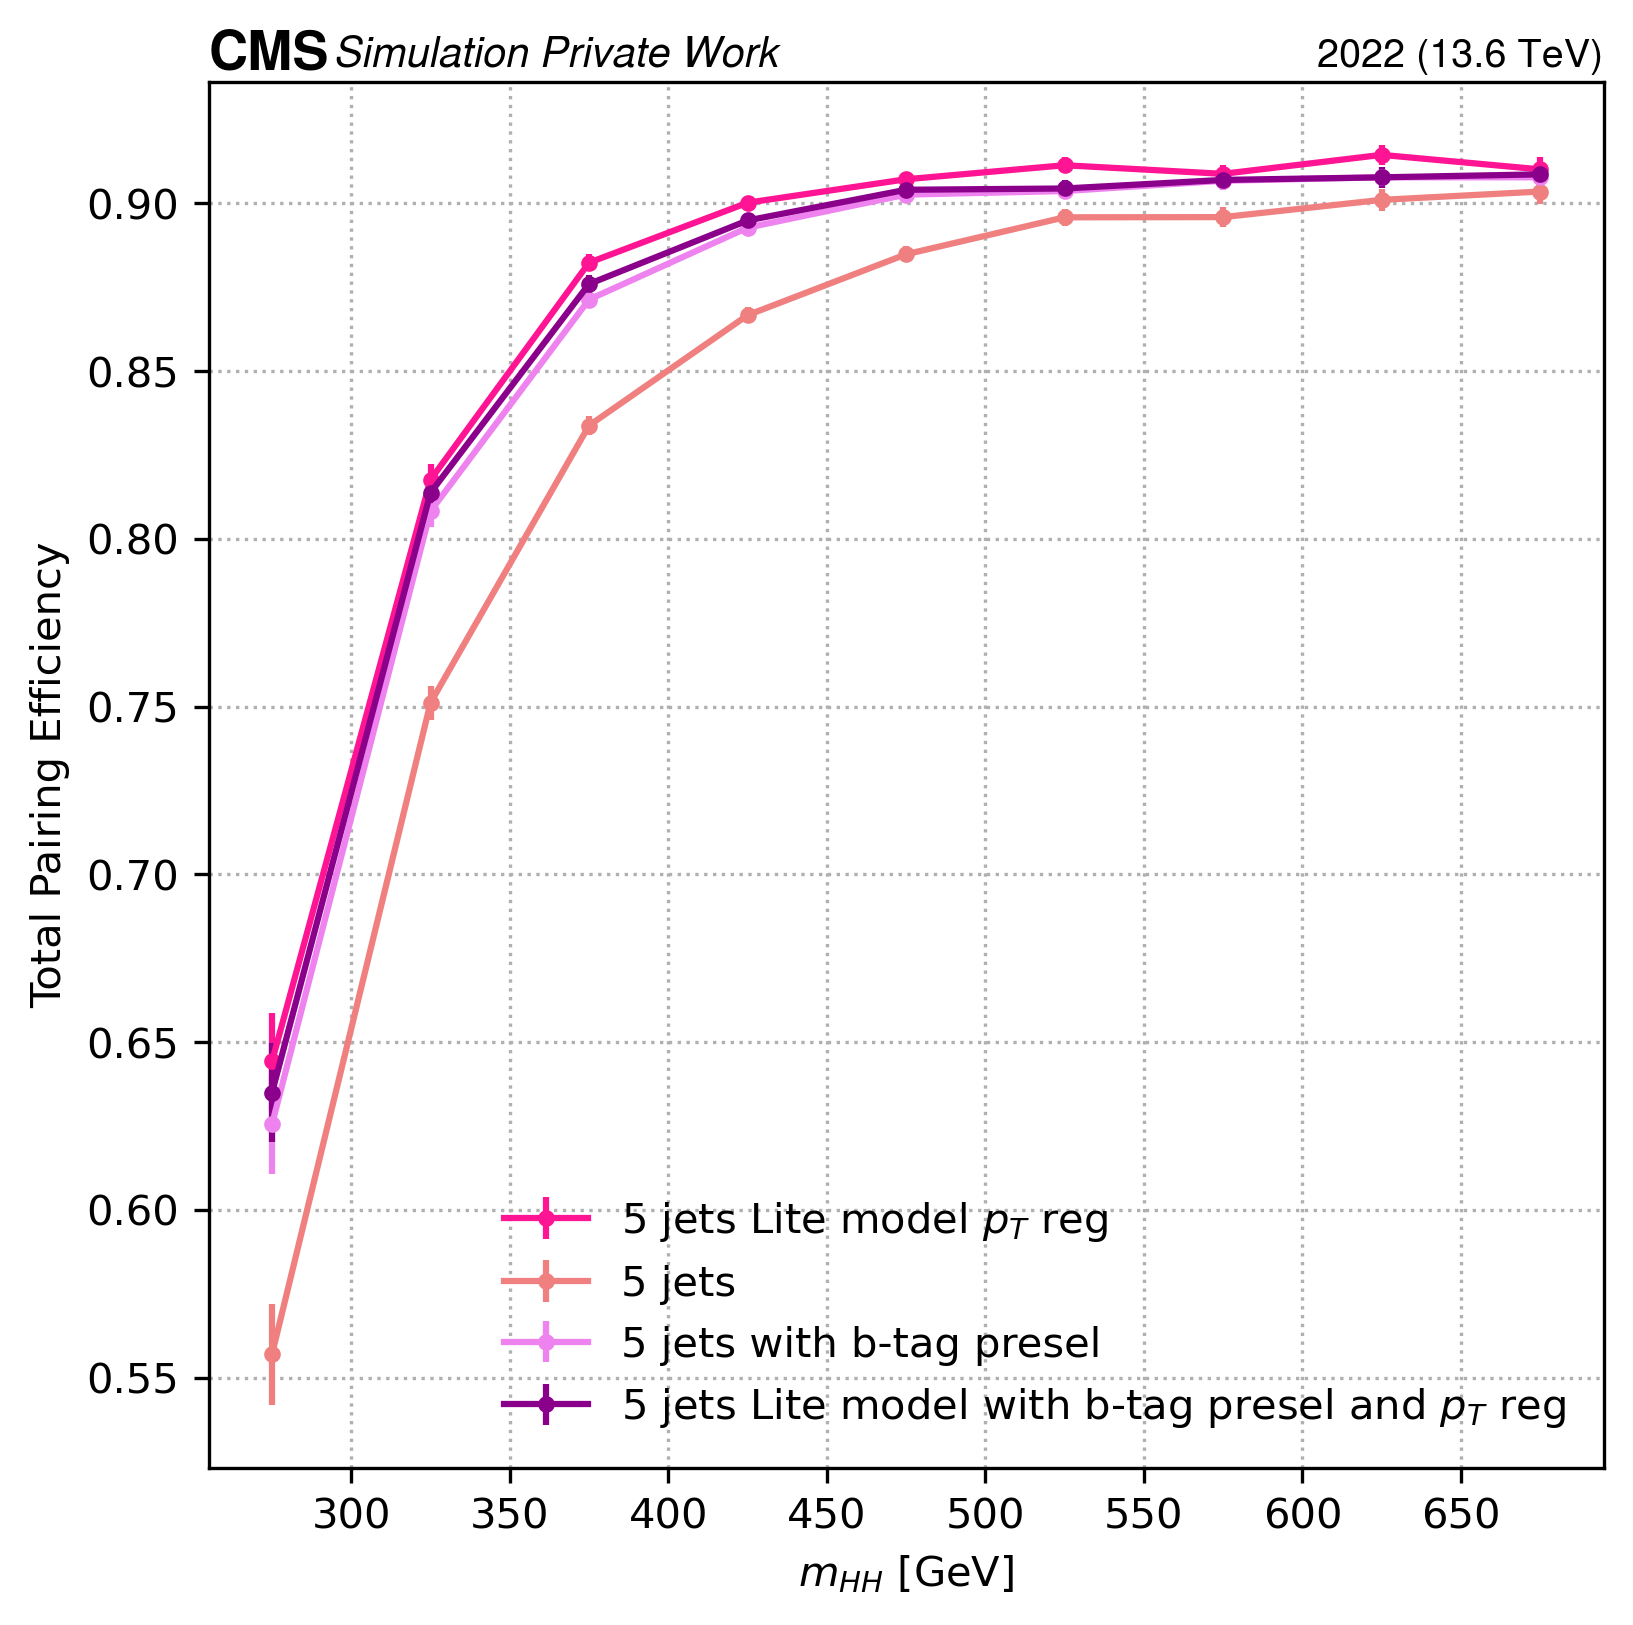
\includegraphics[width=0.6\linewidth]{Images/6.Improving/Imput Comparisons/5j training comp.png}
    \caption{Comparison of the total pairing efficiency as a function of $m_{HH}$ for the different trainings presented in Table \ref{table:5 jets trainings} using 5 jets as inputs}
    \label{fig: comp 5j}
\end{figure}



The next step is to compare these two models to the performance of the previous $D_{HH}$-method presented in section \ref{section: HH4b}. The comparison is performed for events for which we have $\Delta D_{HH} > 30$ GeV, as we only implemented this method for these events. In Figure \ref{fig: 2 best models comp} we show that the 2 models outperform the $D_{HH}$-method. 

\begin{figure}[h!]
    \centering
    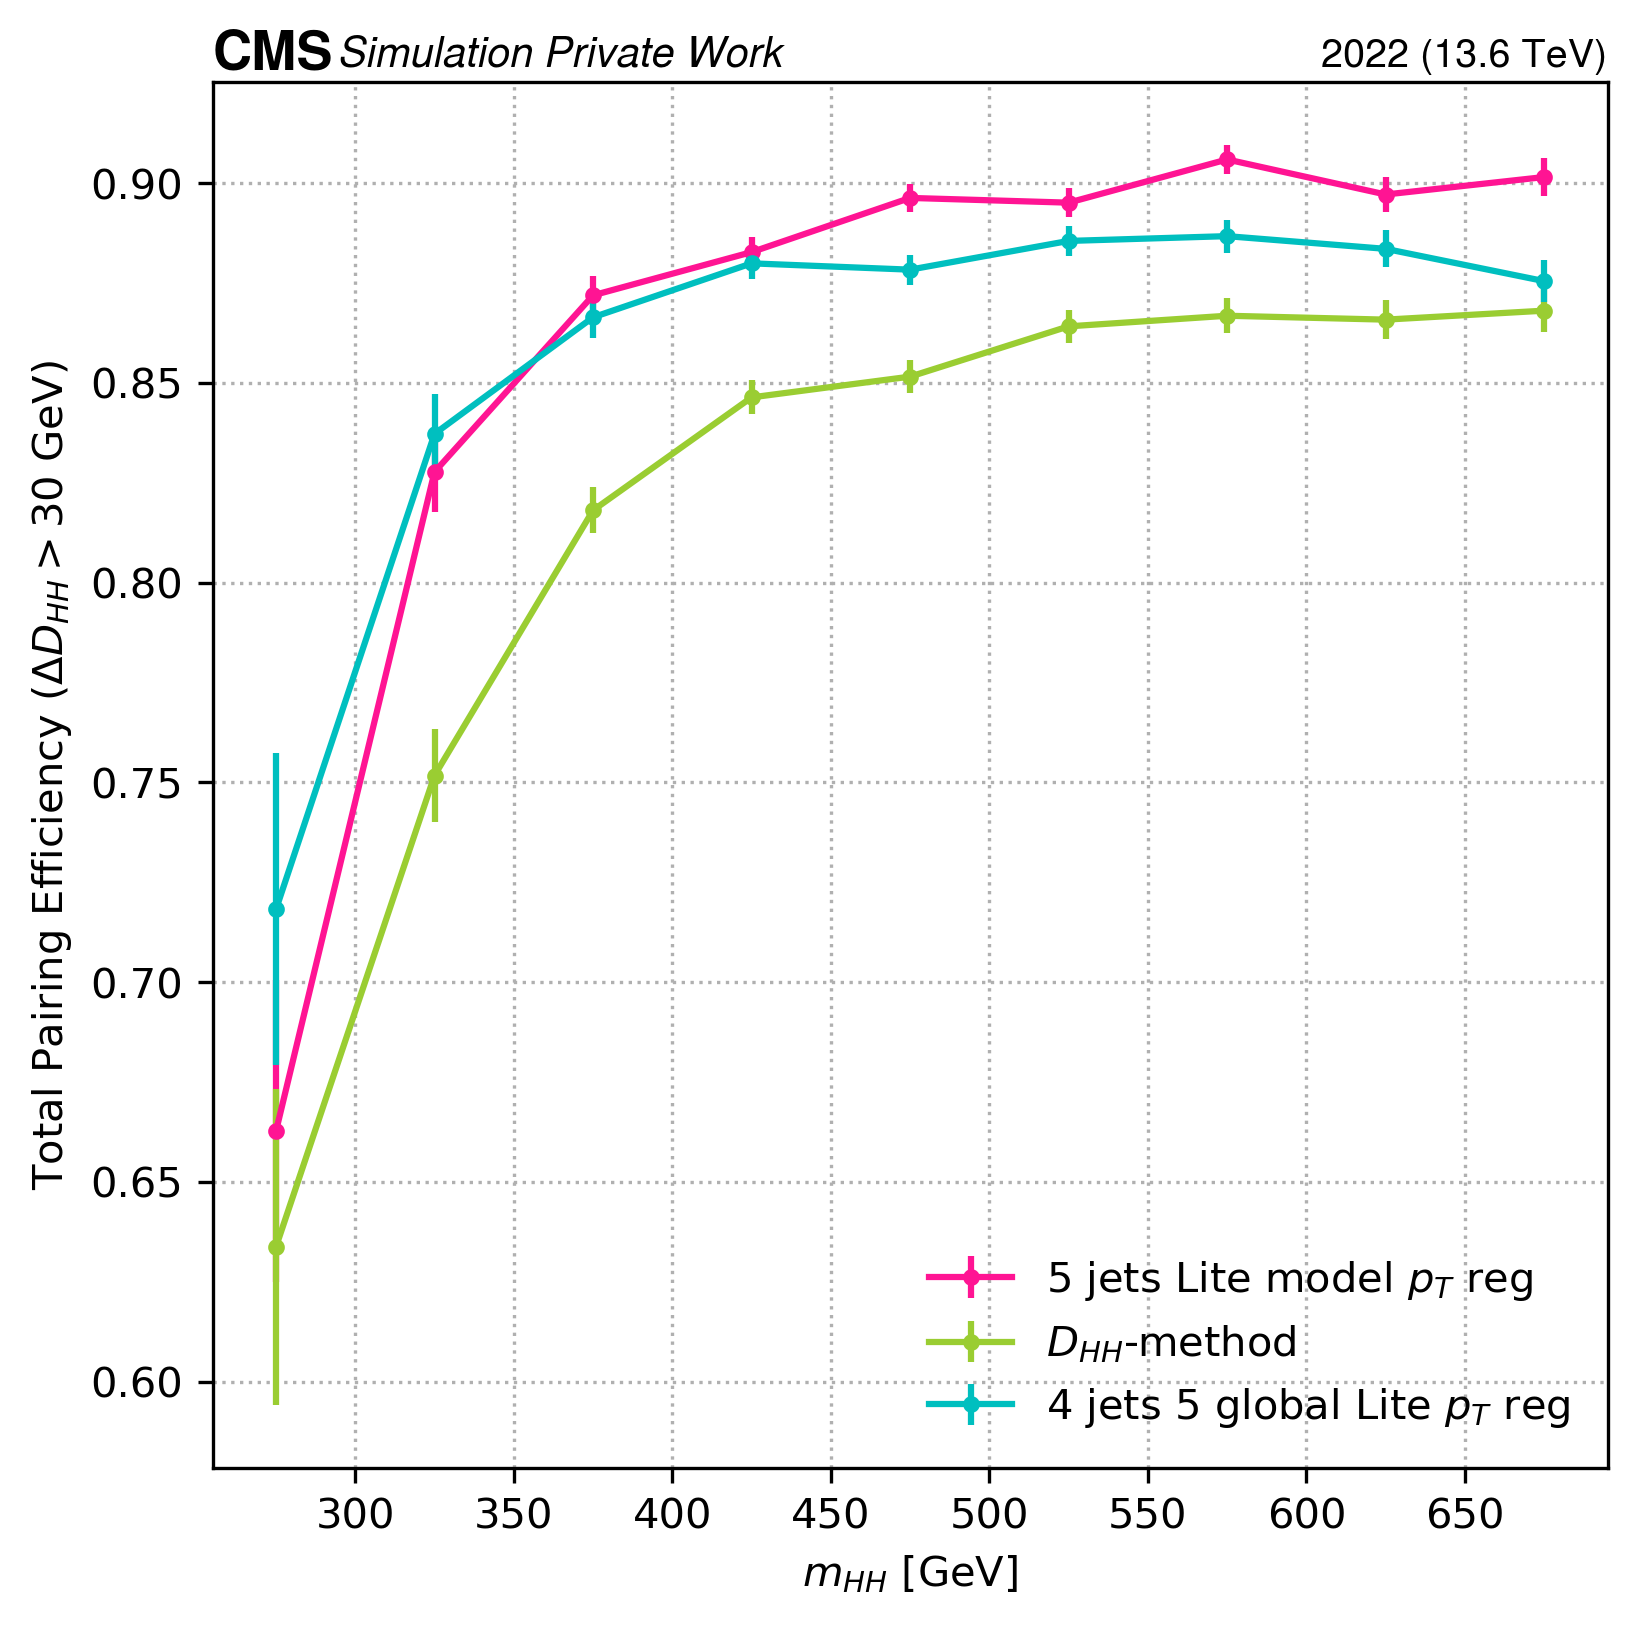
\includegraphics[width=0.6\linewidth]{Images/6.Improving/Imput Comparisons/2 best models comp run2 .png}
    \caption{Comparison of the total pairing efficiency for events where $\Delta D_{HH} > 30$. We compare the performance of the 5 jets Lite model \pt reg defined in Table \ref{table:5 jets trainings} and 4 jets 5 global Lite model \pt reg defined in  Table \ref{table:4 jets trainings}. These are two most performing models we have obtained and we want to compare them here to the performance of the $D_{HH}$-method described in section \ref{section: HH4b} that was used for the pairing in Run 2 }
    \label{fig: 2 best models comp}
\end{figure}


\clearpage

\noindent In conclusion, we converged on two optimized pairing models:

\begin{itemize} [itemsep=0.1em]
    \item 4 jets as sequential inputs with a 5th global jet using the \pt reg $\eta, \phi$ and btag of the jets as well as the Lite model
    \item 5 jets as sequential inputs using the \pt reg $\eta, \phi$ and btag of the jets as well as the Lite model
\end{itemize}

\noindent which have the highest total efficiency and that outperform the pairing efficiency used in the $D_{HH}$-method.

We also tried to asses the performance of these two trainings evaluated on datasets where we only have 4 jets, but these evaluations are not valid due to the difference of phase space, i.e. the jet multiplicity and all observables correlated to it, between the train and the test files.  

Lastly, we wanted to perform a training without the b-tag of the jet because this observable is already used in the DNN for the 2b to 4b morphing for the QCD background estimation (described in \ref{section: HH4b}). Therefore, if we use b-tag in our training and evaluate our model in the 4b morphed data, there could be some correlations due to the fact that this variable is used for both networks. Nevertheless, the performance was observed to be worse than by including it in the inputs. If we compare the validation accuracy (defined in section \ref{section: spanet architecture}) when training the network without b-tag using the 5 jets Lite model \pt reg model we have a validation accuracy of 0.875 compared to 0.968 when taking b-tag as input. We conclude that for the following section we will use b-tag as input variable in the trainings where we use SPANet for the pairing.

\clearpage

\subsection{Background mass sculpting} \label{subsection: bckg mass sculpting}
In addition to the pairing efficiency, another figure of merit used in order to select the best model is the mass sculpting of the background.  Even though the training using 5 jets as inputs outperforms the training using 4 jets with a 5$^{\text{th}}$ global in terms of total pairing efficiency, we want to verify if when evaluating these models on background events we do not observe a fake peak of events around the SR ( defined in Section \ref{section: HH4b}). 

To verify this, we will use the models we presented in the last section and evaluate them in a sample of 2b data defined in Section \ref{section: HH4b}. Moreover, as explained in Section \ref{subsection:cutflows} due to the requirements of the 2b region, we have mostly background events and the signal contribution due to the mistagging of the jets is negligible. Hence, if we evaluate our model on the 2b data sample, we should not observe a peak of events in the $m_{HH}$ plane around the signal region (defined in section \ref{section: HH4b}). In Figure \ref{fig: 2D mass dist sig}, we show the 2D mass distribution of the evaluation of our model on signal events. We can observe that most of the predicted events are in the signal region. On the contrary, in Figures \ref{fig: 2D mass sculpting for 4j5g} and \ref{fig: 2D mass sculpting for 5j}, we show the 2D mass distributions of the evaluation of the two best models described in Section \ref{subsection: choice of inputs} on 2b data. We observe that there is not a peak of events in the signal region, which shows that the SPANet pairing algorithm is not affected by the mass sculpting. 

\begin{figure}[hbt]
    \centering
    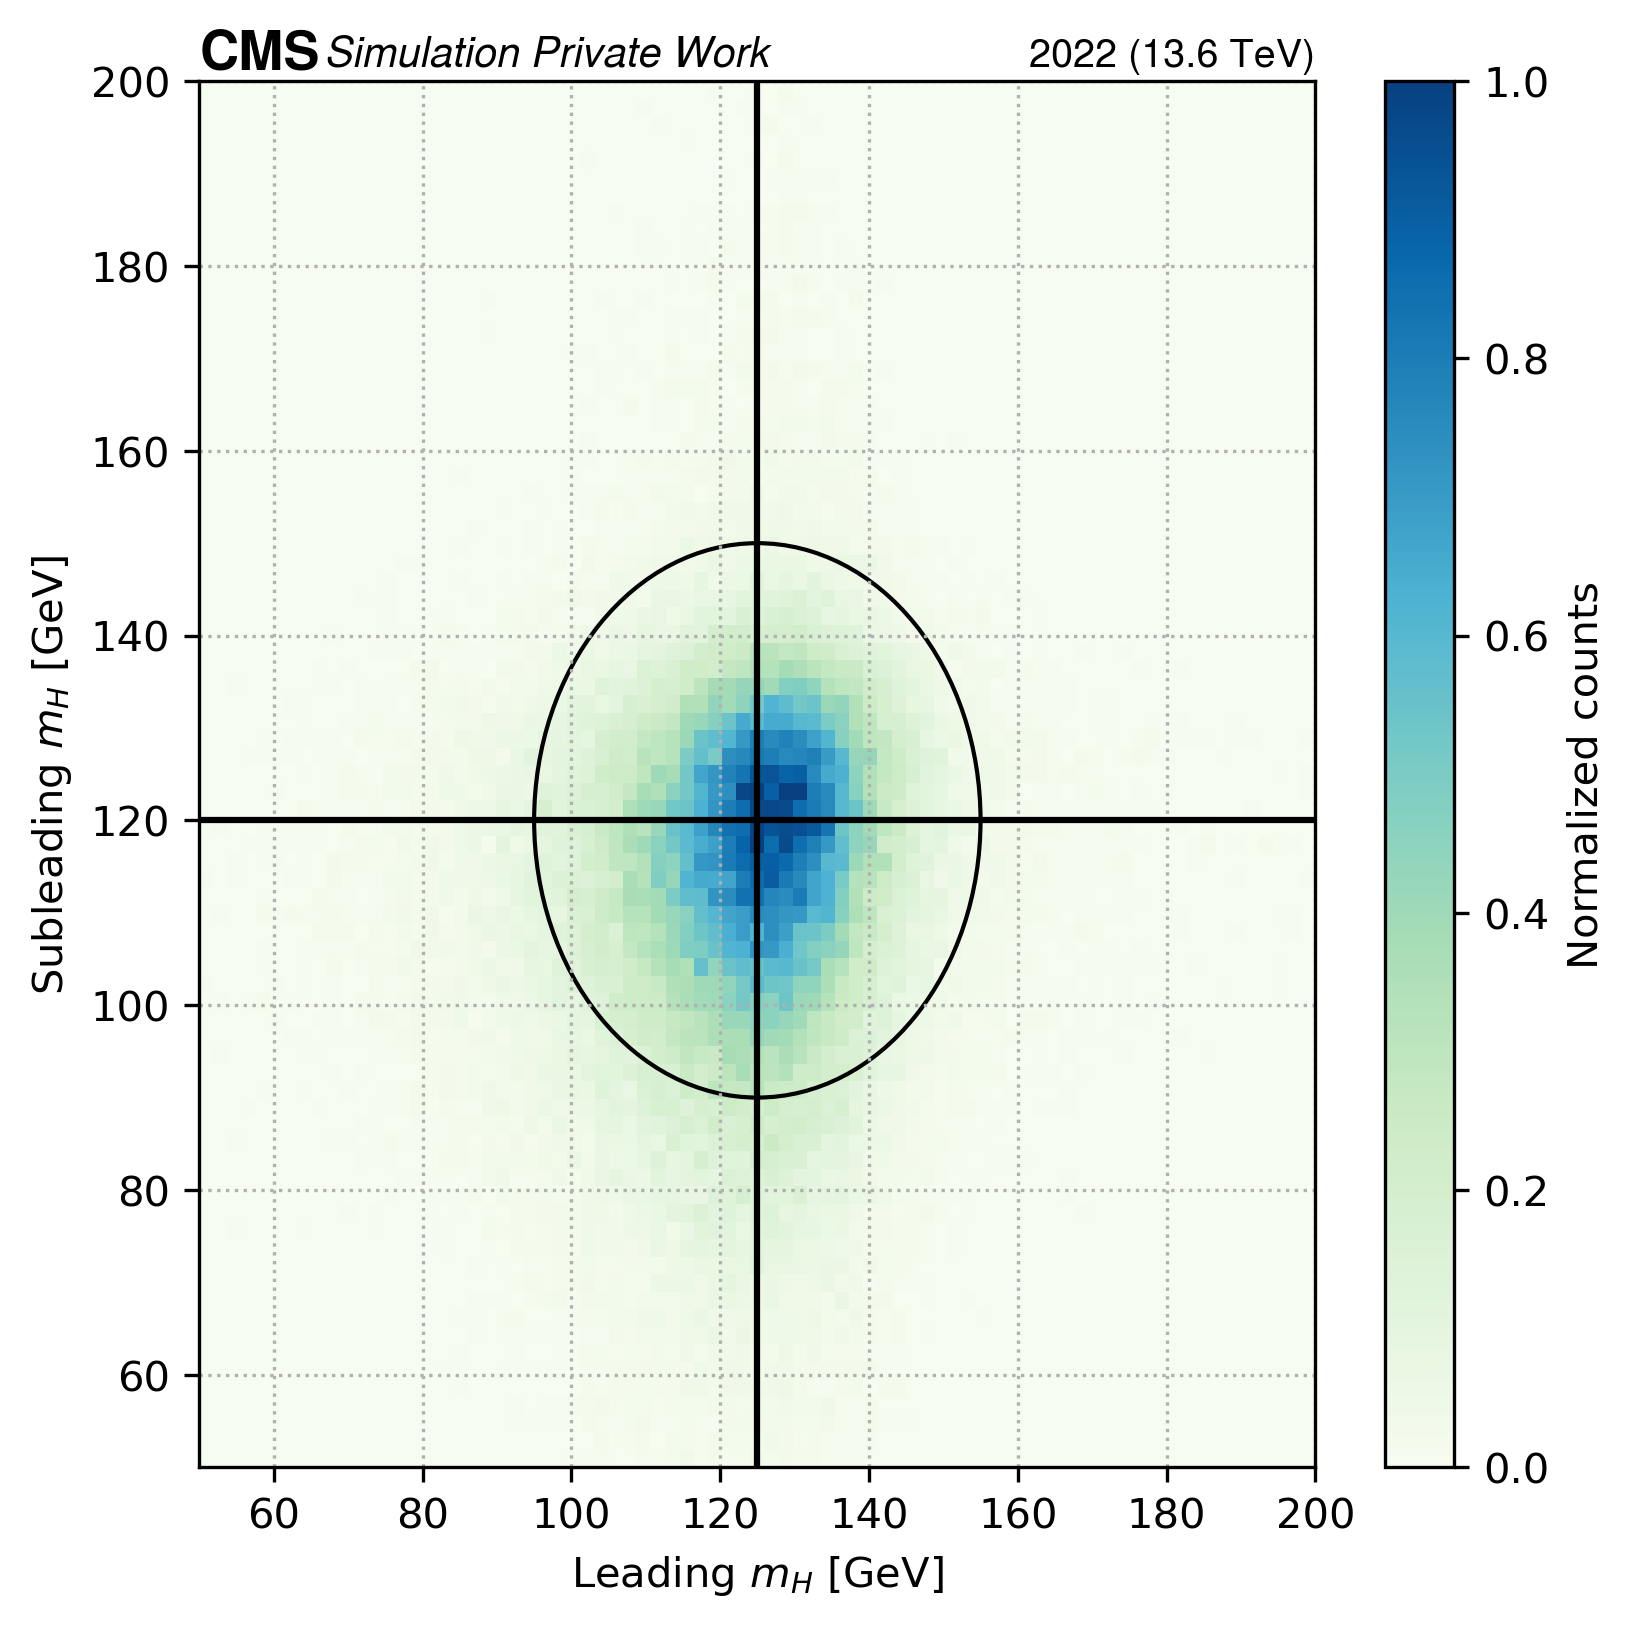
\includegraphics[width=0.6\linewidth]{Images/6.Improving/Mass sculpting/signal mhh.png}
    \caption{Higgs mass distribution of the leading Higgs on the x-axes and the subleading Higgs on the y-axes after the evaluation of the 4 jets 5$^{\text{th}}$ jet model on signal events. The vertical black line corresponds to the mass of the leading Higgs and the horizontal of the subleading Higgs. The black circle defines the SR area defined in Section \ref{section: HH4b}}
    \label{fig: 2D mass dist sig}
\end{figure}


\begin{figure}[hbt]
    \centering
    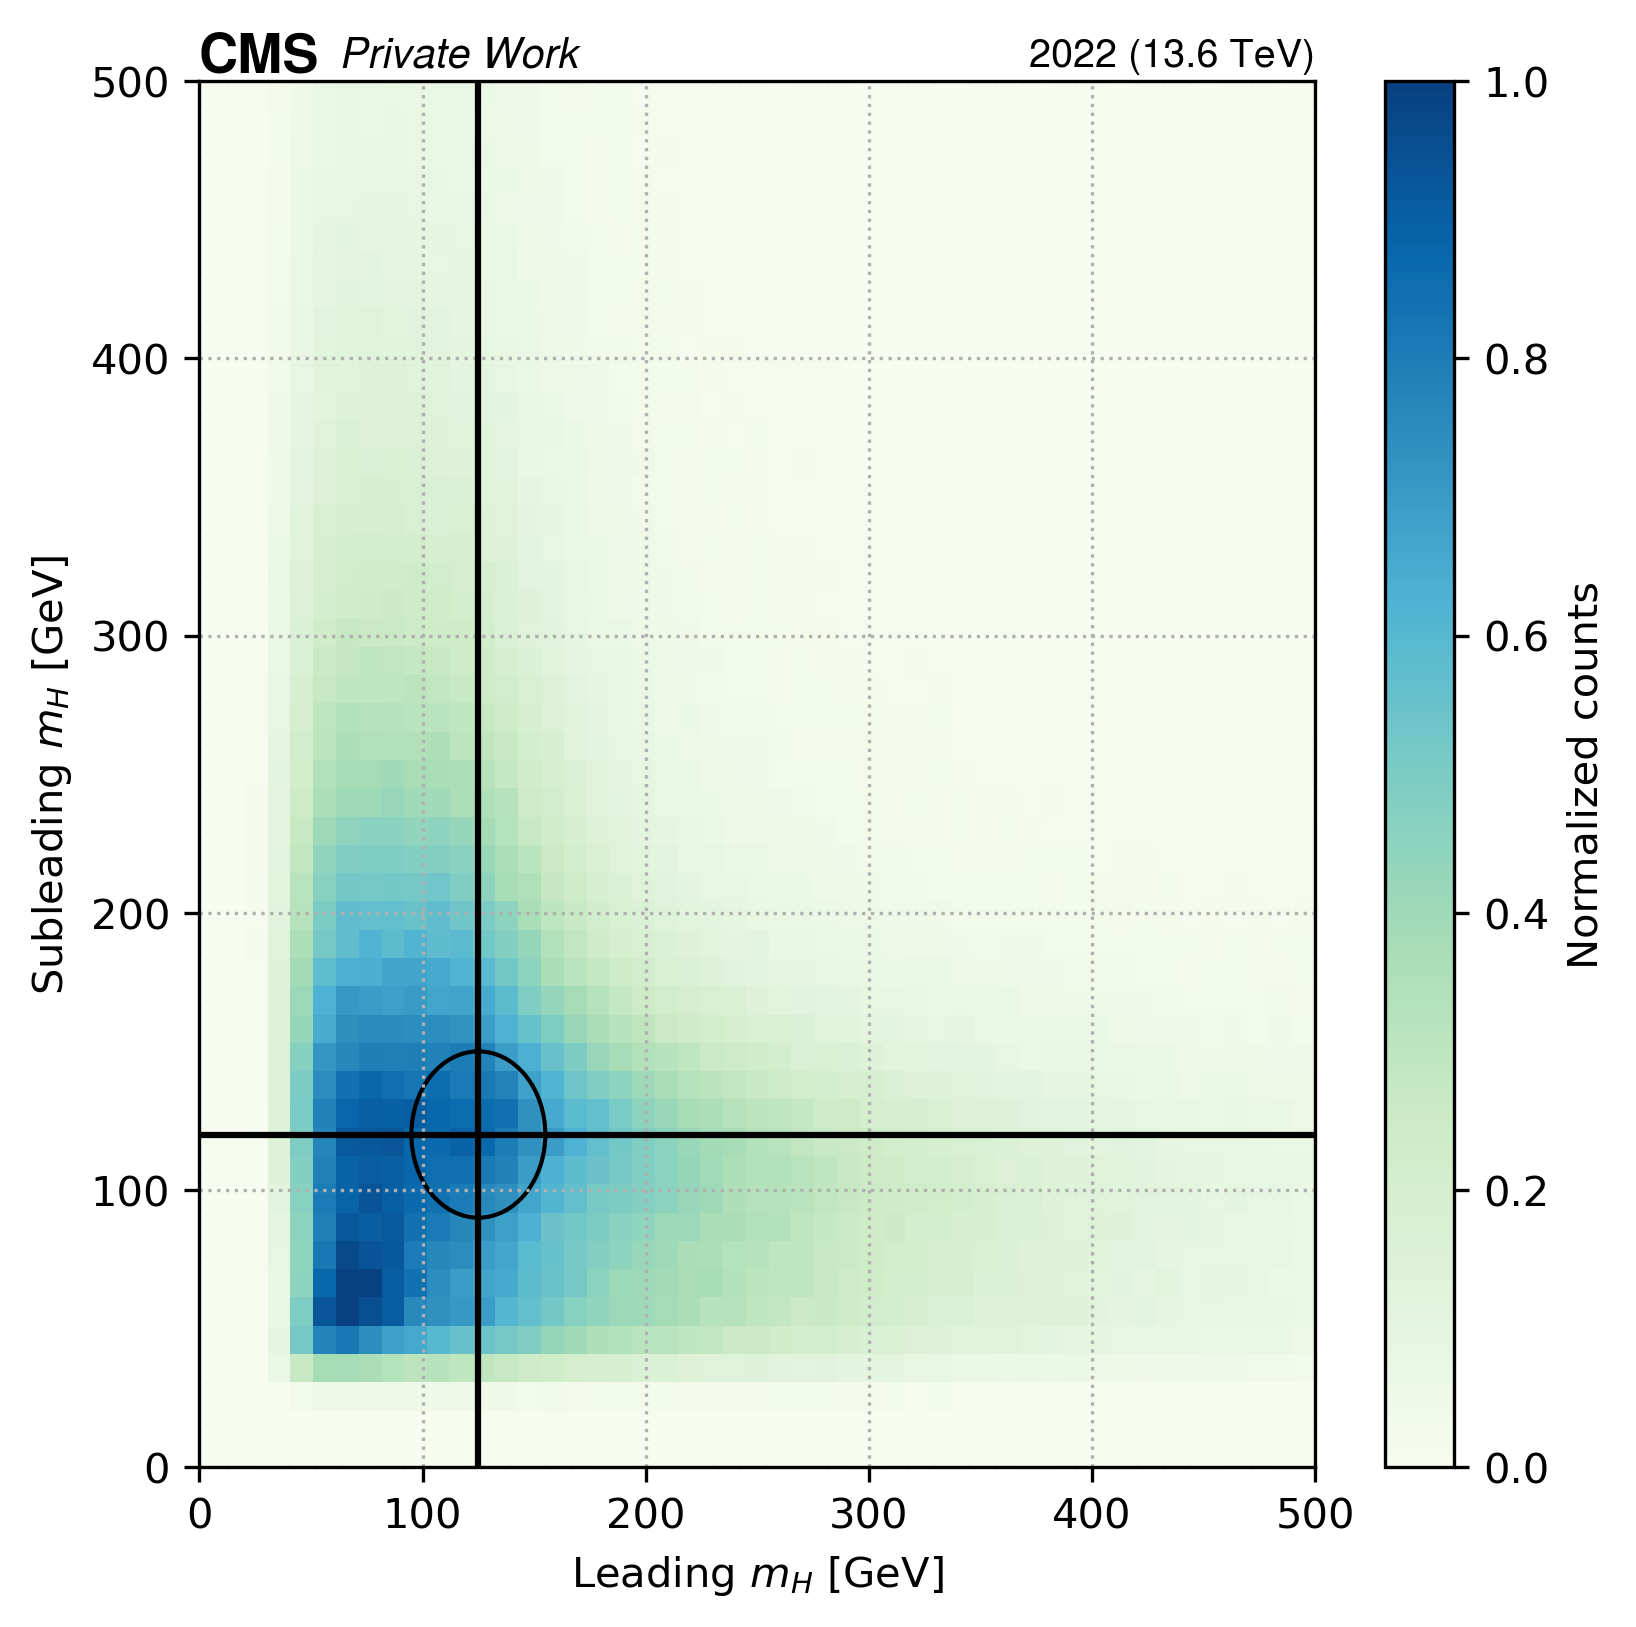
\includegraphics[width=0.6\linewidth]{Images/6.Improving/Mass sculpting/mass sculpting 4j5g.png}
    \caption{Higgs mass distribution of the leading Higgs on the x-axes and the subleading Higgs on the y-axes after the evaluation of the 4 jets 5$^{\text{th}}$ jet model on 2b data. The vertical black line corresponds to the mass of the leading Higgs and the horizontal of the subleading Higgs. The black circle defines the SR area defined in Section \ref{section: HH4b}}
    \label{fig: 2D mass sculpting for 4j5g}
\end{figure}



\begin{figure}[hbt]
    \centering
    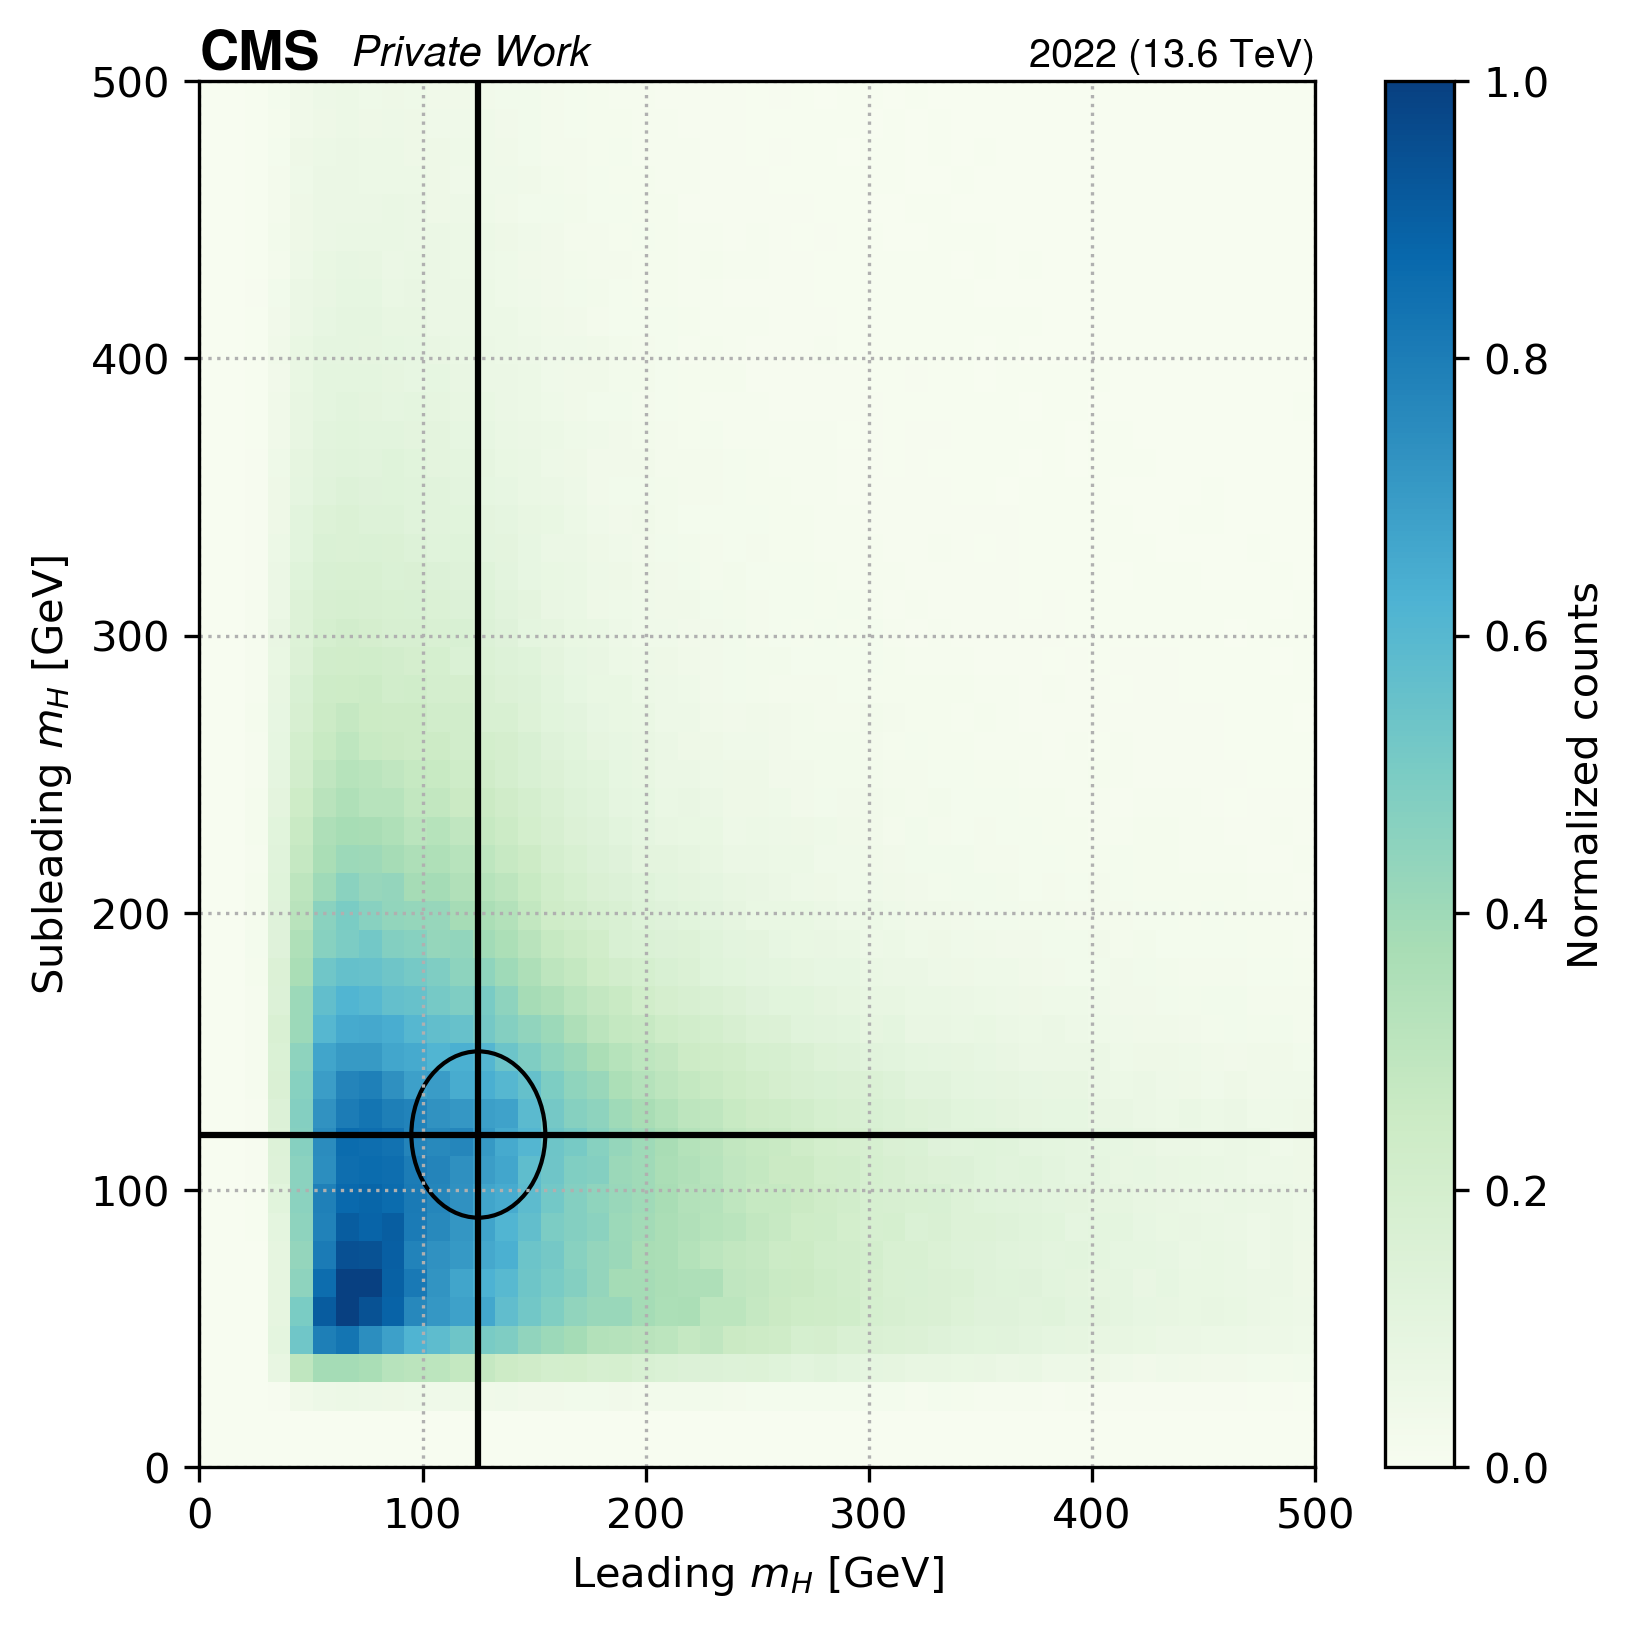
\includegraphics[width=0.6\linewidth]{Images/6.Improving/Mass sculpting/mass sculptimg 5j.png}
    \caption{Higgs mass distribution of the leading Higgs on the x-axes and the subleading Higgs on the y-axes after the evaluation of the 5 jet model on 2b data. The vertical black line corresponds to the mass of the leading Higgs and the horizontal of the subleading Higgs. The black circle defines the SR area defined in Section \ref{section: HH4b}}
    \label{fig: 2D mass sculpting for 5j}
\end{figure}


In Figures \ref{fig: 1D mass sculpting leading} and \ref{fig: 1D mass sculpting subleading} the comparison of the mass sculpting for the leading and the subleading Higgs respectively in the 1D plane is shown. In these plots we can compare the two models and conclude that there is less sculpting when considering the training with 5 jets, for both the leading and the subleading Higgs. Therefore, the model where we give 5 jets as inputs, with \pt reg and using the Lite hyperparameters not only has the best pairing efficiency but also the mass sculpting is smaller than with the 4 jets model. Therefore, in the following sections, we will use this model.

\begin{figure}[hbt]
    \centering
    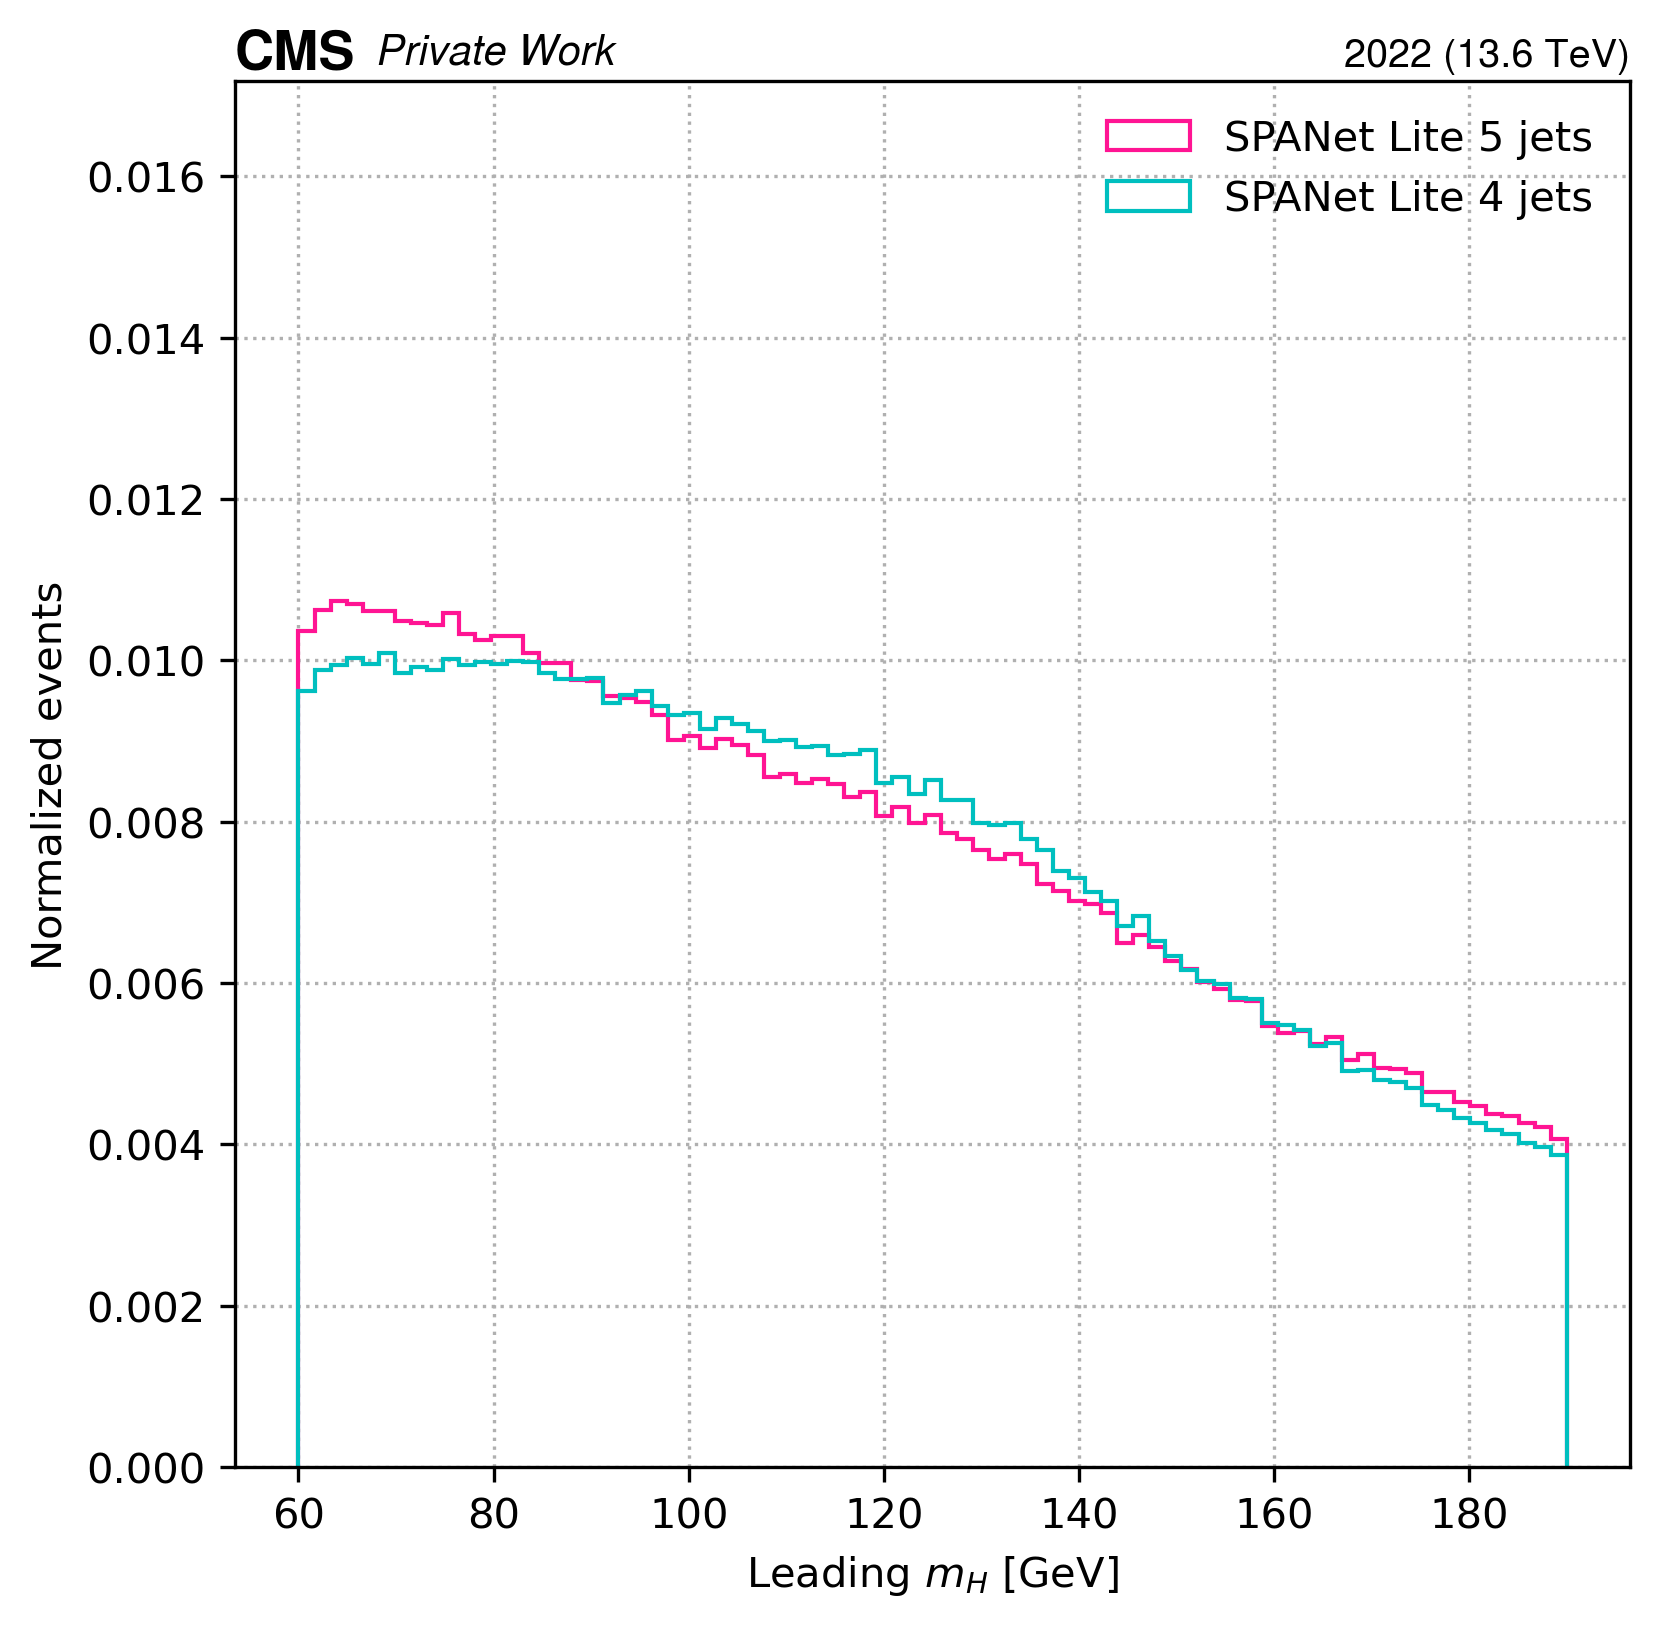
\includegraphics[width=0.6\linewidth]{Images/6.Improving/Mass sculpting/lead h sculpting.png}
    \caption{Distribution of the leading Higgs mass after the evaluation of the best performing models defined in Section \ref{subsection: results on the trainings} on 2b data}
    \label{fig: 1D mass sculpting leading}
\end{figure}

\begin{figure}[hbt]
    \centering
    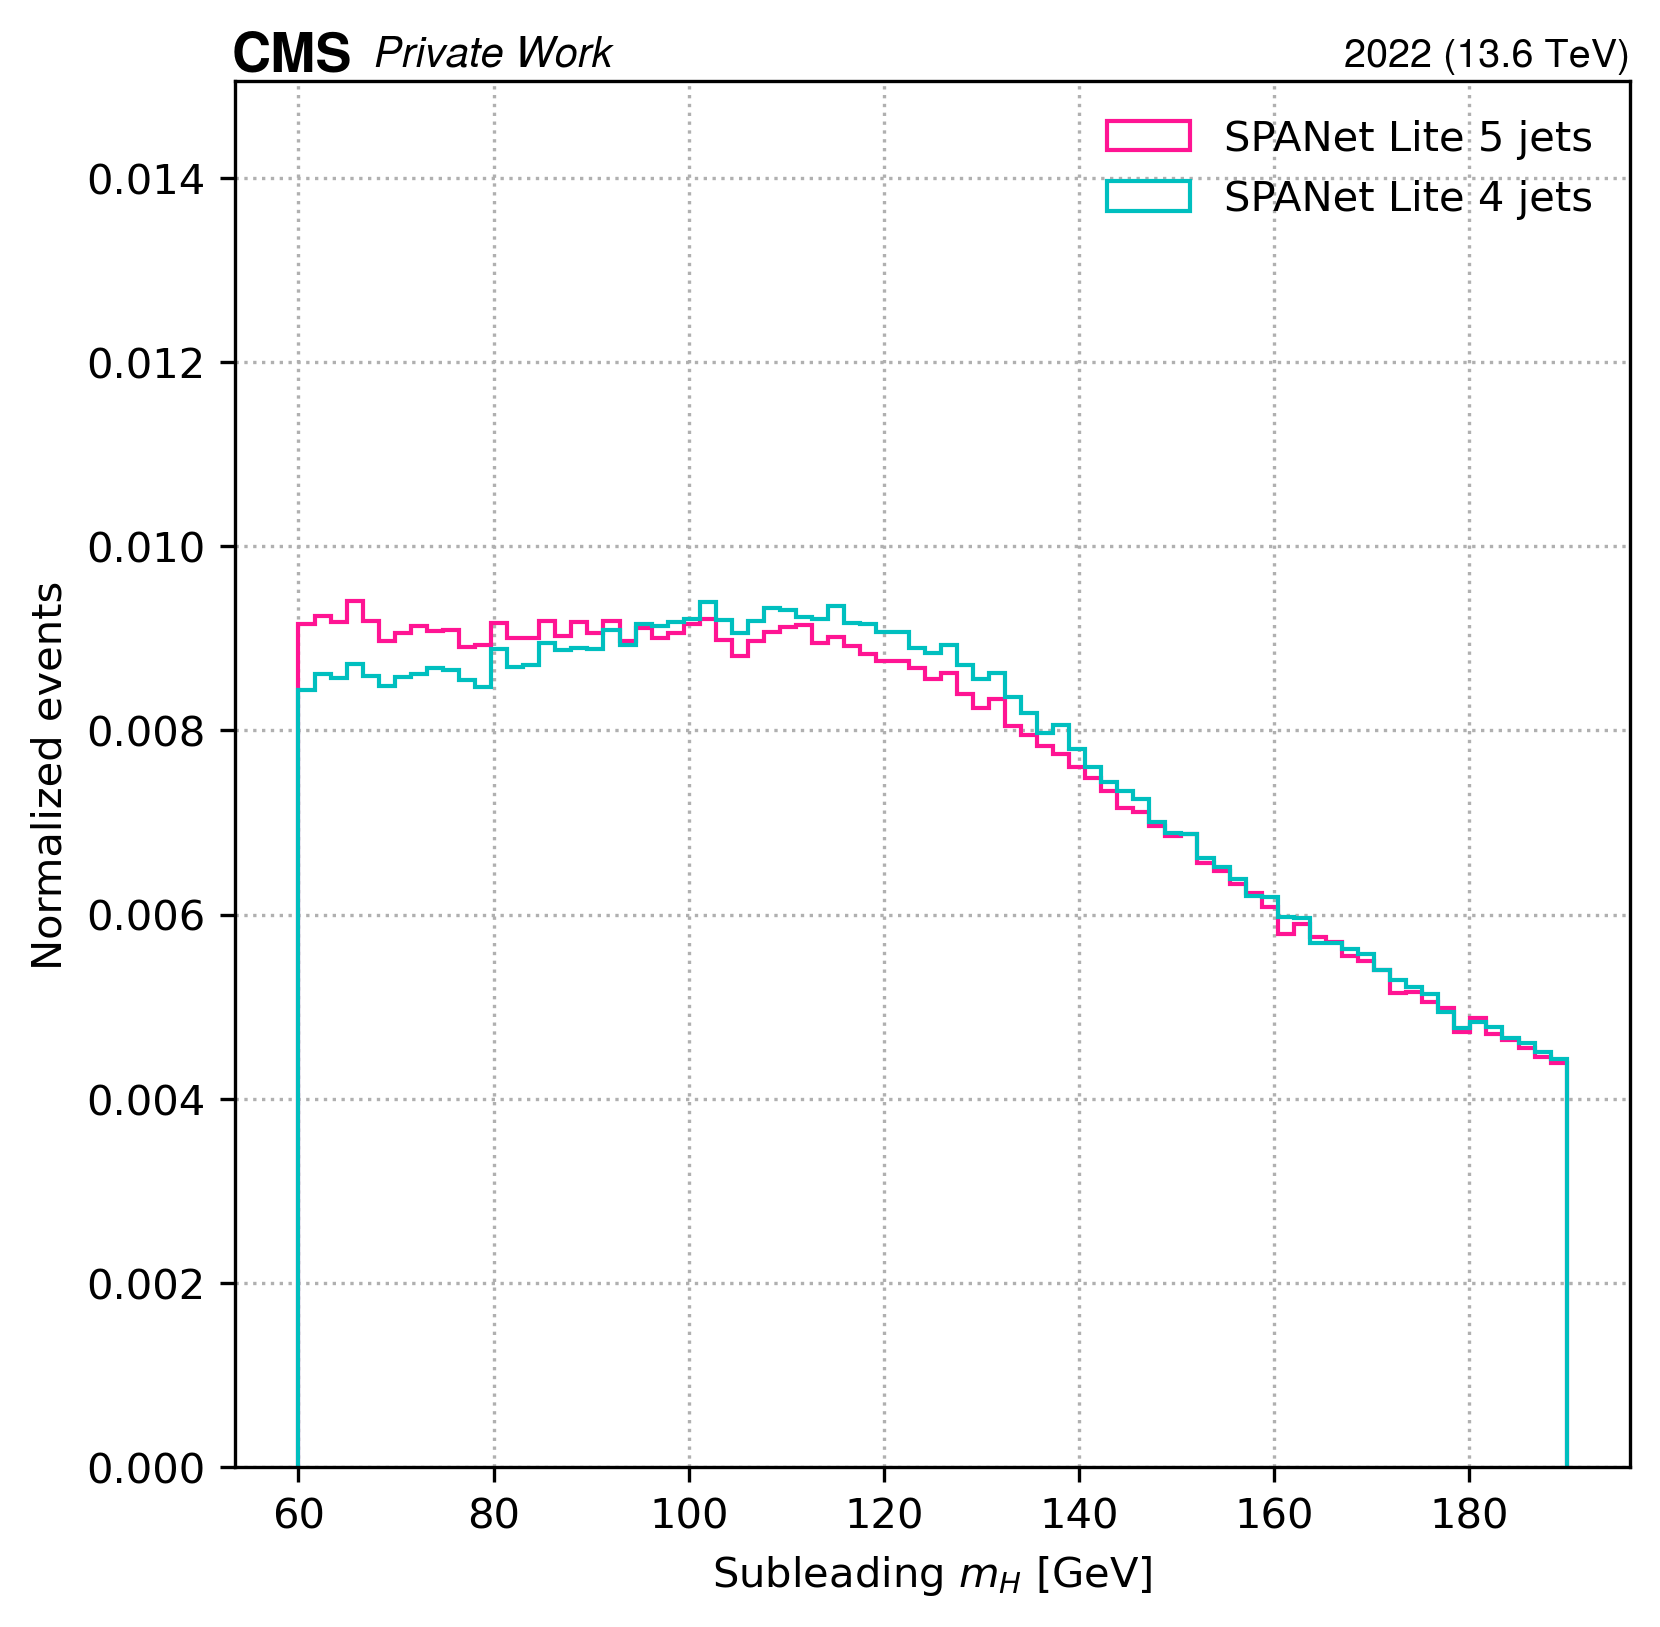
\includegraphics[width=0.6\linewidth]{Images/6.Improving/Mass sculpting/subleading h sculpting.png}
    \caption{Distribution of the subleading Higgs mass after the evaluation of the best performing models defined in Section \ref{subsection: results on the trainings} on 2b data}
    \label{fig: 1D mass sculpting subleading}
\end{figure}

%The next question that arises when performing these tests, is that after performing several trainings with 5 jets, we observed a variability in the results, which is why, we decided to delve onto the variability of these trainings.

\clearpage

\subsection{Studies for the SPANet training variability} \label{subsection: pairing variability}

After performing several trainings with 5 jets, we observed a variability in the results, which is why, we decided to delve onto the "model variability" of these trainings. We define the "model variability" that will be tested in this section as the variability of our training with respect to the validation accuracy defined in section \ref{section: spanet architecture}.

In order to asses the model variability, we performed several trainings of the same model fixing the seed to randomly initialize the weights. As a first test to address this variability issue, in addition to fixing the weights, we verified if the Pytorch version used for the training impacted the training variability. We performed 3 different trainings fixing the seeds to 0, 1 and 2 for 3 different versions of Pytorch. We concluded that the variability is independent of the version we use when we fix the seed to initialize the weights, therefore we decided to use the latest version (2.2.2) for our future trainings. Using this version we performed 26 different trainings with 26 different seeds to observe the variability. The results are shown in Figure \ref{fig: 5j variability}, where we show the validation accuracy for each training as a function of the batch size. We observe that the validation accuracy clusters around two different values: 96.6\% and 94.5\%. Around each value we have a spread of around 0.3\%. Therefore, we conclude that there is a large variability of our model ($\sim$2\%). If our model has a validation accuracy of 94.5\% we don't outperform the pairing efficiency of Run 2 anymore. To solve this this, the hyper-parameters of the training are modified in order to mitigate the intrinsic training variability assessed by checking the validation accuracy spread as a function of the batch size

\begin{figure}[hbt]
    \centering
    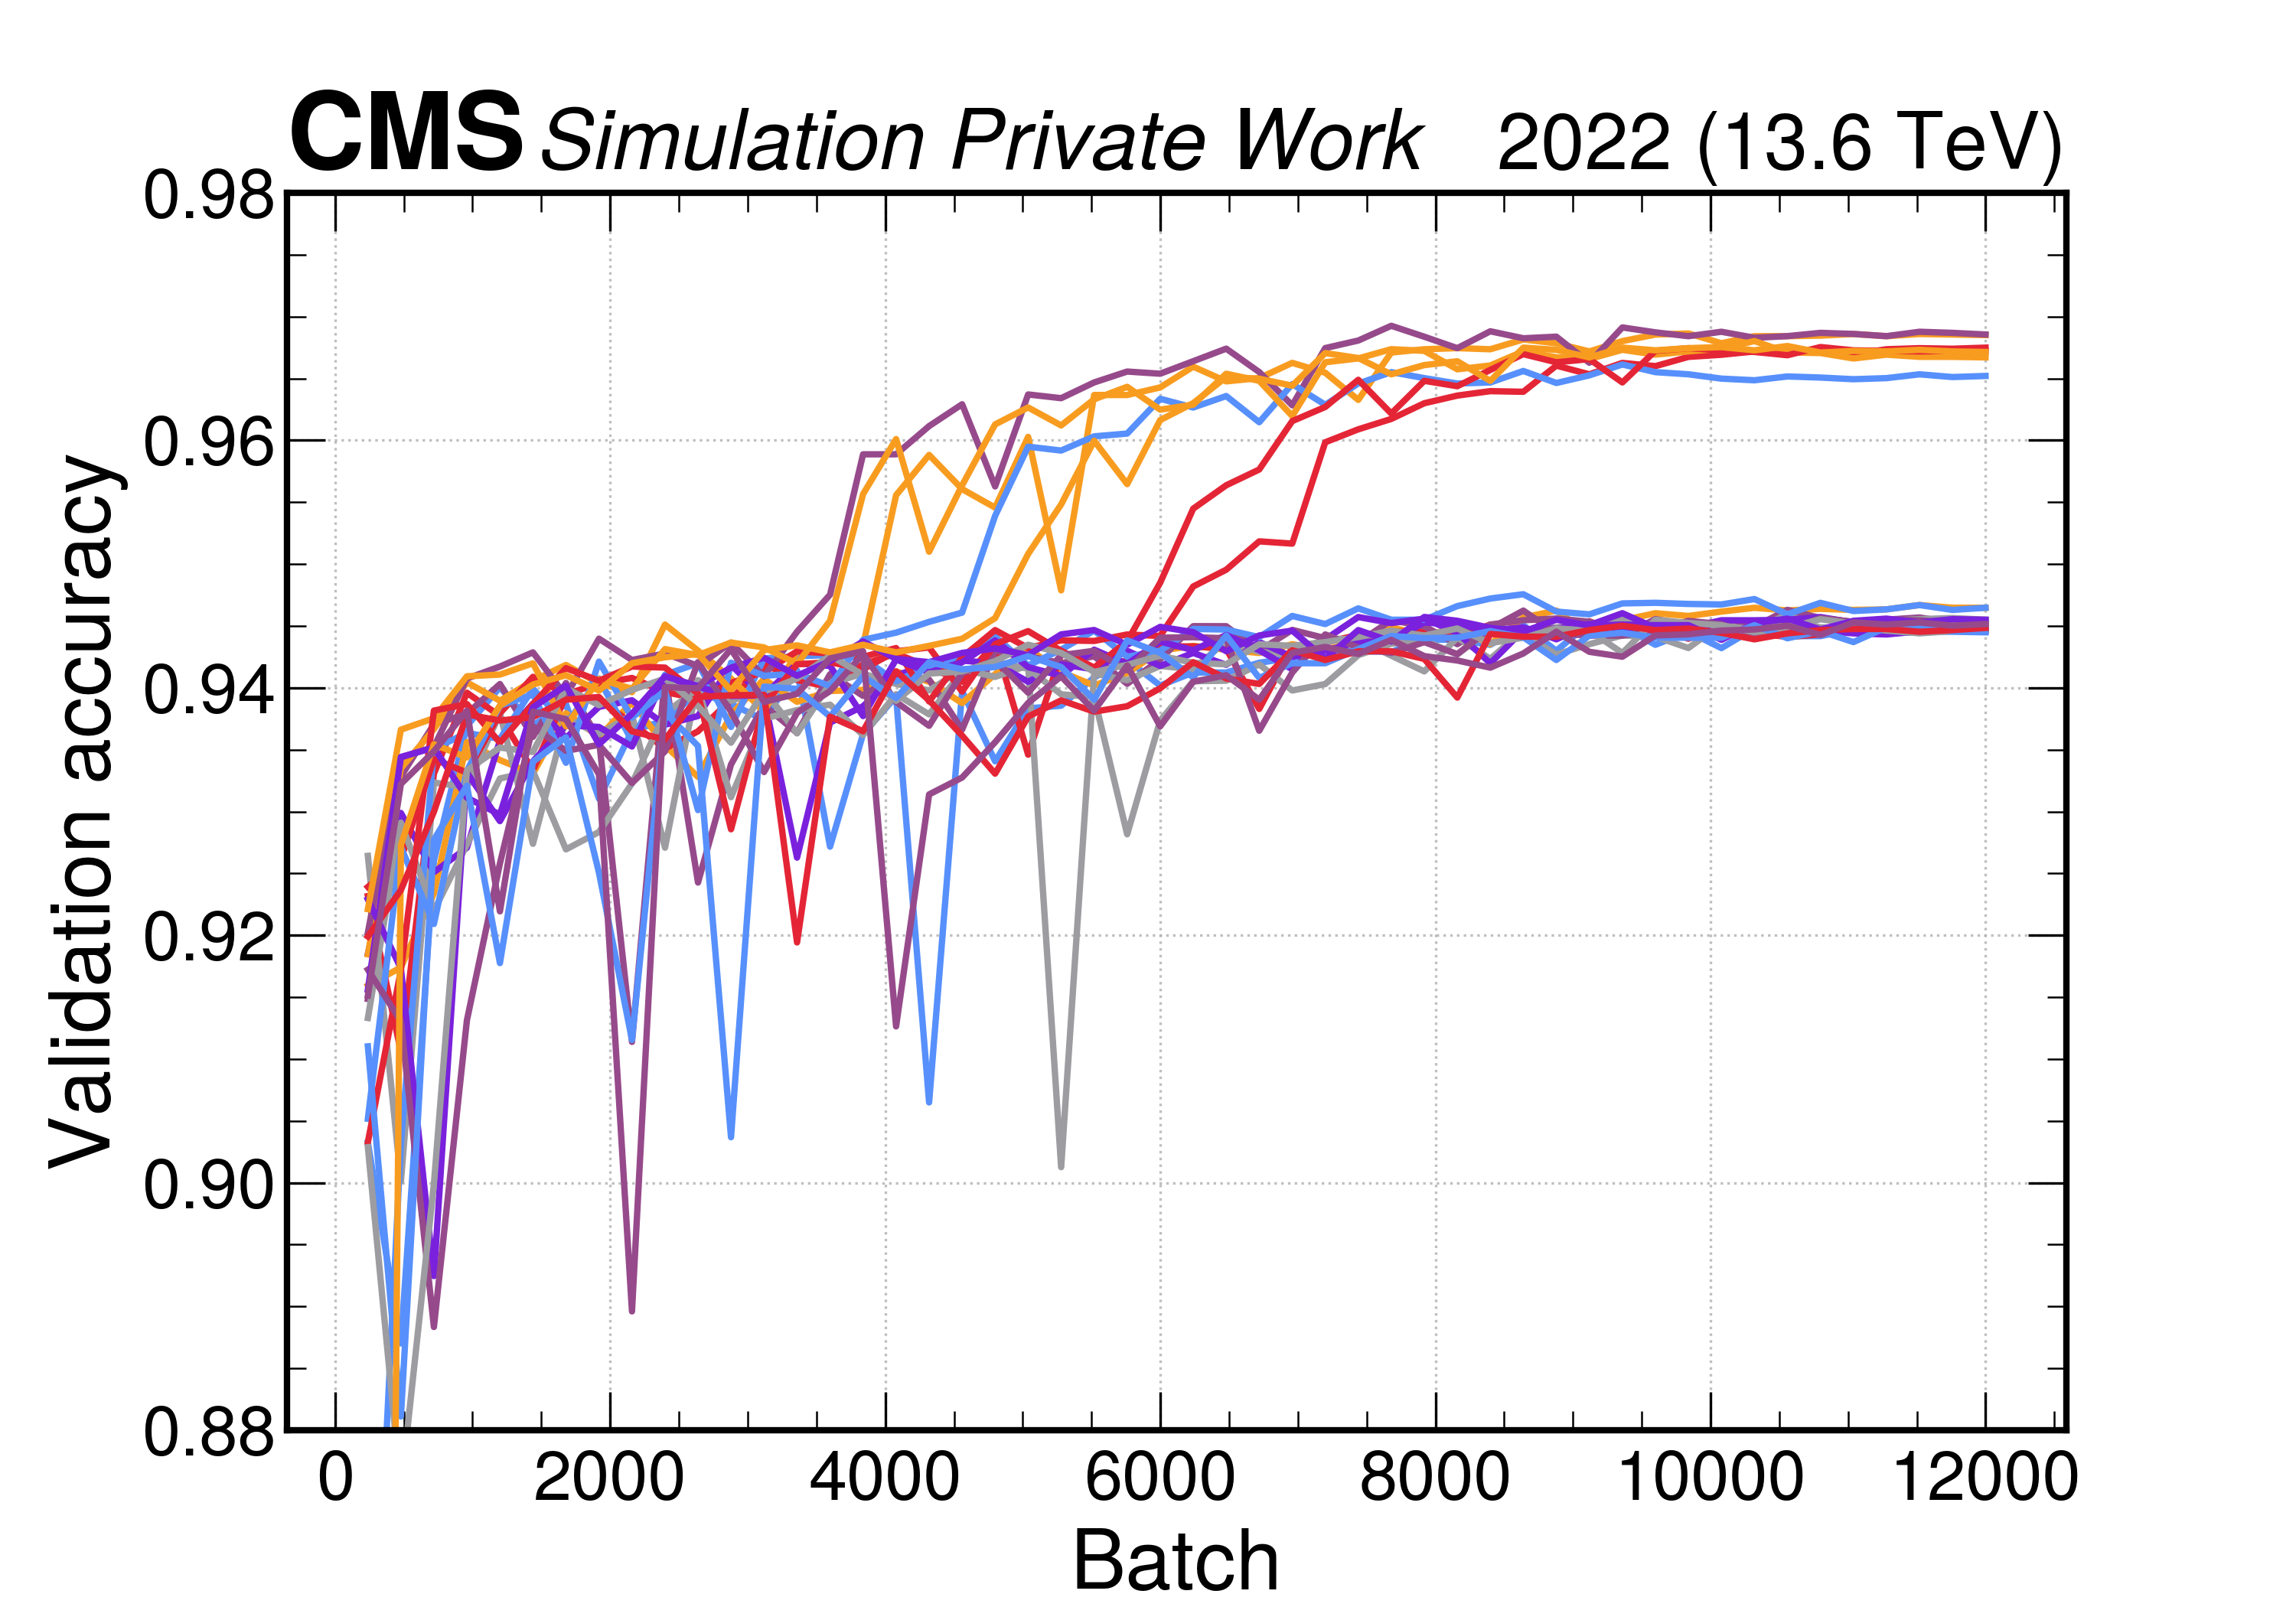
\includegraphics[scale=0.1]{Images/6.Improving/Variability Study/5 jets variability study.png}
    \caption{Variability of the validation accuracy as a function of the batch size of the training using 5 jets as inputs \pt reg and Lite model parameters defined in Table \ref{table:5 jets trainings}}
    \label{fig: 5j variability}
\end{figure}

In Table \ref{table:comparison_models}, the hyper-parameters of the Lite model were defined. Table \ref{table: variation hyperpaparm } shows the parameters of this model we aim to modify to mitigate the variability of our training. We will start by modifying the learning rate. The smaller the learning rate (LR), the more stable the model should be, therefore, we try to decrease the value of the latter. Moreover, by modifying the LR warm-up cycles and rate cycles, instead of reaching the highest values of the learning rate after a few batches as shown in Figure \ref{fig: lr comp}, we start from the highest value and decay linearly. The highest values we will be testing are shown in Table \ref{table: variation hyperpaparm }.

\begin{table}[hbt]
\centering
\begin{tabular}{|p{5cm}|p{4cm}|p{5cm}|}
 \hline
 Hyper-parameters  & Lite model & Test for stabilization \\
 \hline
 Learning rate & 0.00659 & $5\times 10^{-3}$, $10^{-3}$, $5\times 10^{-4}$, $10^{-4}$ \\
 \hline
 Learning rate warmup cycles & 1 & 0\\
 \hline
  Learning rate cycles & 1 & 0\\
 \hline
 Batch size & 2048 / 1024 & 2048/1024 \\
 \hline
 Number of epochs & 50/300 & 50/300 \\
 \hline
\end{tabular}
\caption{Possible variations of the hyperparameters to stabilize the model}
\label{table: variation hyperpaparm }
\end{table}

After several trainings, we concluded that the most stable configuration is given by the learning rate $10^{-4}$. As showed in Table \ref{table: variation hyperpaparm }, we also test the impact on the variability and the SPANet pairing efficiency when modifying the batch size and the number of epochs.

In Figure \ref{fig: stable test}, we observe that when using the new hyperparameters (LR=$10^{-4}$) with a batch size of 2048 and 50 epochs all trainings cluster around 95.9-96.4\%, which corresponds to an approximate spread in the validation accuracy of 0.5\%. We consider this variability as acceptable since even within the variability we outperform the Run 2 pairing efficiency. Figure \ref{fig: stable test 1024} shows the training when using a batch size of 1024 instead of 2048. In this case the trainings cluster around the 96\% but with a spread of 0.3\%. However, to use a batch size of 2048 allows us to have faster trainings, therefore, since the difference in the spread is not very significant, we decided to keep a batch size of 2048. 

\begin{figure}[hbt]
    \centering
    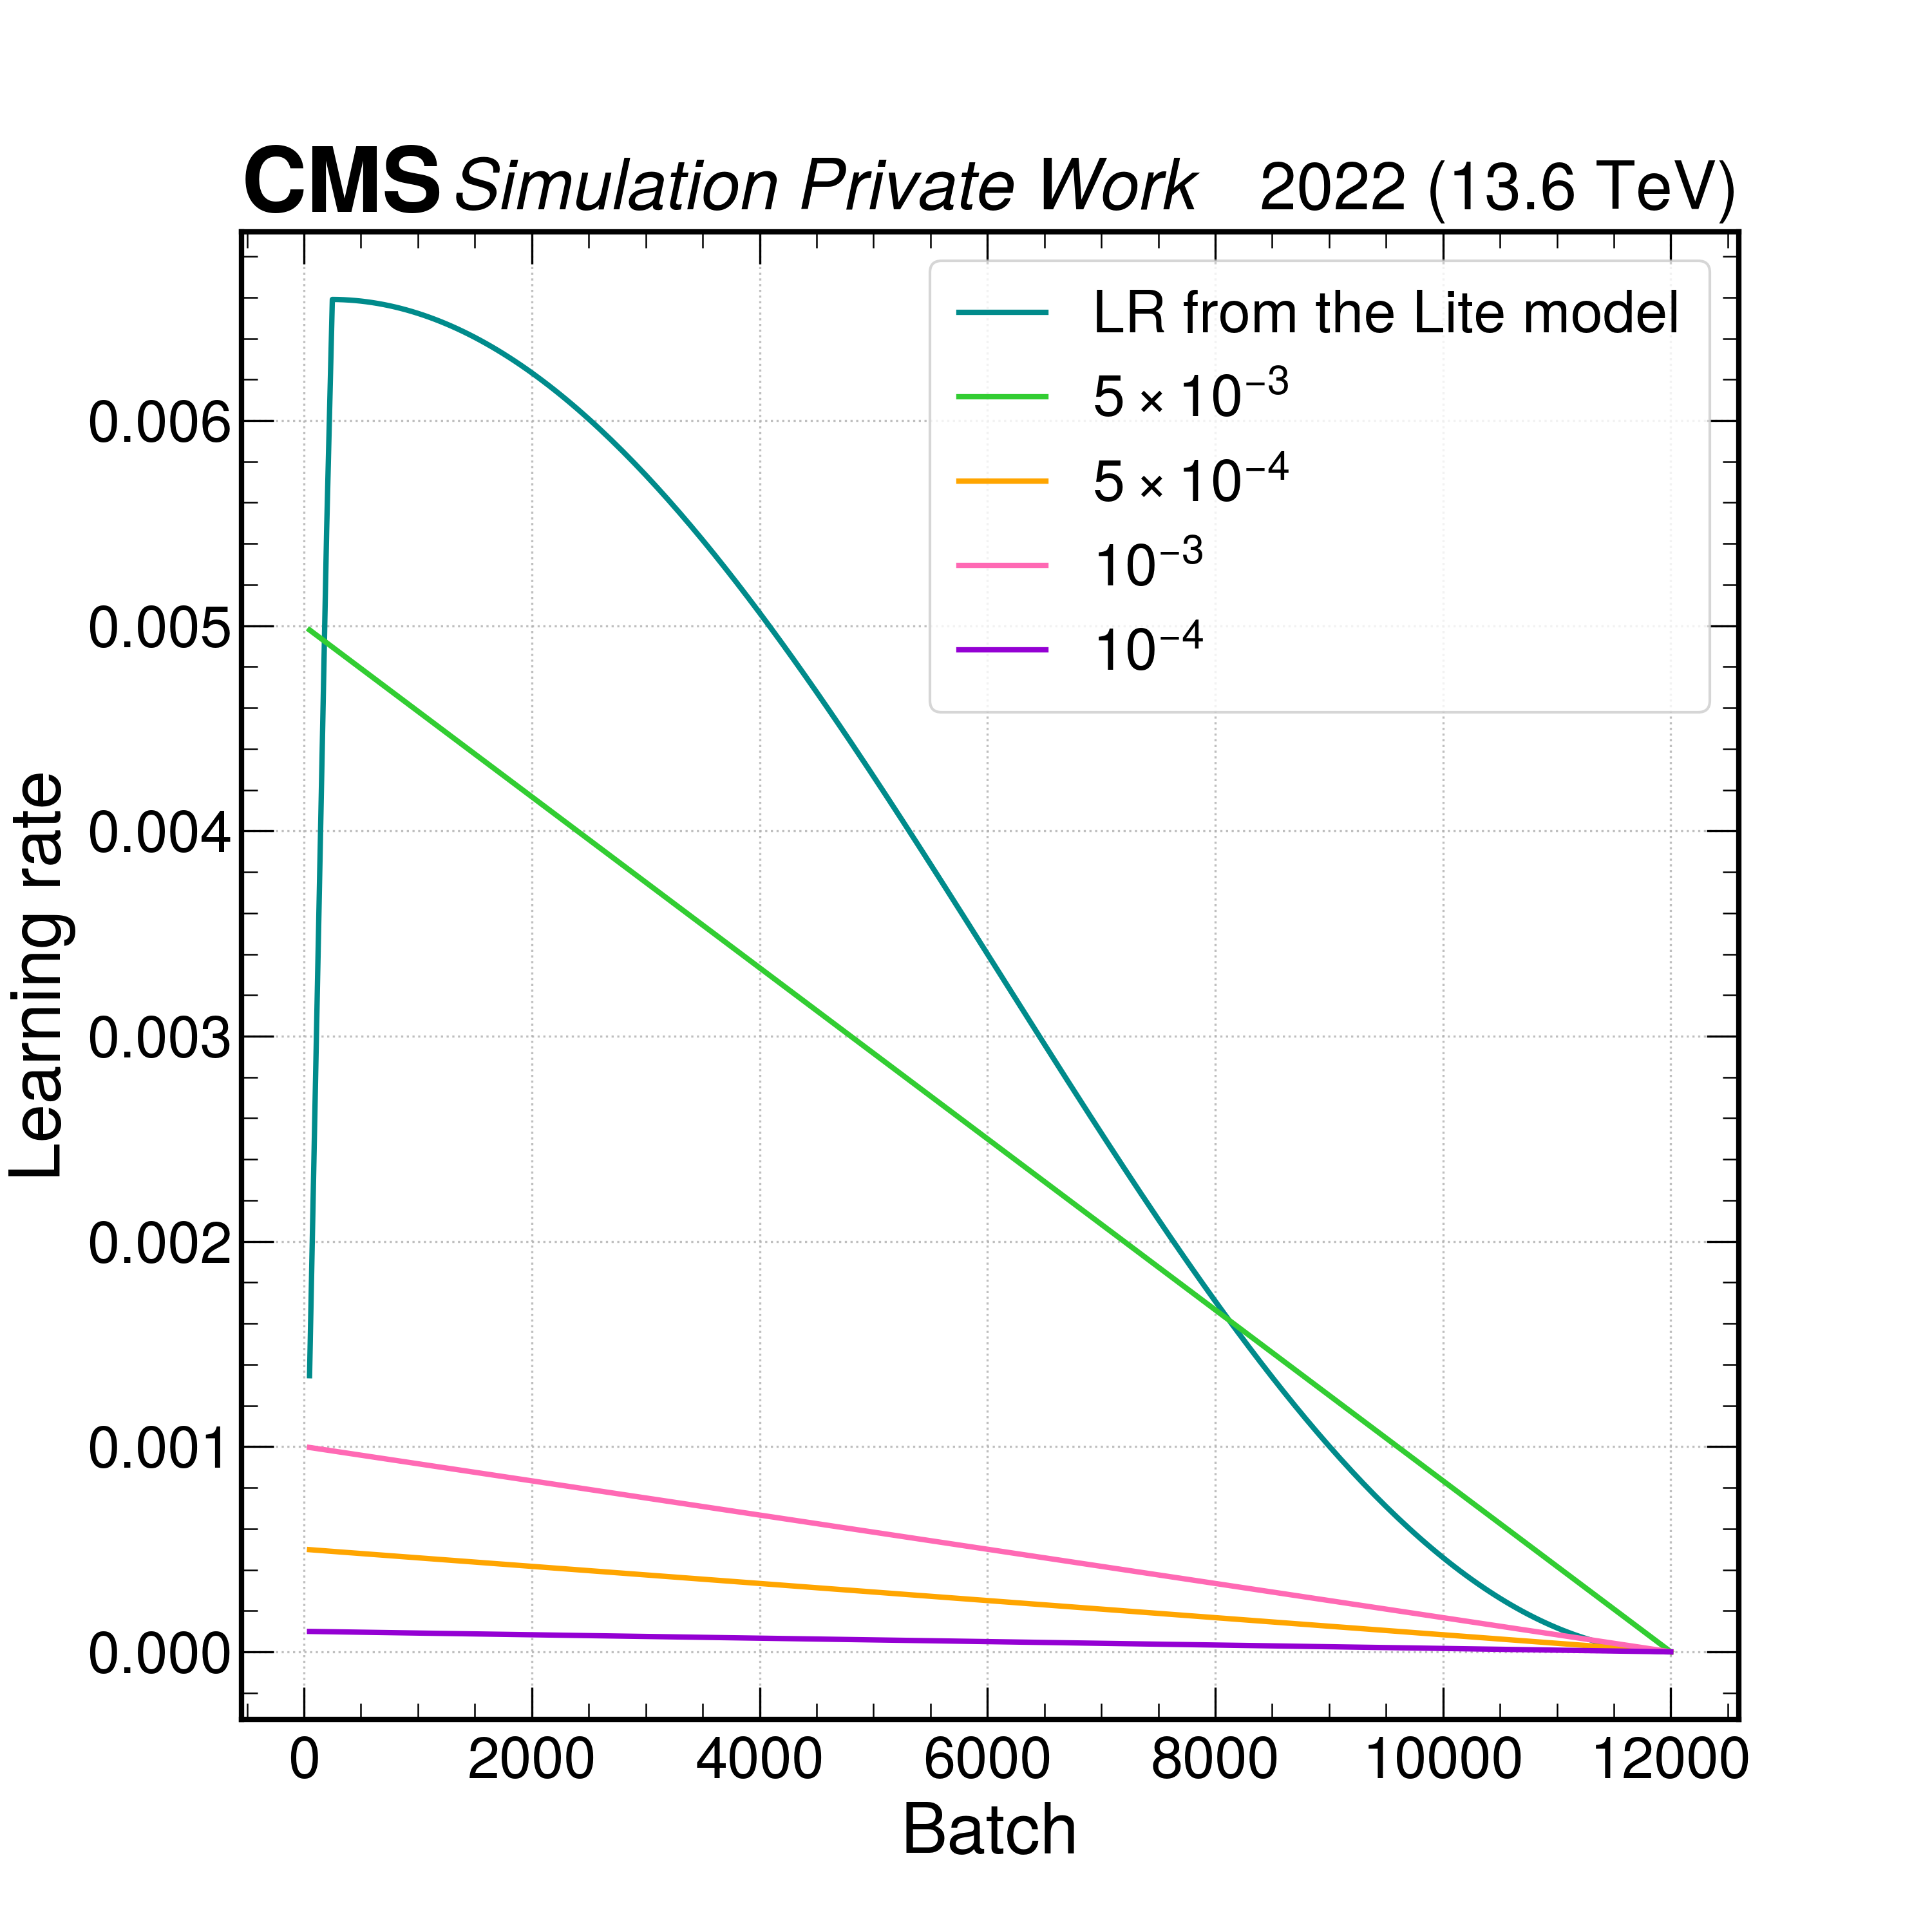
\includegraphics[width=0.6\linewidth]{Images/6.Improving/Variability Study/learning rate comp.png}
    \caption{Comparison of the learning rate (LR) used in the Lite model defined in Table \ref{table:comparison_models} (blue) to the learning rates presented in Table \ref{table: variation hyperpaparm }. We have also varied the LR warm-up cycles as well as the cycles as described in Table \ref{table: variation hyperpaparm } which explains the difference in the shape of the LR as a function of the batch size}
    \label{fig: lr comp}
\end{figure}

\begin{figure}[hbt]
    \centering
    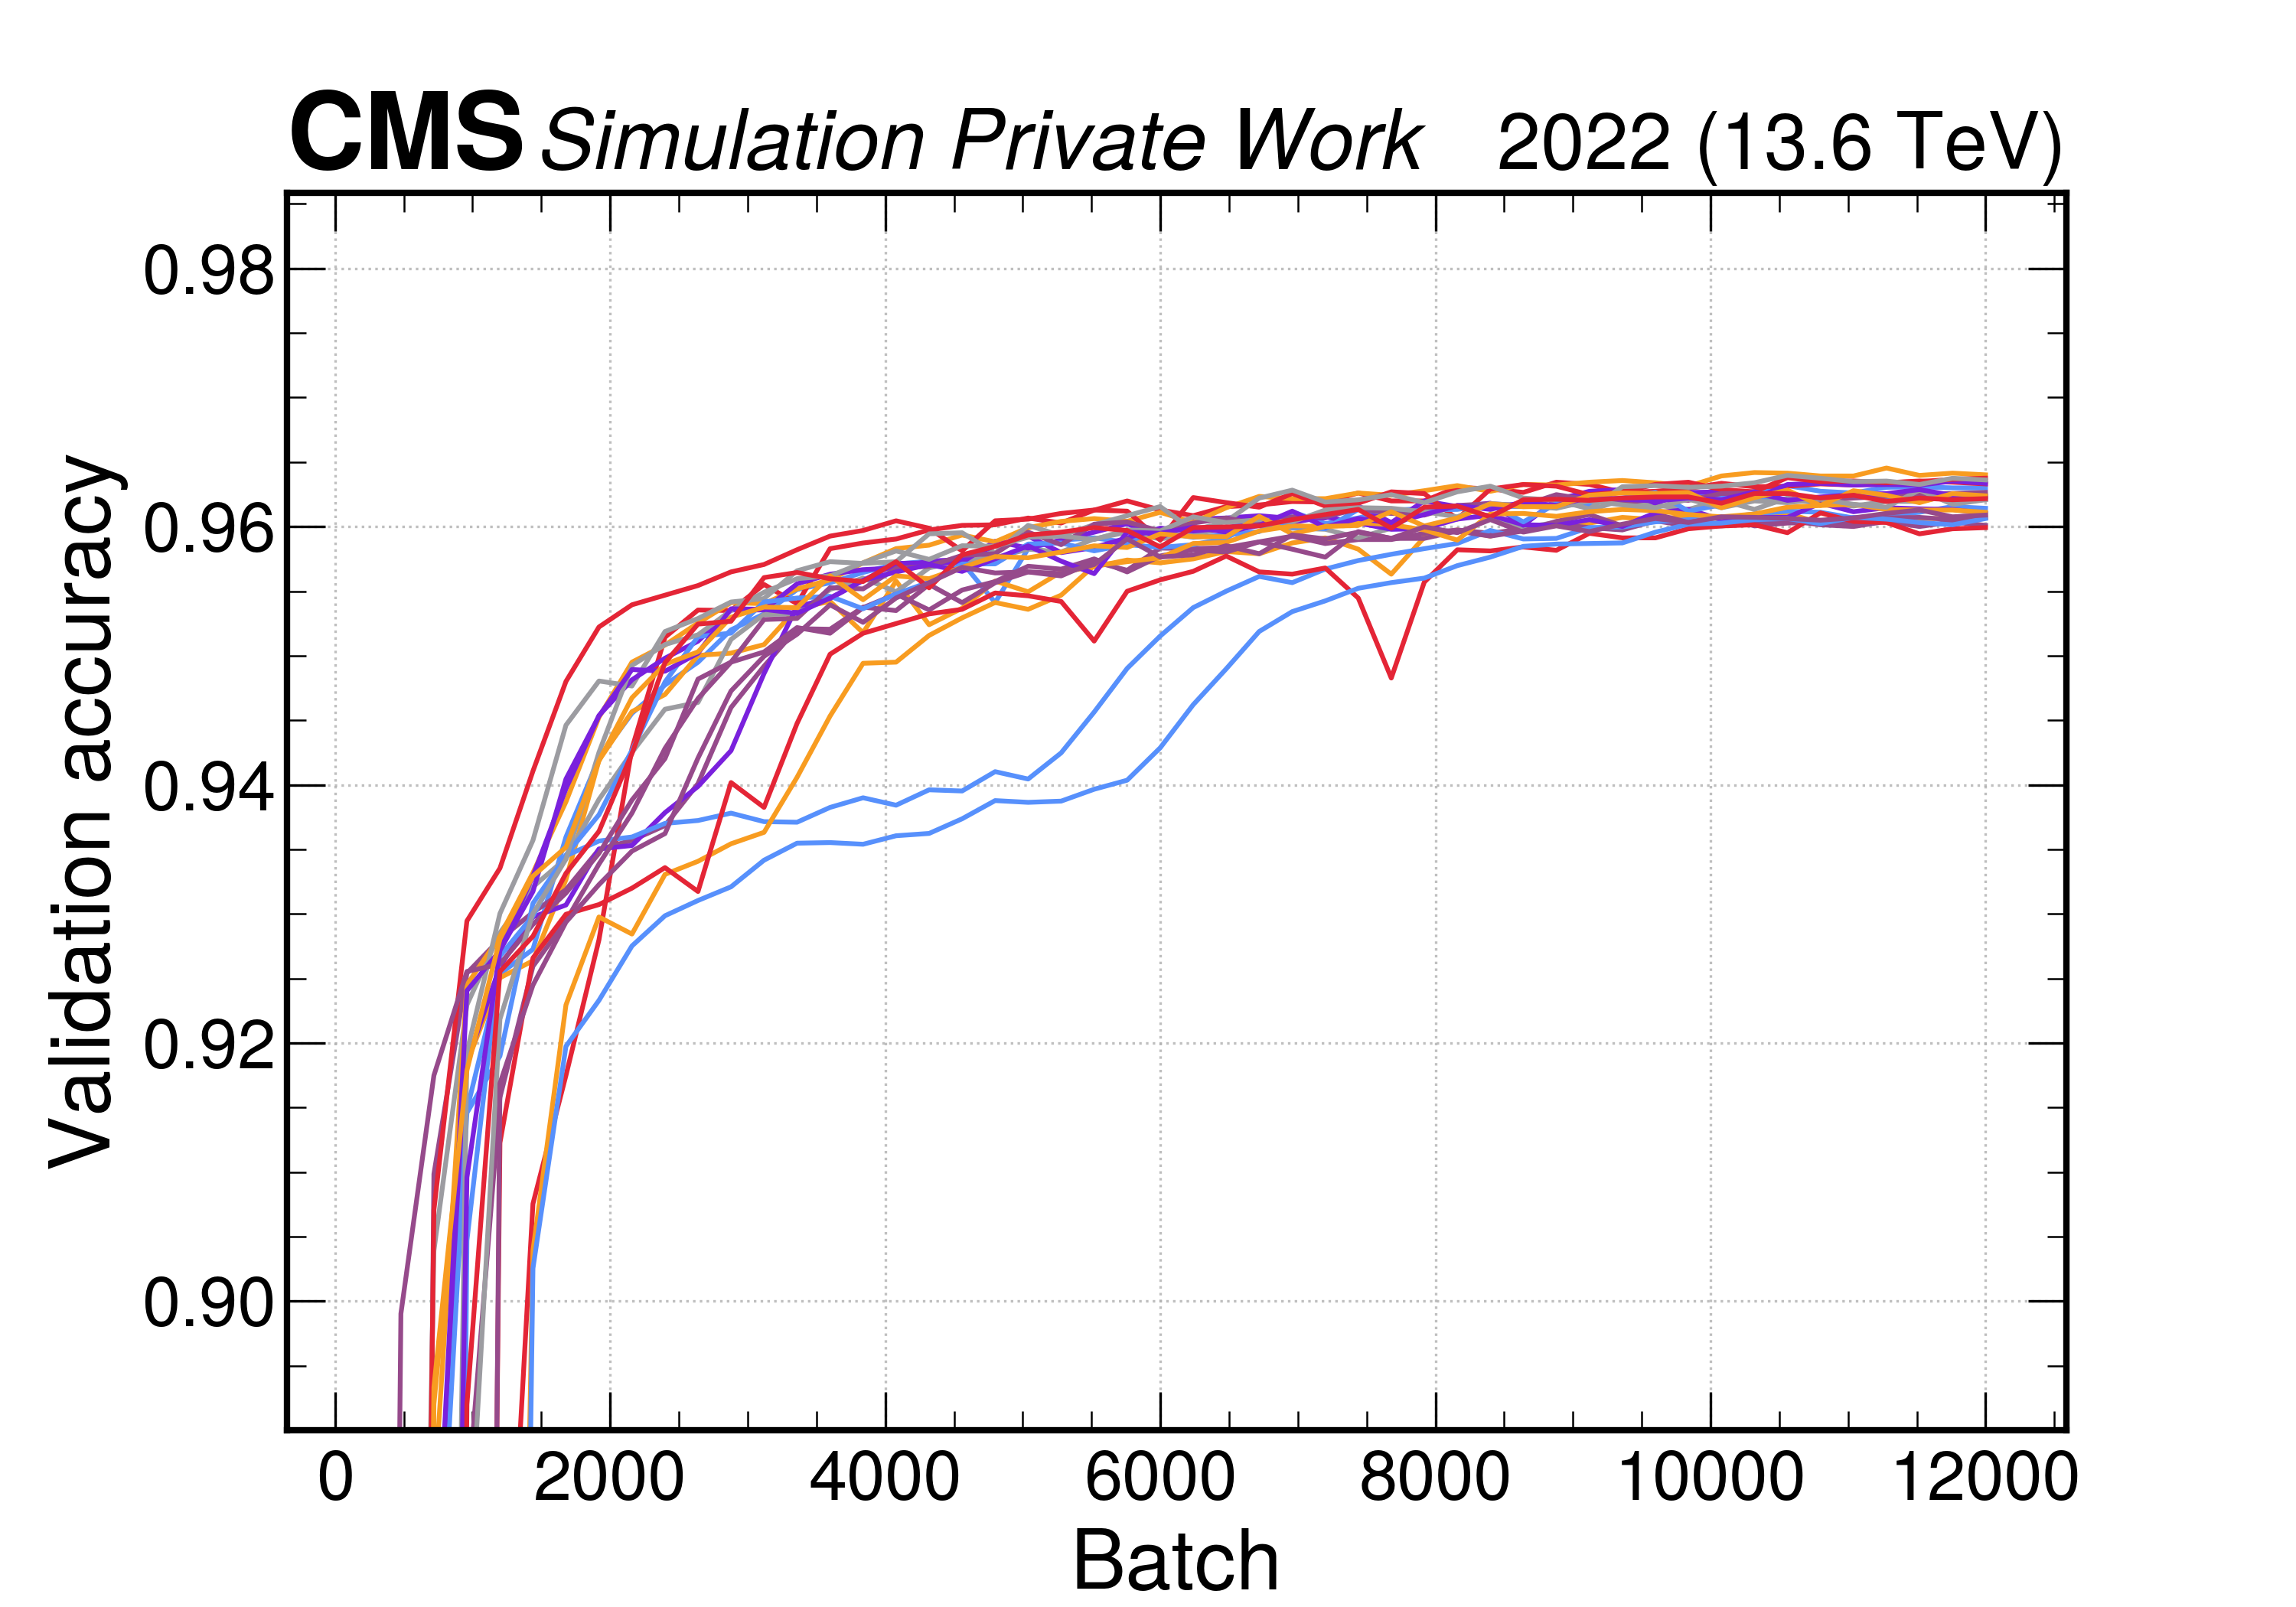
\includegraphics[width=0.7\linewidth]{Images/6.Improving/Variability Study/var 2048.png}
    \caption{Variability of the validation accuracy as a function of the batch size of the training with 5 jets as inputs pT reg, LR of $10^{-4}$, LR cycle and warm-up cycles equal to 0, a batch size of 2048 and 50 epochs}
    \label{fig: stable test}
\end{figure}

\begin{figure}[hbt]
    \centering
    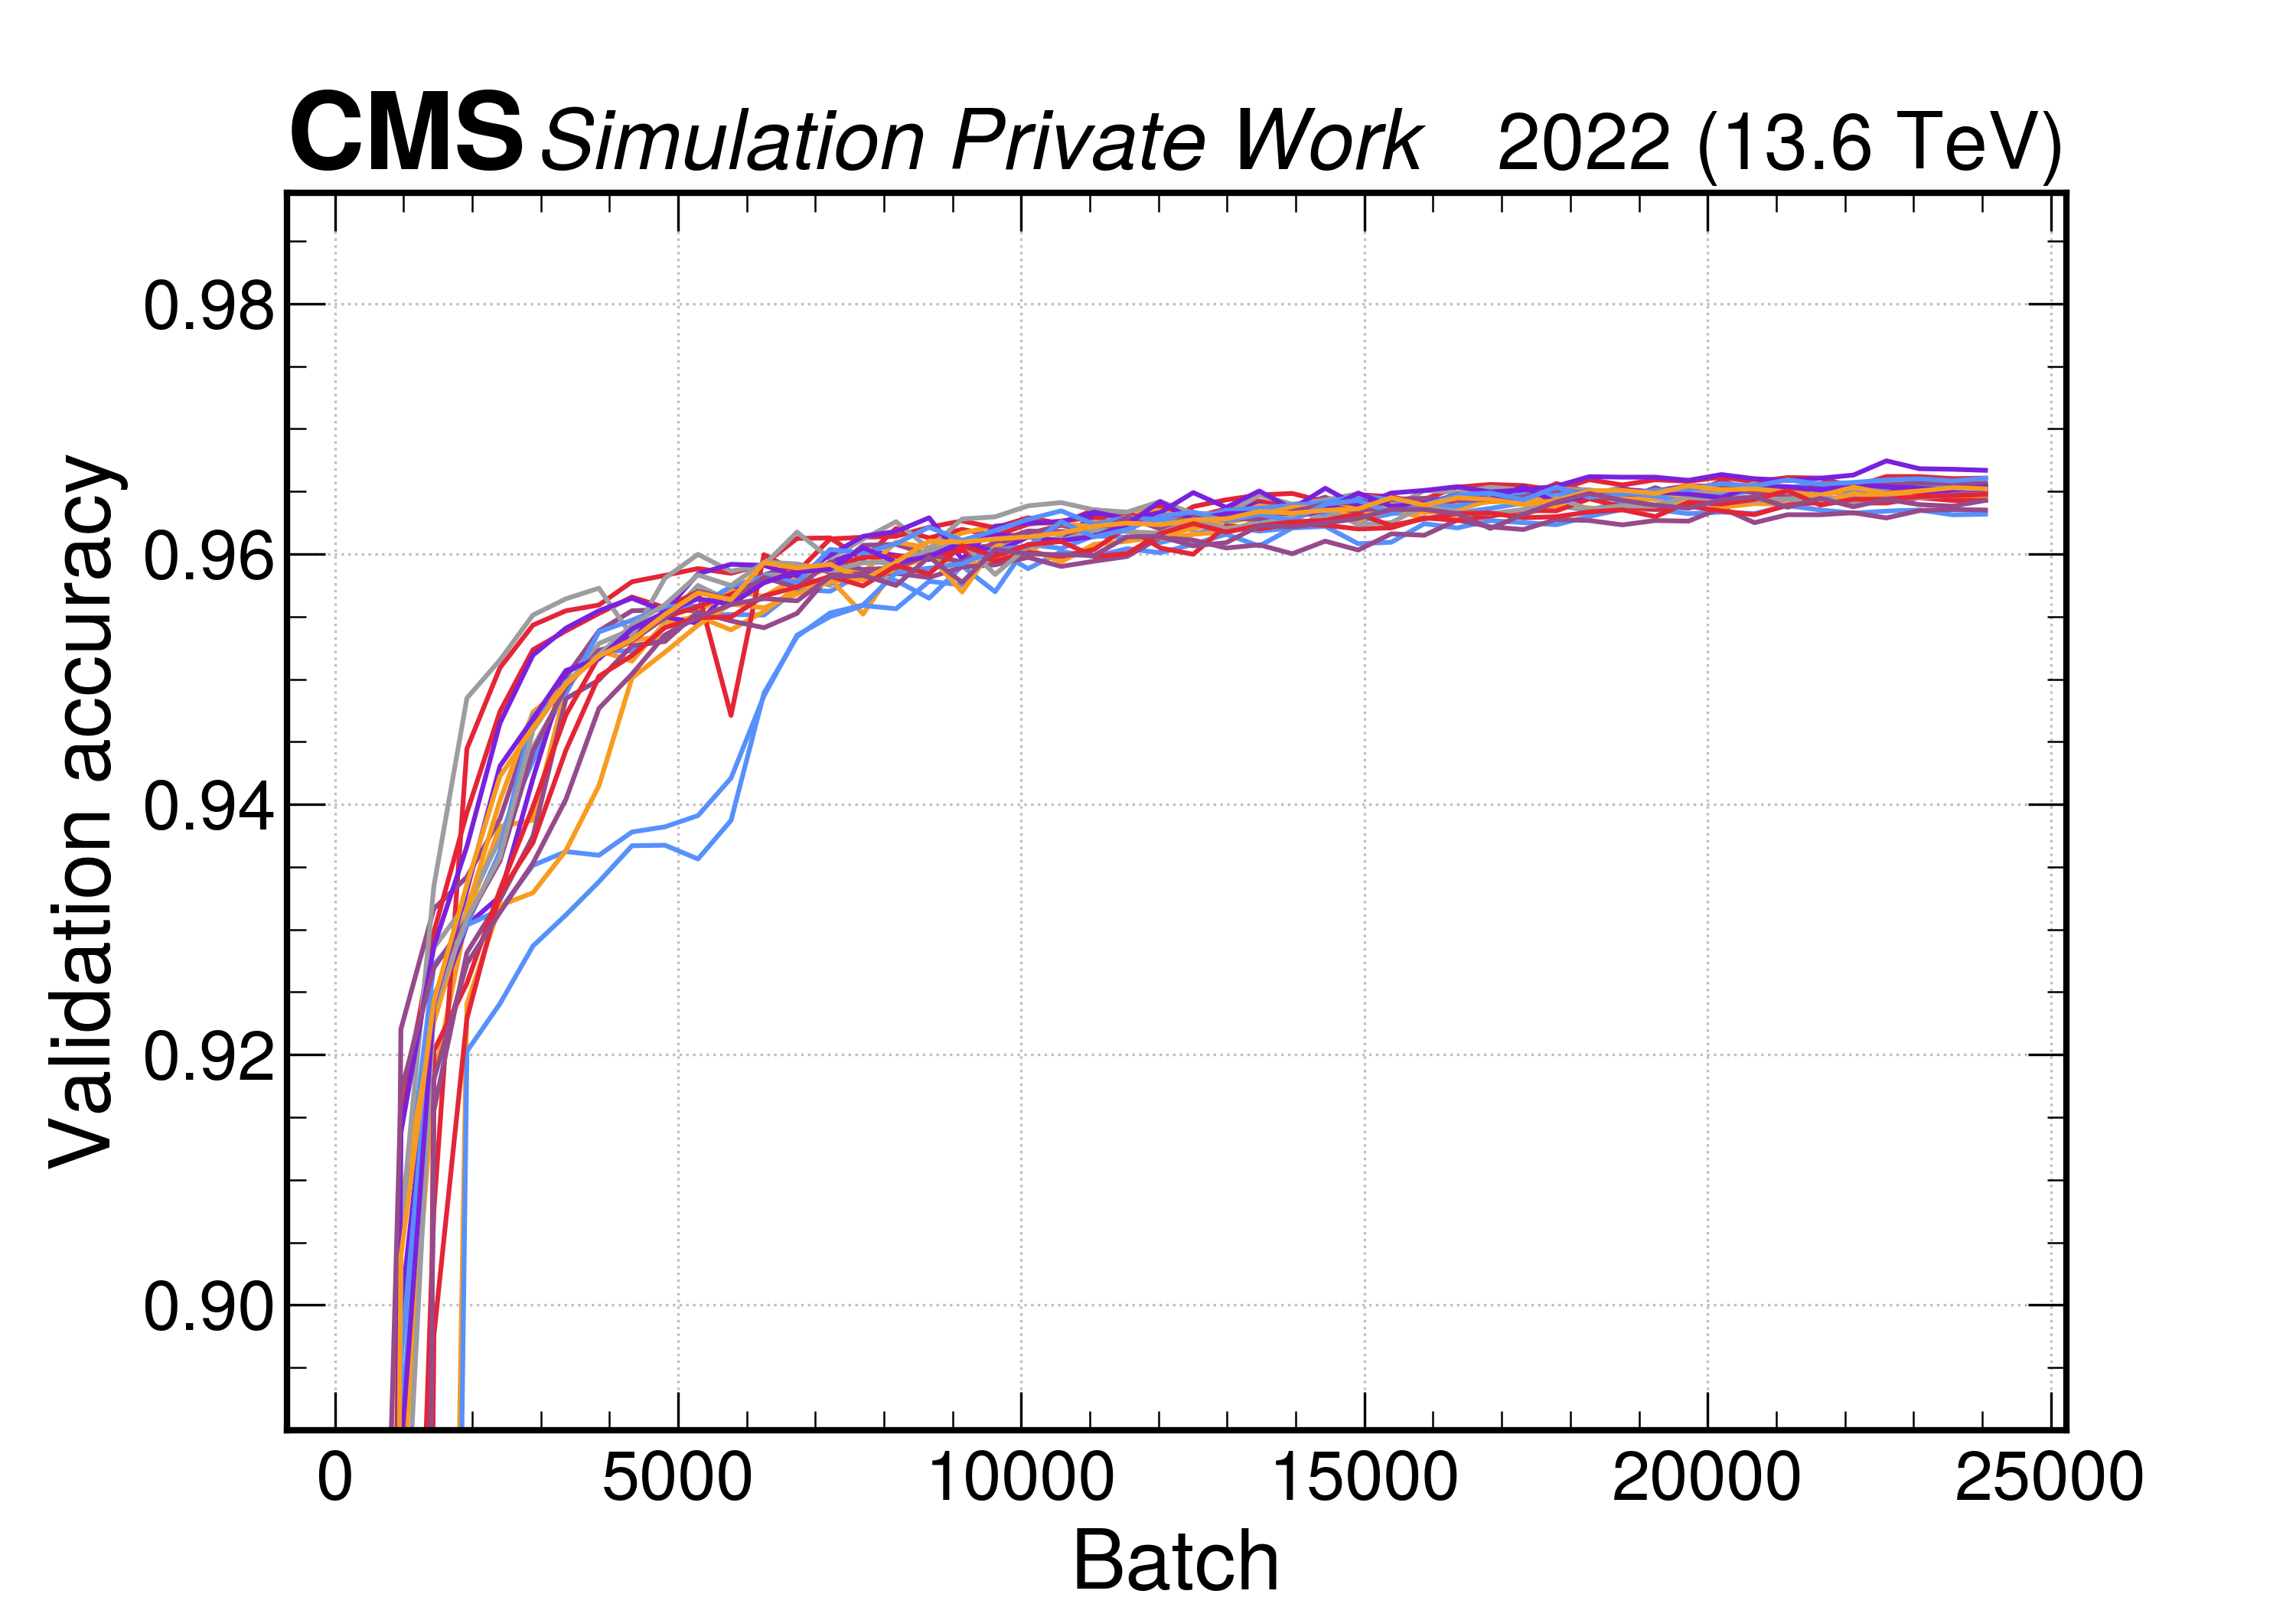
\includegraphics[width=0.7\linewidth]{Images/6.Improving/Variability Study/var 1024.png}
    \caption{Variability of the validation accuracy as a function of the batch size of the training with 5 jets as inputs pT reg, LR equal to $10^{-4}$, LR cycle and warm-up cycles equal to 0, a batch size of 1024 and 50 epochs}
    \label{fig: stable test 1024}
\end{figure}



Finally, we studied the difference in the efficiency when varying the number of epochs. In Figure \ref{fig: epoch diff} we observe that the validation accuracy is improved by around 0.4\% when using 300 epochs. When increasing the number of epochs to 300, the trainings are completed in four hours instead of half an hour. In conclusion, after this study the most stable and efficient configuration is given by the parameters showed in Table \ref{table: stable model} .

\begin{figure}[hbt]
    \centering
    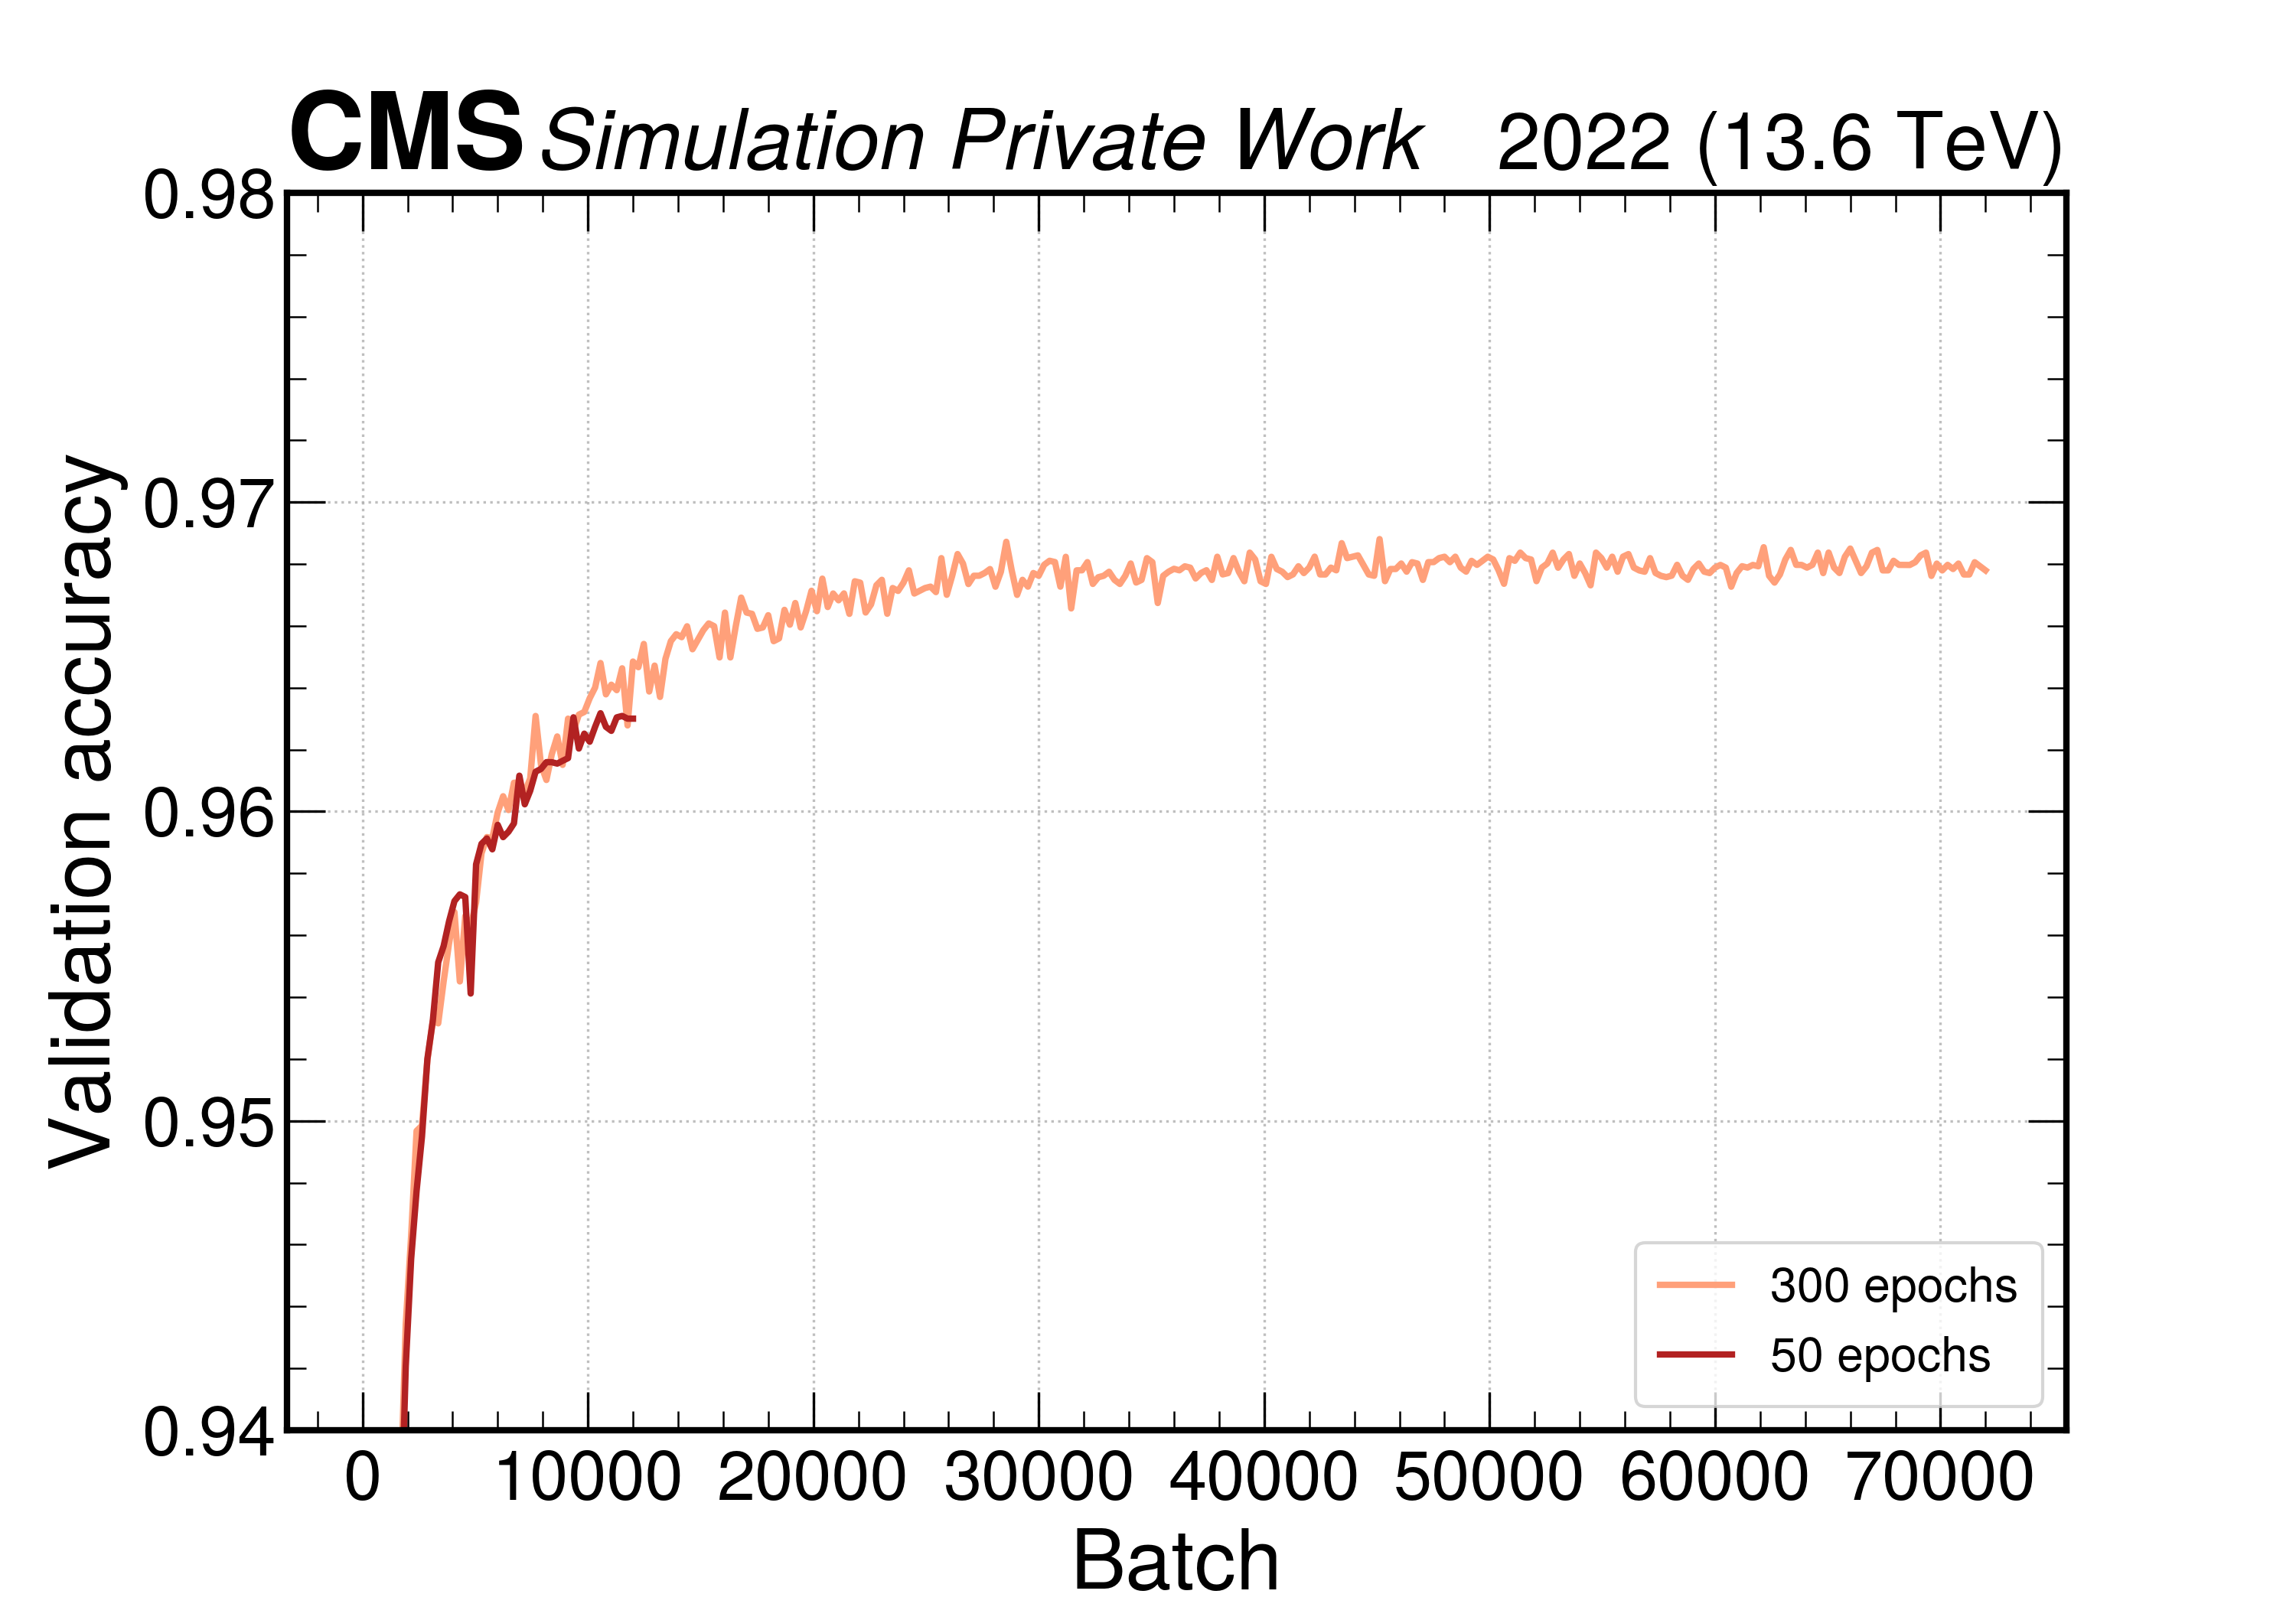
\includegraphics[width=0.7\linewidth]{Images/6.Improving/Variability Study/epoch comp.png}
    \caption{Comparison in the number of epochs of performance the training with 5 jets as inputs using our stable model}
    \label{fig: epoch diff}
\end{figure}

\begin{table}[hbt]
\centering
\begin{tabular}{|c|c|}
 \hline
 Parameters  & Stable model  \\
 \hline
 Learning rate &  $10^{-4}$ \\
 \hline
 Learning rate warmup cycles &  0\\
 \hline
  Learning rate cycles & 0\\
 \hline
 Batch size & 2048 \\
 \hline
 Number of epochs & 300 \\
 \hline
\end{tabular}
\caption{Configuration for the Stable model}
\label{table: stable model}
\end{table}


\newpage

\subsection{Grid search} \label{subsection: grid search}

In the following sections we will stick to the 5 jet \pt reg model using the Stable model hyper-parameters defined in Table \ref{table: stable model} instead of the Lite model ones defined in Table \ref{table:comparison_models}. As a last test to increase the performance of the 5 jets \pt reg Stable model, we perform a grid search, thanks to which we should find thee optimal configuration of hyper-parameters.

To do so, we used the features of the Stable model and changed the hyperparameters presented in Table \ref{table: parameters for the grid search}, as they are the default ones proposed by SPANet for thee tuning. 
However, contrary to what is specified in Table \ref{table: stable model} for this grid search we use 50 epochs, as the difference in performance compared to 300 epochs showed in Figure \ref{fig: epoch diff} is very small, and the trainings are completed faster.
As shown in Table \ref{table: parameters for the grid search}, we give different possible values for the hyperparameters and then we perform several trainings combining them differently.
For the first three, SPANet can choose between a value among the ones reported in Table \ref{table: parameters for the grid search}, whereas for the L2 Penalty the network can choose any value in the range [1e-5 : 1e-3] (in log scale).
The final outcome of this search is the combination of hyperparameters that provides the best performance.  The optimal hyper-parameters obtained by this grid search are reported in Table \ref{table: parameters for the grid search} as well.

\begin{table}[hbt]
   \centering
   \begin{tabular}{|c|c|c|}
   \hline
    Hyper-parameters  &  Tested values & Optimal choice \\
    \hline
    Hidden dimension  &  \{32, 64, 96\} & 96 \\
    \hline
   Number of encoder layers & \{5, 6, 7, 8\} & 5 \\
    \hline
    Number of branch embedding layers &  \{1, 2, 3, 4\} & 3 \\
    \hline
     Number of branch encoder layers & 4 & 4\\
    \hline
    Number of regression layers & 3 & 3 \\
    \hline
    Number of classification layers & 1 & 1\\
    \hline
    Focal gamma & 0.0 & 0.0 \\
    \hline
    L2 Penalty & [1e-5 : 1e-3] & $7.3\times 10^{-4}$ \\
    \hline
   \end{tabular}
   \caption{Hyper-parameters modified during the grid search to increase the performance of our network. The second column shows the possible values that can be chosen by SPANet during the search. The last column shows the final optimal hyper-parameters determined by the grid search}
   \label{table: parameters for the grid search}
\end{table}

\newpage
By using these new hyperparameters the optimal model used for the analysis has 5.1 M trainable parameters compared to 0.5 M in the Stable model. 
As shown in Figure \ref{fig: comp grid search}, by using this new hyperparameters, 
we do not increase significantly the performance compared to the Stable model performance. 
Hence, we decided to use the hyperparameters from the Stable Model.

\begin{figure}[hbt]
    \centering
    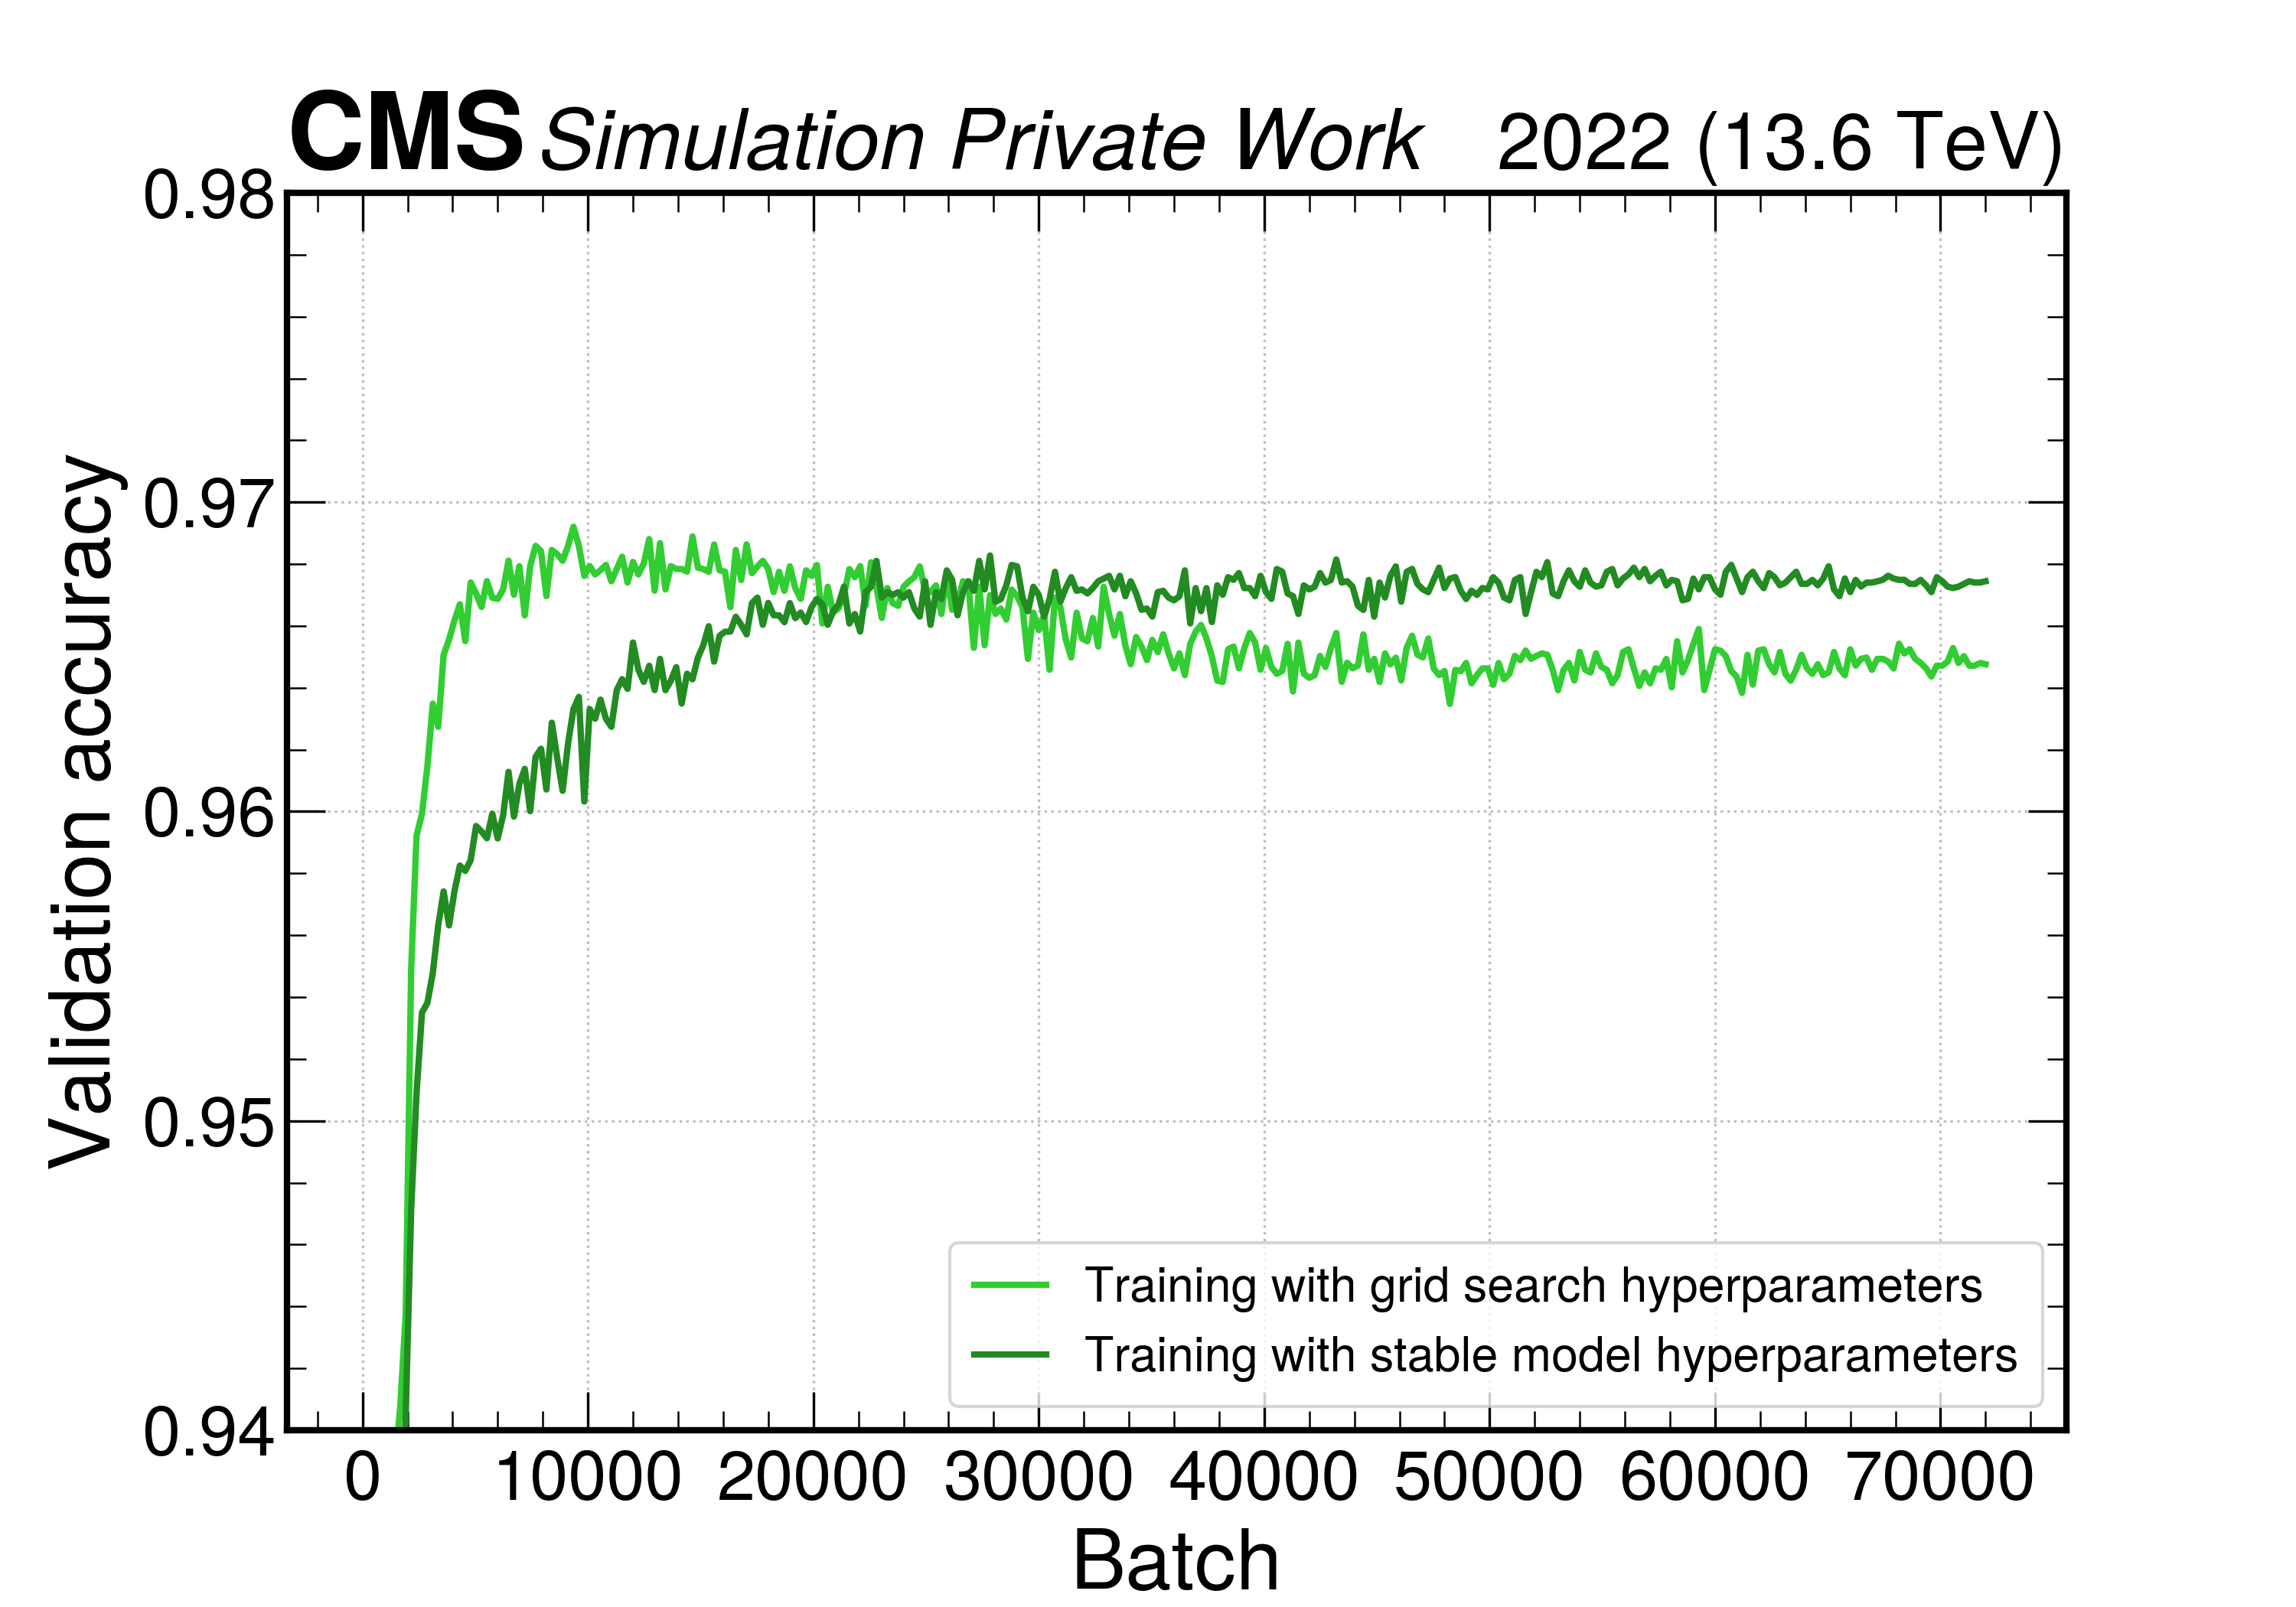
\includegraphics[width=0.6\linewidth]{Images/6.Improving/Grid search/grid search.png}
    \caption{Comparison of the training using the Stable model parameters and the hyperparameters given by the grid search}
    \label{fig: comp grid search}
\end{figure}

%Do i mention other traiinngs done by Mathieu?

\clearpage

\subsection{Introducing \kl in the trainings} \label{subsection: kl}

As explained in section \ref{section: HH4b}, by measuring the di-Higgs production we are aiming to study 
the Higgs boson self coupling parameter $\lambda$. However, when \kl (defined in section \ref{section: HH4b}) varies, the kinematics 
of our process change and therefore the distributions of some of our observable. To give an example of the difference in the kinematics, we show in Figure \ref{fig: mhh dist} the $m_{HH}$ distribution for different \kl. Therefore, we would like to add this feature to the SPANet trainings. 
In order to do so, we employ several signal samples with different values of $\kappa_\lambda 
\in \{-2.0, -1.0, 0.0, 0.5, 1.0, 1.5, 2.0, 2.45, 3.0, 3.5, 4.0, 5.0\}$. 

%(Do I specify that we performed a validation study between the private and public samples?)

\begin{figure}[hbt]
    \centering
    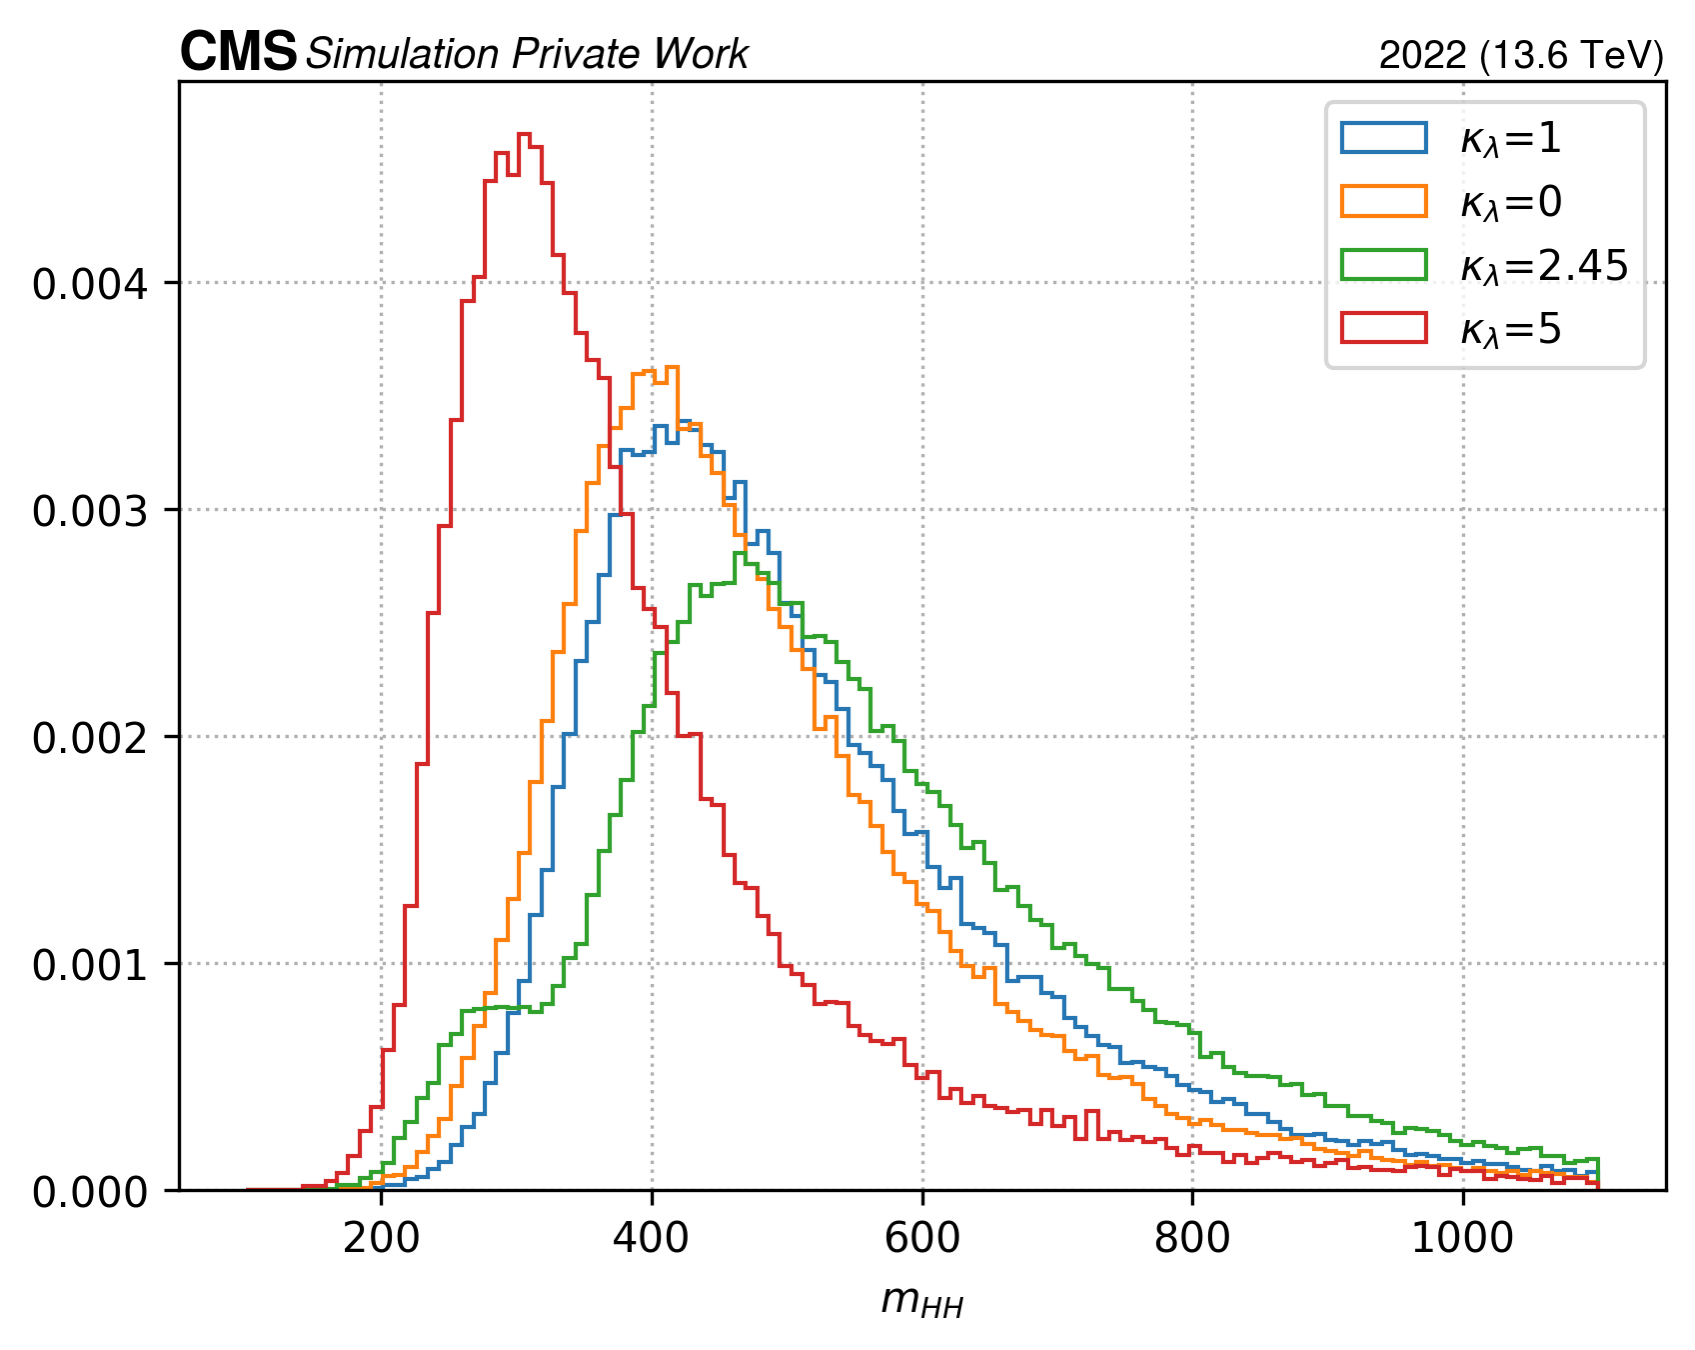
\includegraphics[width=0.5\linewidth]{Images/6.Improving/kappa lambda/mhh distribution for diff kl.png}
    \caption{$m_{HH}$ distribution for different values of \kl}
    \label{fig: mhh dist}
\end{figure}


\vspace{0.2cm}

In this section we compare the difference of performance when training SPANet with \kl samples instead of SM samples. In addition we also compare the difference in performance when adding the explicit value of \kl per event as global input, meaning adding the value of \kl per event as global input. In order to do so, we compare the trainings presented in Table \ref{table:kl as input or not}. The naming "Tight cuts" refers to the Tight cuts presented in section \ref{subsection:cutflows}, that we have been using in the previous sections. 

\begin{table}[h!]
\centering
    \begin{tabular}{|M{4cm}|M{7cm}|}
     \hline
     Training  & Configuration \\
     
     \hline
     
    SPANet - \kl - Tight selection &  5 jets as inputs:\footnotesize 
    \begin{itemize}[itemsep=0.001em]
        \item \pt
        \item $\eta$
        \item $\phi$
        \item b-tag
        \item Train file containing events with different \kl
        \item \kl not an explicit input to the network
    \end{itemize} \\
     
     \hline
     
    SPANet - \kl (\kl inputs)- Tight selection &  5 jets as inputs: \footnotesize 
    \begin{itemize}[itemsep=0.001em]
        \item \pt
        \item $\eta$
        \item $\phi$
        \item b-tag
        \item Train file containing events with different \kl
        \item \kl as global input
    \end{itemize} \\
     
     \hline
     
      SPANet - SM - Tight selection &  5 jets as inputs: \footnotesize 
    \begin{itemize}[itemsep=0.001em]
        \item \pt
        \item $\eta$
        \item $\phi$
        \item b-tag
        \item Train file containing only events with SM coupling 
    \end{itemize}\\    
     \hline
    \end{tabular}
    \caption{Training configurations used to test the difference when using SM samples or \kl samples. We also test the difference when adding \kl as an explicit input to the network}
    \label{table:kl as input or not}
\end{table}


%Figures \ref{fig: kl kl input or no input} and \ref{fig: mhh kl input or no input} show the total pairing efficiency as a function of \kl and $m_{HH}$ respectively of the models presented in Table \ref{table:kl as input or not}.

Figure \ref{fig: kl kl input or no input} shows the total pairing efficiency as a function of \kl. We find that by training our model using a sample with different \kl, the pairing performance is improved with respect to the SPANet-SM training. However, we observe that using \kl as an explicit input to our network does not improve our performance. The same conclusion can be drawn from Figure \ref{fig: mhh kl input or no input}, where we show the total pairing efficiency as a function of $m_{HH}$. This is expected since \kl and $m_{HH}$ are correlated. Especially, in the low $m_{HH}$ mass region, we can see a large improvement compared to the trainings using only SM samples. This improvement in the pairing efficiency with respect to the training using SM samples is expected as well since by adding events with different \kl as can be seen in Figure \ref{fig: mhh dist} we are adding a lot of new events in the low $m_{HH}$ spectrum for the training. Finally, in both Figures \ref{fig: kl kl input or no input} and \ref{fig: mhh kl input or no input}, it is observed that the SPANet pairing efficiency outperforms the Run 2 approach on the $D_{HH}$-method one finds that the pairing efficiency using the $D_{HH}$-method is outperformed.

\begin{figure}[hbt]
    \centering
    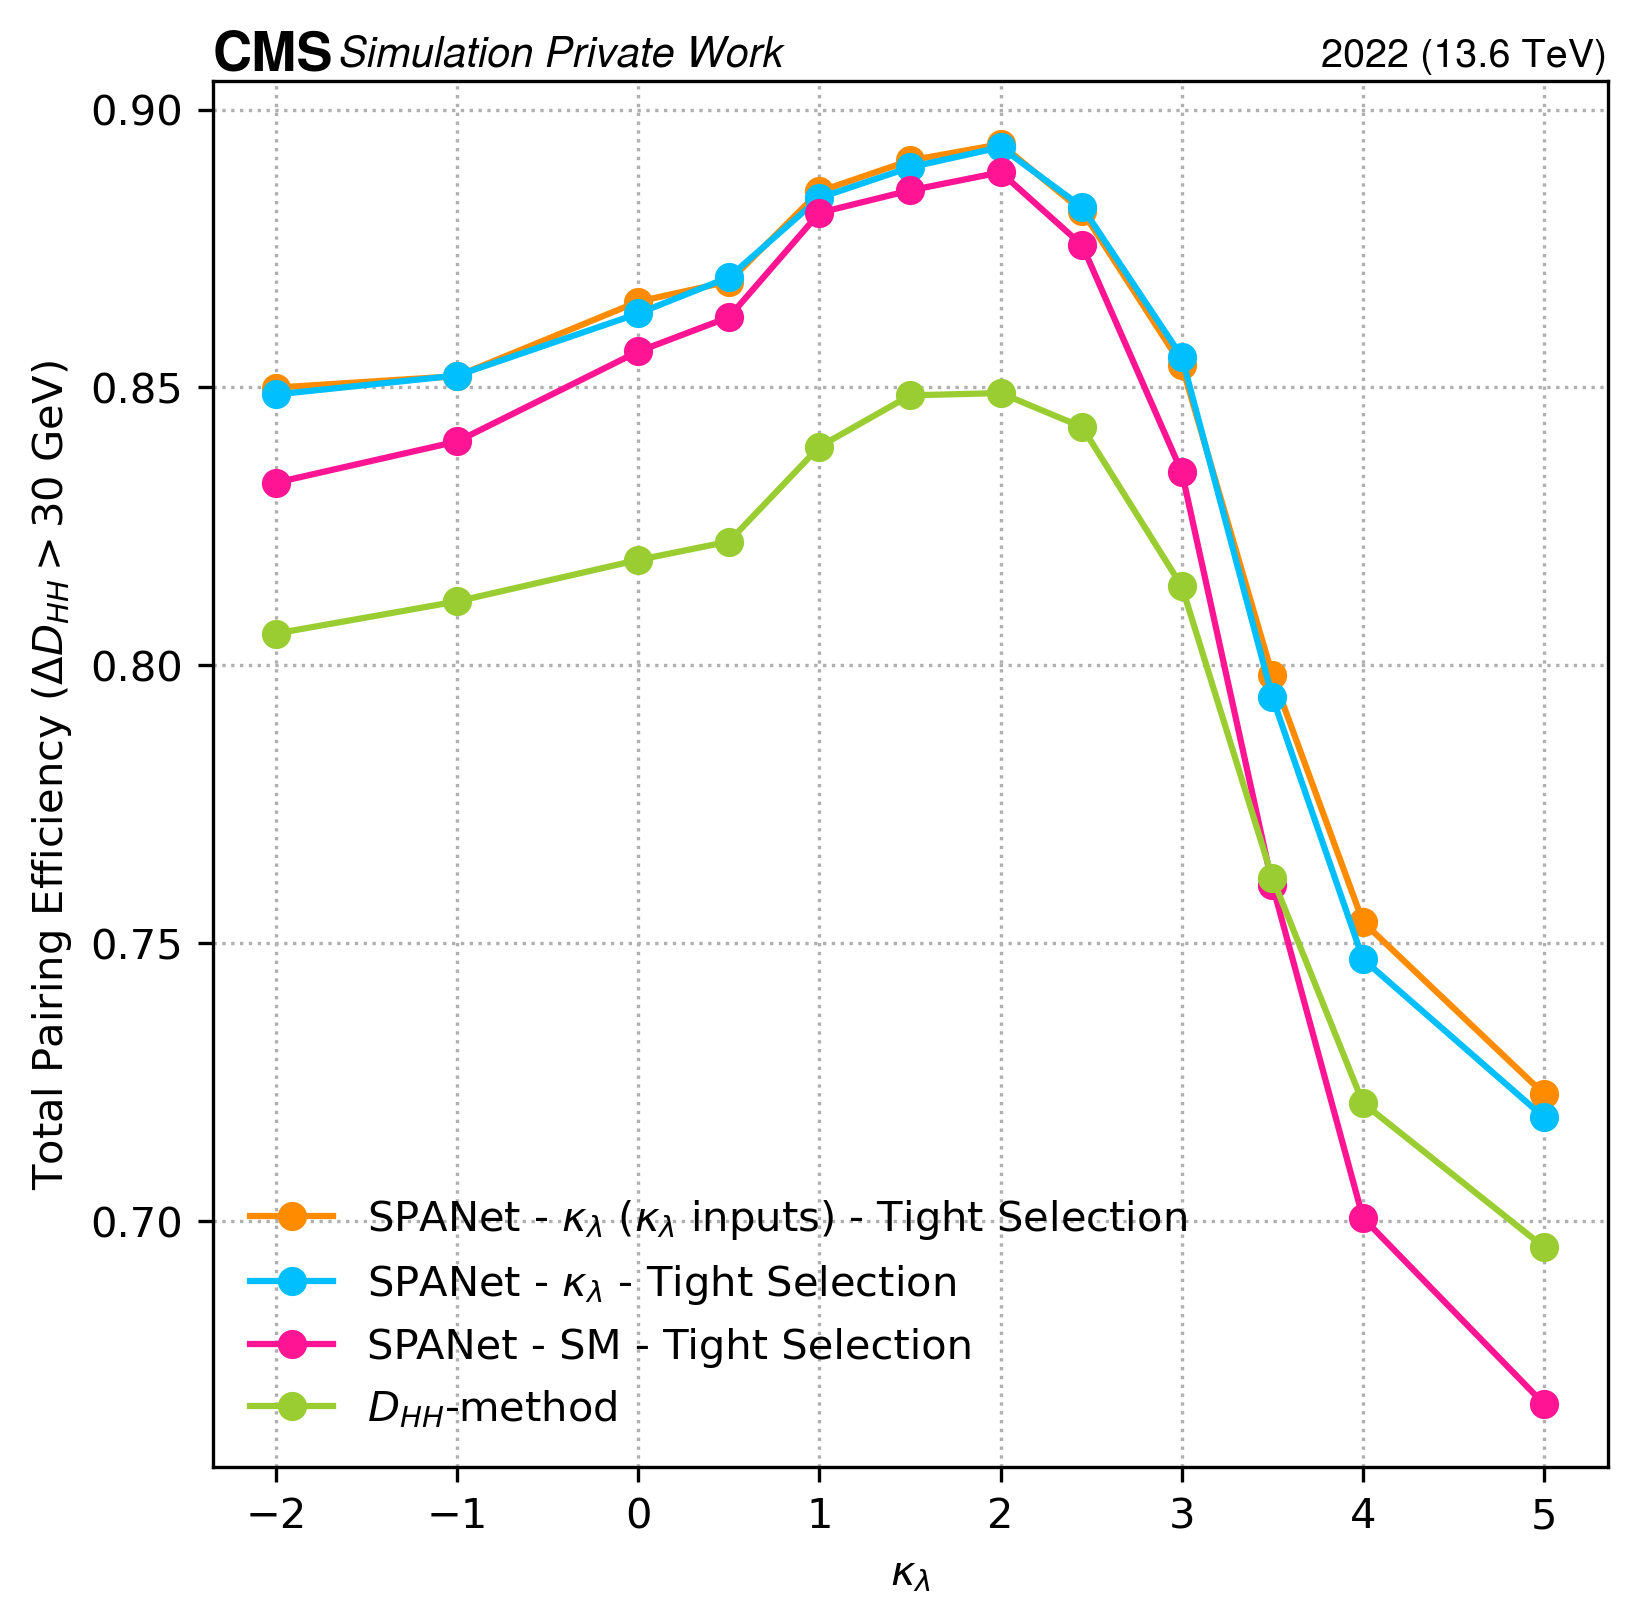
\includegraphics[width=0.6\linewidth]{Images/6.Improving/kappa lambda/kl inout vs no input.png}
    \caption{Total pairing efficiency as a function of \kl for the different training configuration presented in Table \ref{table:kl as input or not}}
    \label{fig: kl kl input or no input}
\end{figure}

\begin{figure}[hbt]
    \centering
    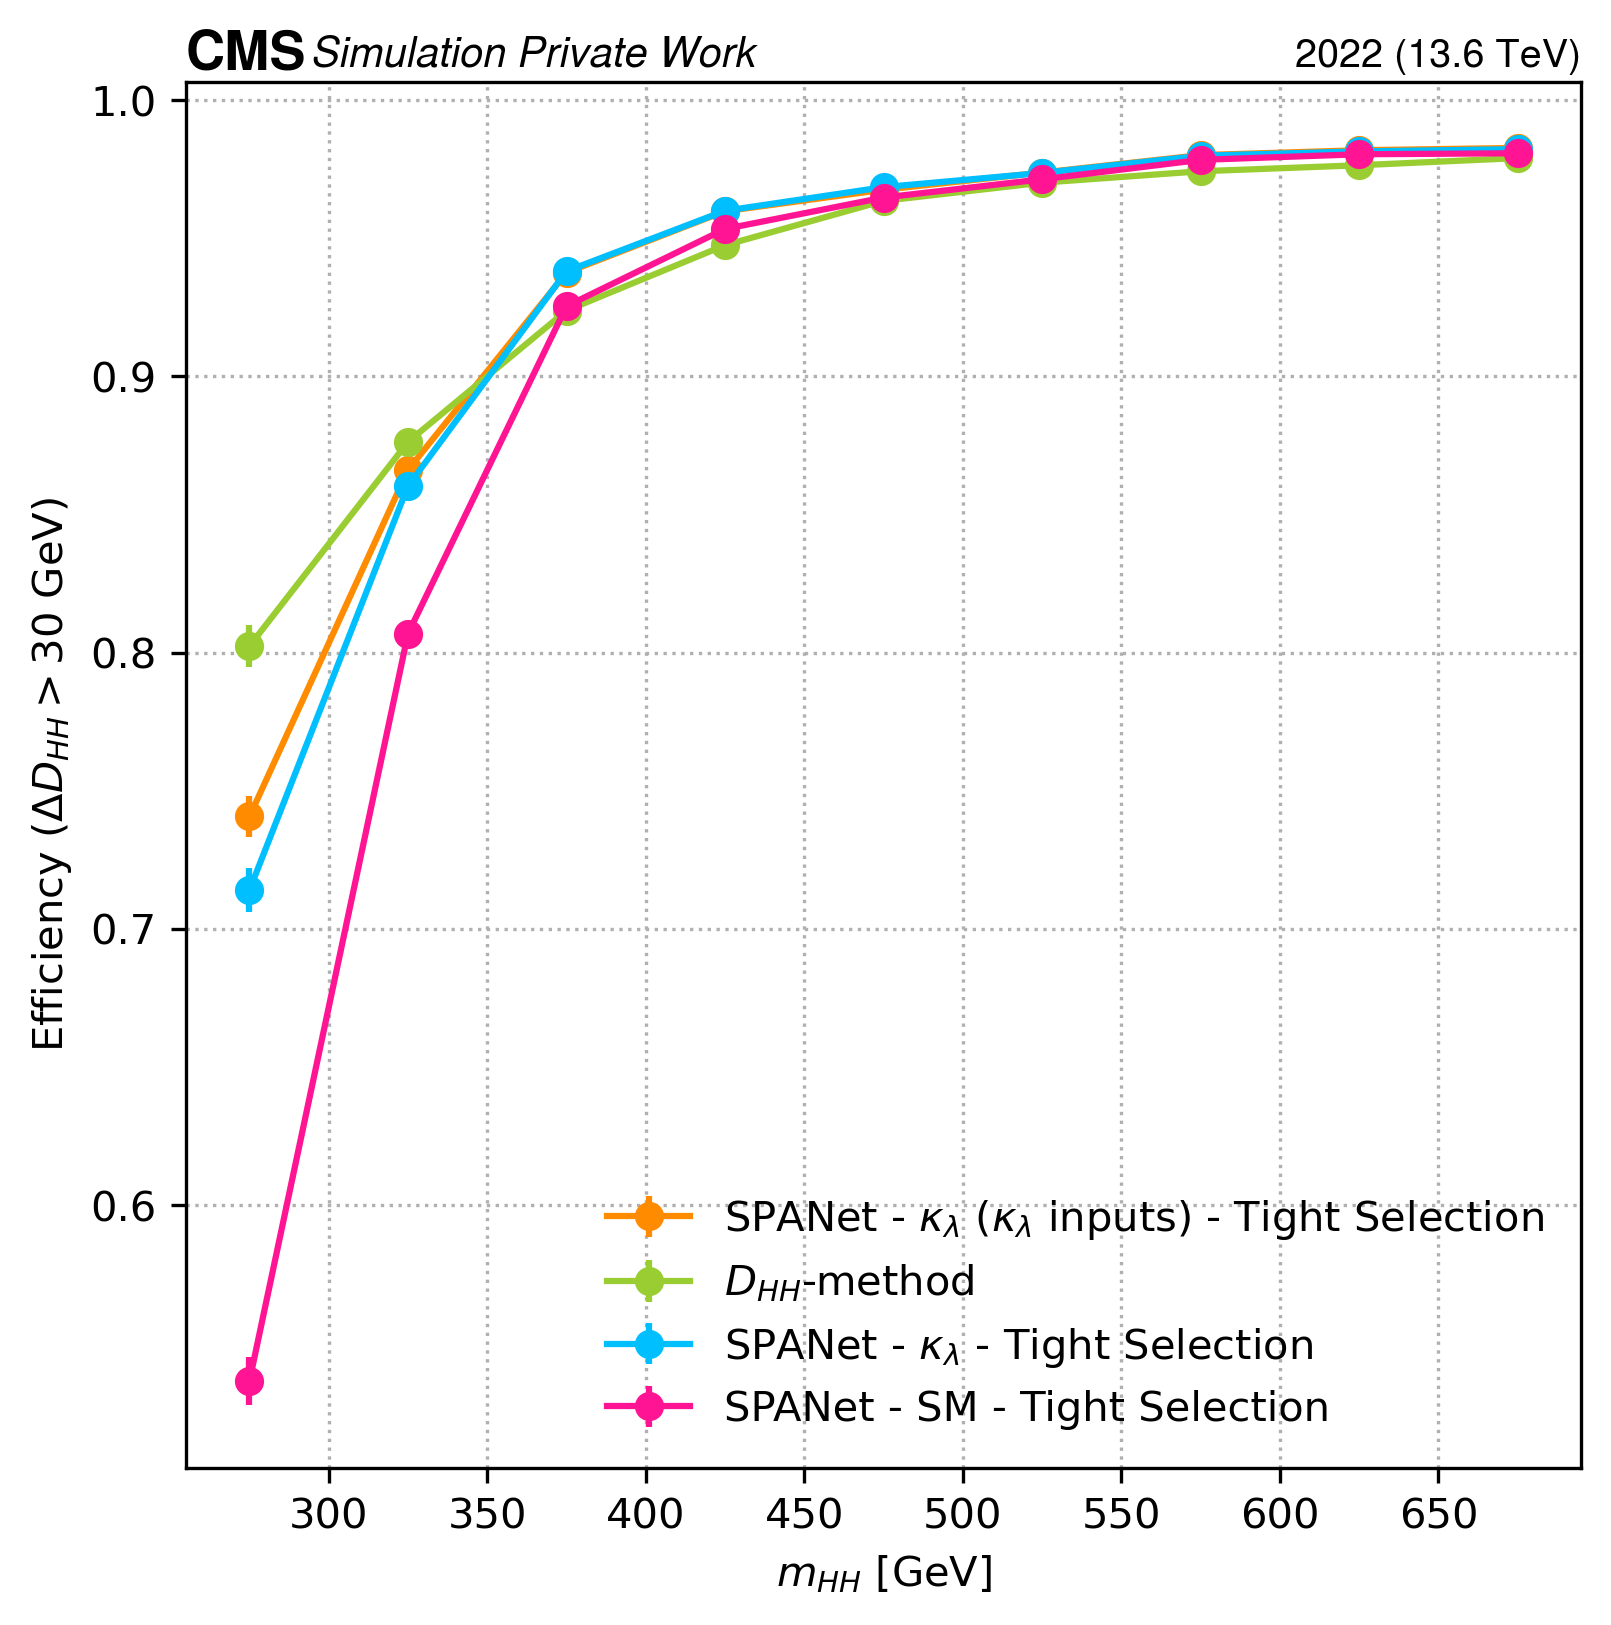
\includegraphics[width=0.6\linewidth]{Images/6.Improving/kappa lambda/eff diff kl vs kl input.png}
    \caption{Total pairing efficiency as a function in $m_{HH}$ for the different training configuration presented in Table \ref{table:kl as input or not}}
    \label{fig: mhh kl input or no input}
\end{figure}

Since we concluded from these figures that adding \kl as an explicit input does not improve our efficiency, we will use the model where we do not explicitly add \kl as input since when we are evaluating our model on data, we can't know to which \kl corresponds each event. Therefore, since if we evaluate our model on either data or QCD it would be ambiguous what to give to \kl as input, we decide to stick to the SPANet - \kl - Tight selection model.

In Table \ref{table: improvement} we show the values of the pairing efficiency as well as the total pairing efficiency for \kl $\in \{ 0 , 1 , 5 \} $ with our best model. From these values we see that by using the training SPANet - \kl - Tight selection, we have {4-8\%} absolute improvement with respect to the $D_{HH}$-method, as well as a {5-14\%} relative improvement. 

\begin{table}[h!]
\centering
\begin{tabular}{|M{2.5cm}||M{1.75cm}|M{1.75cm}||M{1.75cm}|M{1.75cm}||M{1.75cm}|M{1.75cm}|}
 \hline
 Training  & Pairing efficiency (\kl=1) &  Total pairing efficiency (\kl=1) & Pairing efficiency (\kl=0) &  Total pairing efficiency (\kl=0) & Pairing efficiency (\kl=5) &  Total pairing efficiency (\kl=5) \\
 \hline
  $D_{HH}$-method &  0.944 &  0.836 & 0.921 & 0.808 & 0.739 & 0.603\\
 \hline
 SPANet - \kl - Tight selection & 0.952  &  0.880 & 0.932 & 0.853 & 0.792 & 0.685 \\
 \hline
\end{tabular}
\caption{Comparison of the pairing efficiency and the total pairing efficiency between the $D_{HH}$-method and the training SPANet - \kl - Tight selection}
\label{table: improvement}
\end{table}

\subsection{Impact of different selection for the searches}

In the previous sections, Tight cuts (defined in Section \ref{subsection:cutflows}) were applied to the samples used for training and evaluation. Nevertheless, to have a better comparison to the AN (cite), the SPANet training should be evaluated on a sample where Loose cuts (defined in Section \ref{subsection:cutflows}) have been applied. Therefore, we verify if evaluating and training on samples with Loose cuts improves the SPANet pairing performance with respect to training on samples with Tight cuts but evaluating on a sample with Loose cuts. The configuration of training used for the comparison is reported on Table \ref{table:kl loose vs tight}

\begin{table}[h!]
\centering
\begin{tabular}{|M{2.5cm}|M{6cm}|}
 \hline
 Training  & Configuration  \\
 \hline
  SPANet - \kl - Tight selection &  5 jets as inputs:\footnotesize \begin{itemize}[itemsep=0.001em]
    \item \pt
    \item $\eta$
    \item $\phi$
    \item b-tag
    \item Tight cuts
    \item Train file containing events with different \kl but these are not given as explicit inputs to the network
 \end{itemize}  \\
 \hline
 SPANet - \kl - Loose selection &  5 jets as inputs: \footnotesize \begin{itemize}[itemsep=0.001em]
    \item \pt
    \item $\eta$
    \item $\phi$
    \item b-tag
    \item Loose cuts
    \item Train file containing events with different \kl but these are not given as explicit inputs to the network
 \end{itemize}  \\
 \hline
\end{tabular}
\caption{Configuration of trainings using a sample containing events with different \kl}
\label{table:kl loose vs tight}
\end{table}

In Figure \ref{fig: loose vd tight}, we show the total pairing efficiency as a function of \kl for the trainings presented in Table \ref{table:kl loose vs tight} both evaluated on the test file in which the Loose cuts where applied. We also compare them to the $D_{HH}$-method used in Run 2. From this figure, we can see that the performance is the same for the two trainings within the variability and that they both outperform the $D_{HH}$-method. Nevertheless, the test of the background mass sculpting shows (Figures \ref{fig: leading H mass dist} and \ref{fig: subleading H mass dist}) that there is a significant difference between training on Loose or Tight cuts. We conclude that training on Loose cuts sculpts significantly more the mass both the leading and the subleading Higgs. Since this is a feature that we want to avoid for our model, we will stick to the training using Tight cuts but in the next results that will be presented we will always evaluate our model in Loose cuts.

\begin{figure}[hbt]
    \centering
    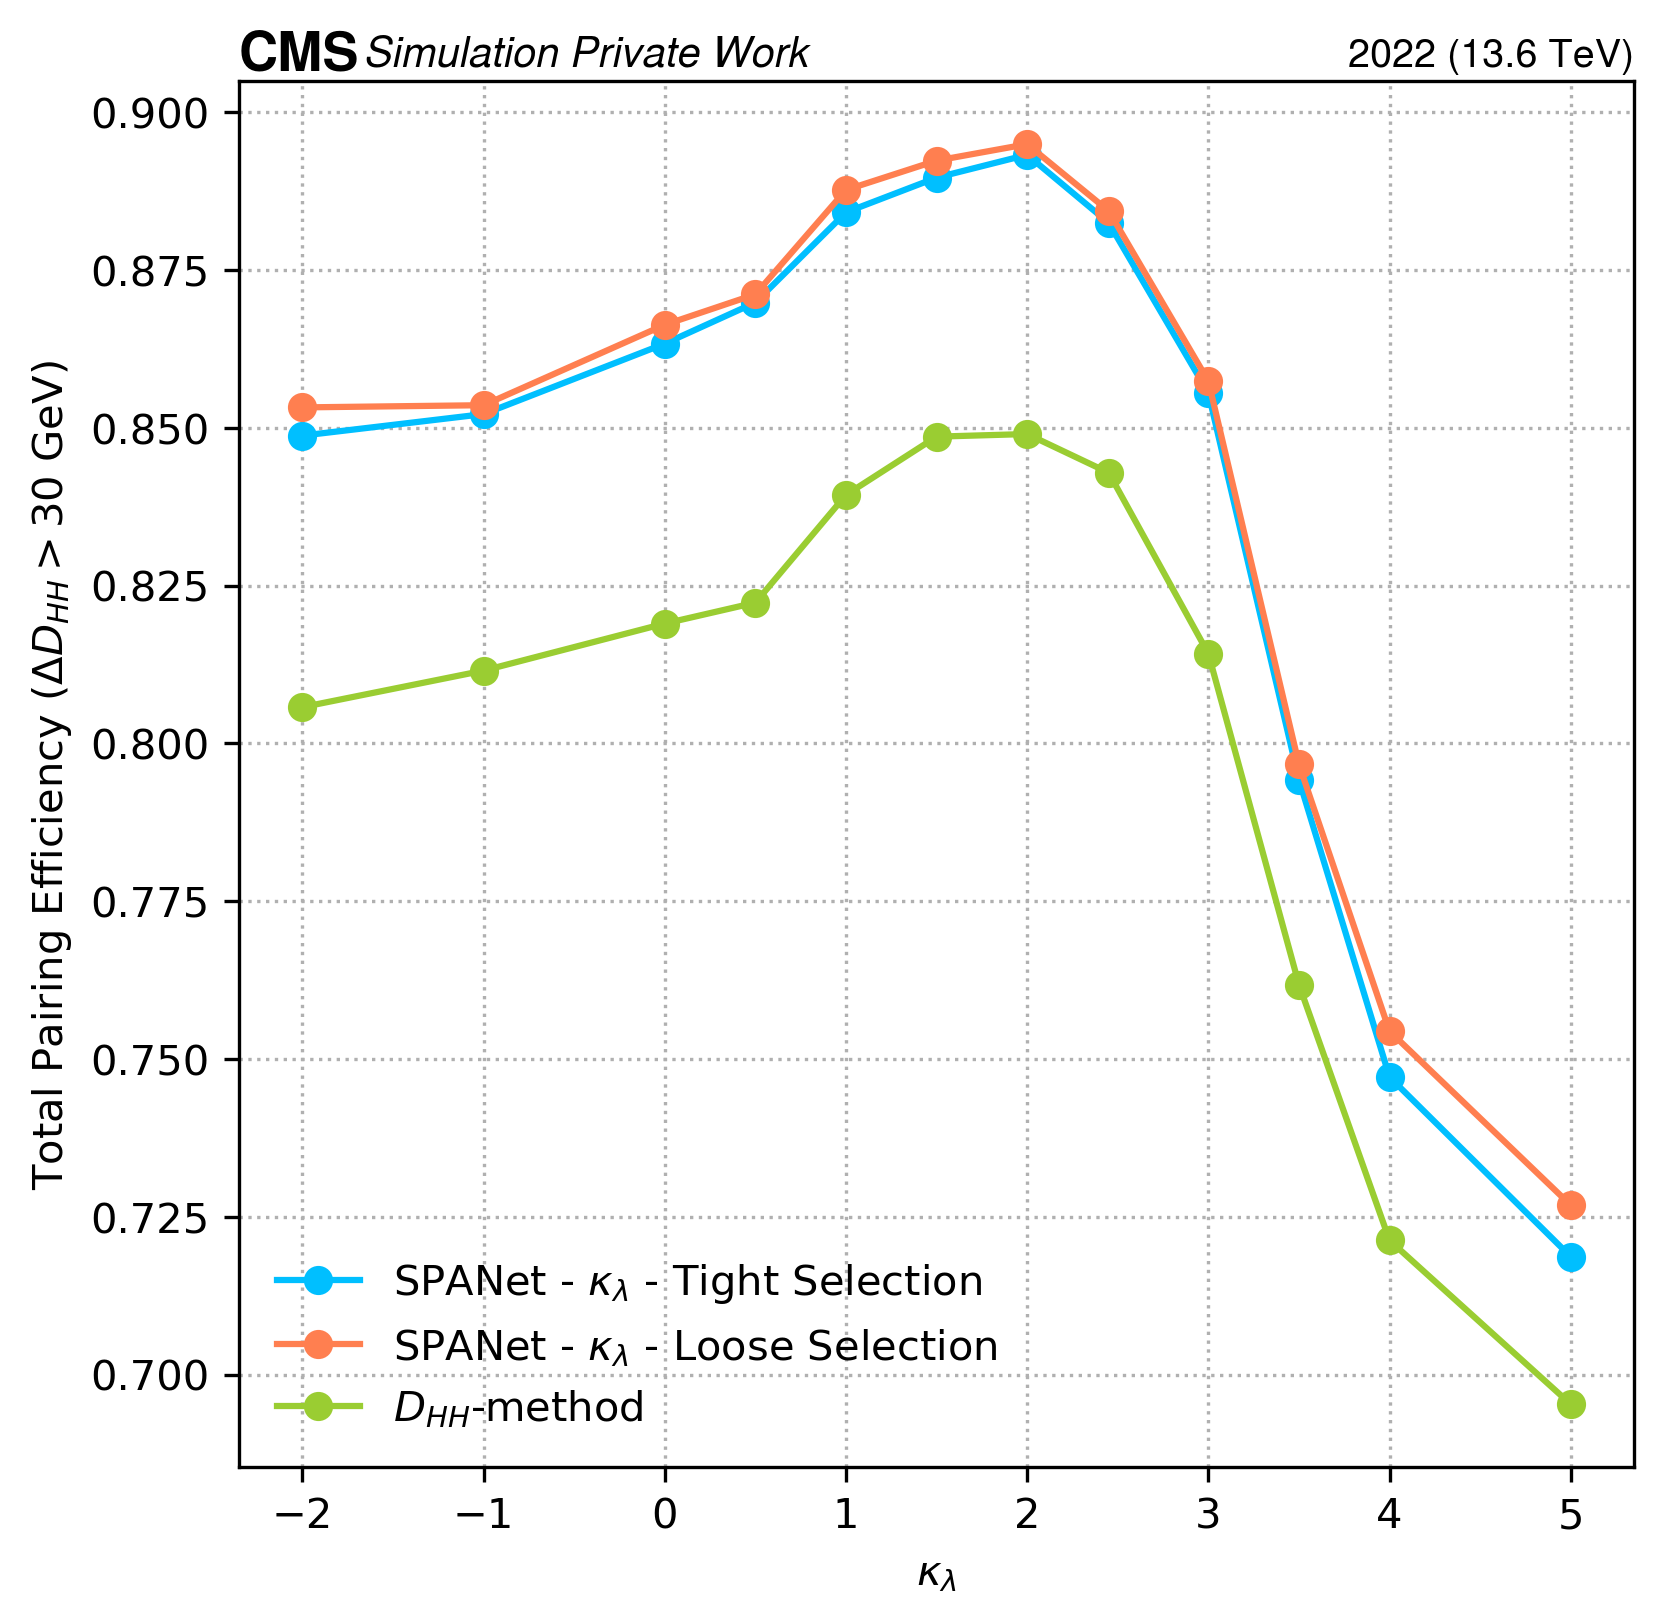
\includegraphics[width=0.6\linewidth]{Images/6.Improving/kappa lambda/loose vs tight.png}
    \caption{Comparison of trainings using Loose or Tight cuts presented in Table \ref{table:kl loose vs tight}). These trainings are compared to the $D_{HH}$-method used in Run 2.}
    \label{fig: loose vd tight}
\end{figure}

\begin{figure}[hbt]
    \centering
    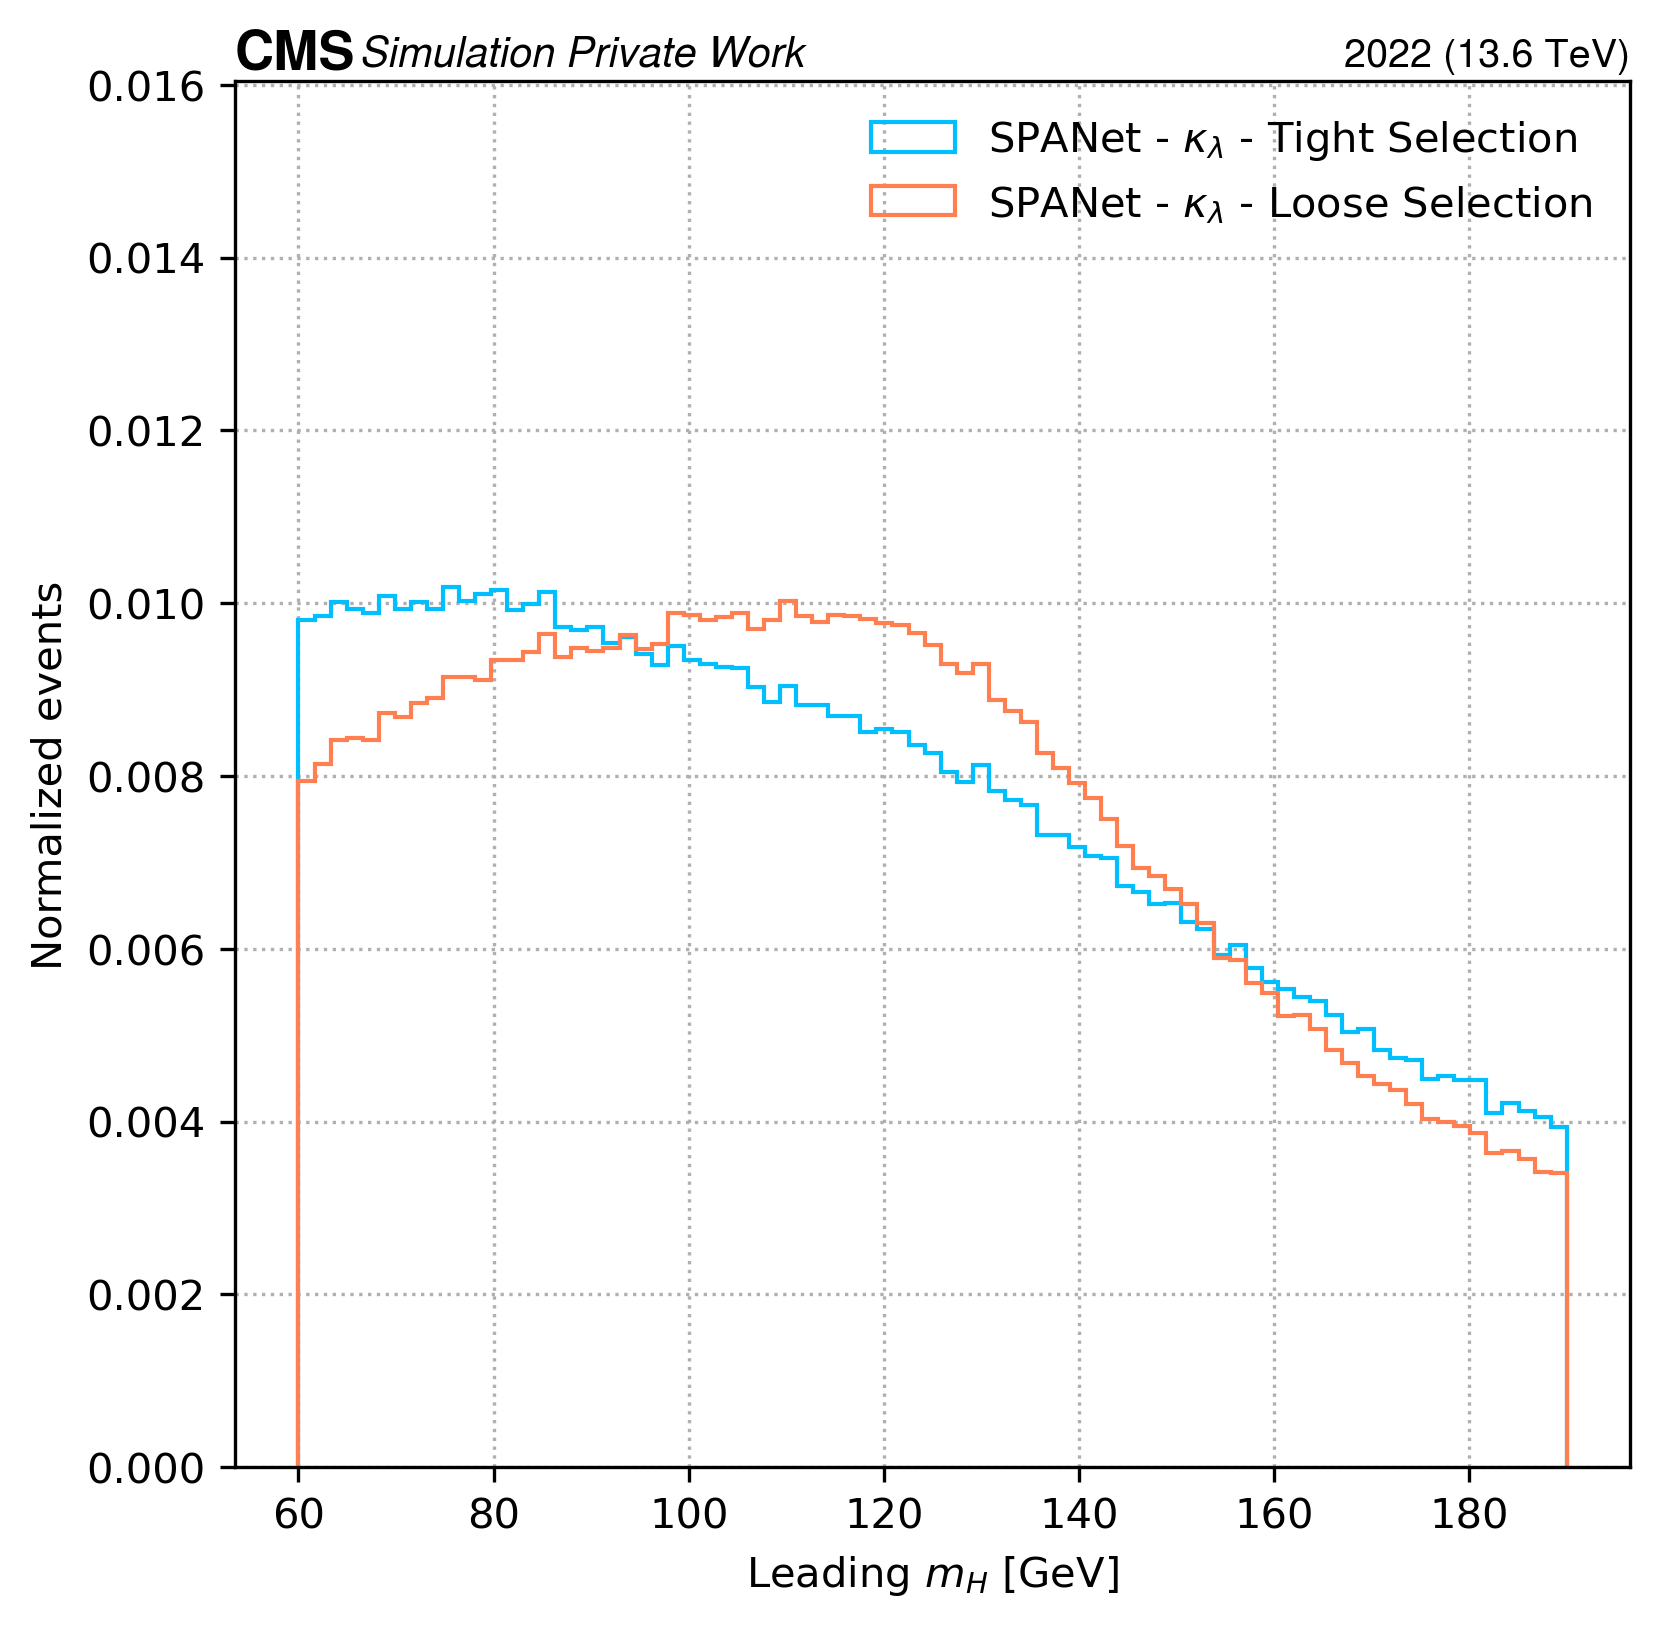
\includegraphics[width=0.6\linewidth]{Images/6.Improving/kappa lambda/leading h mass sculp.png}
    \caption{Distribution of the leading Higgs mass after evaluating the models presented in Table \ref{table:kl loose vs tight} on 2b data}
    \label{fig: leading H mass dist}
\end{figure}

\begin{figure}[hbt]
    \centering
    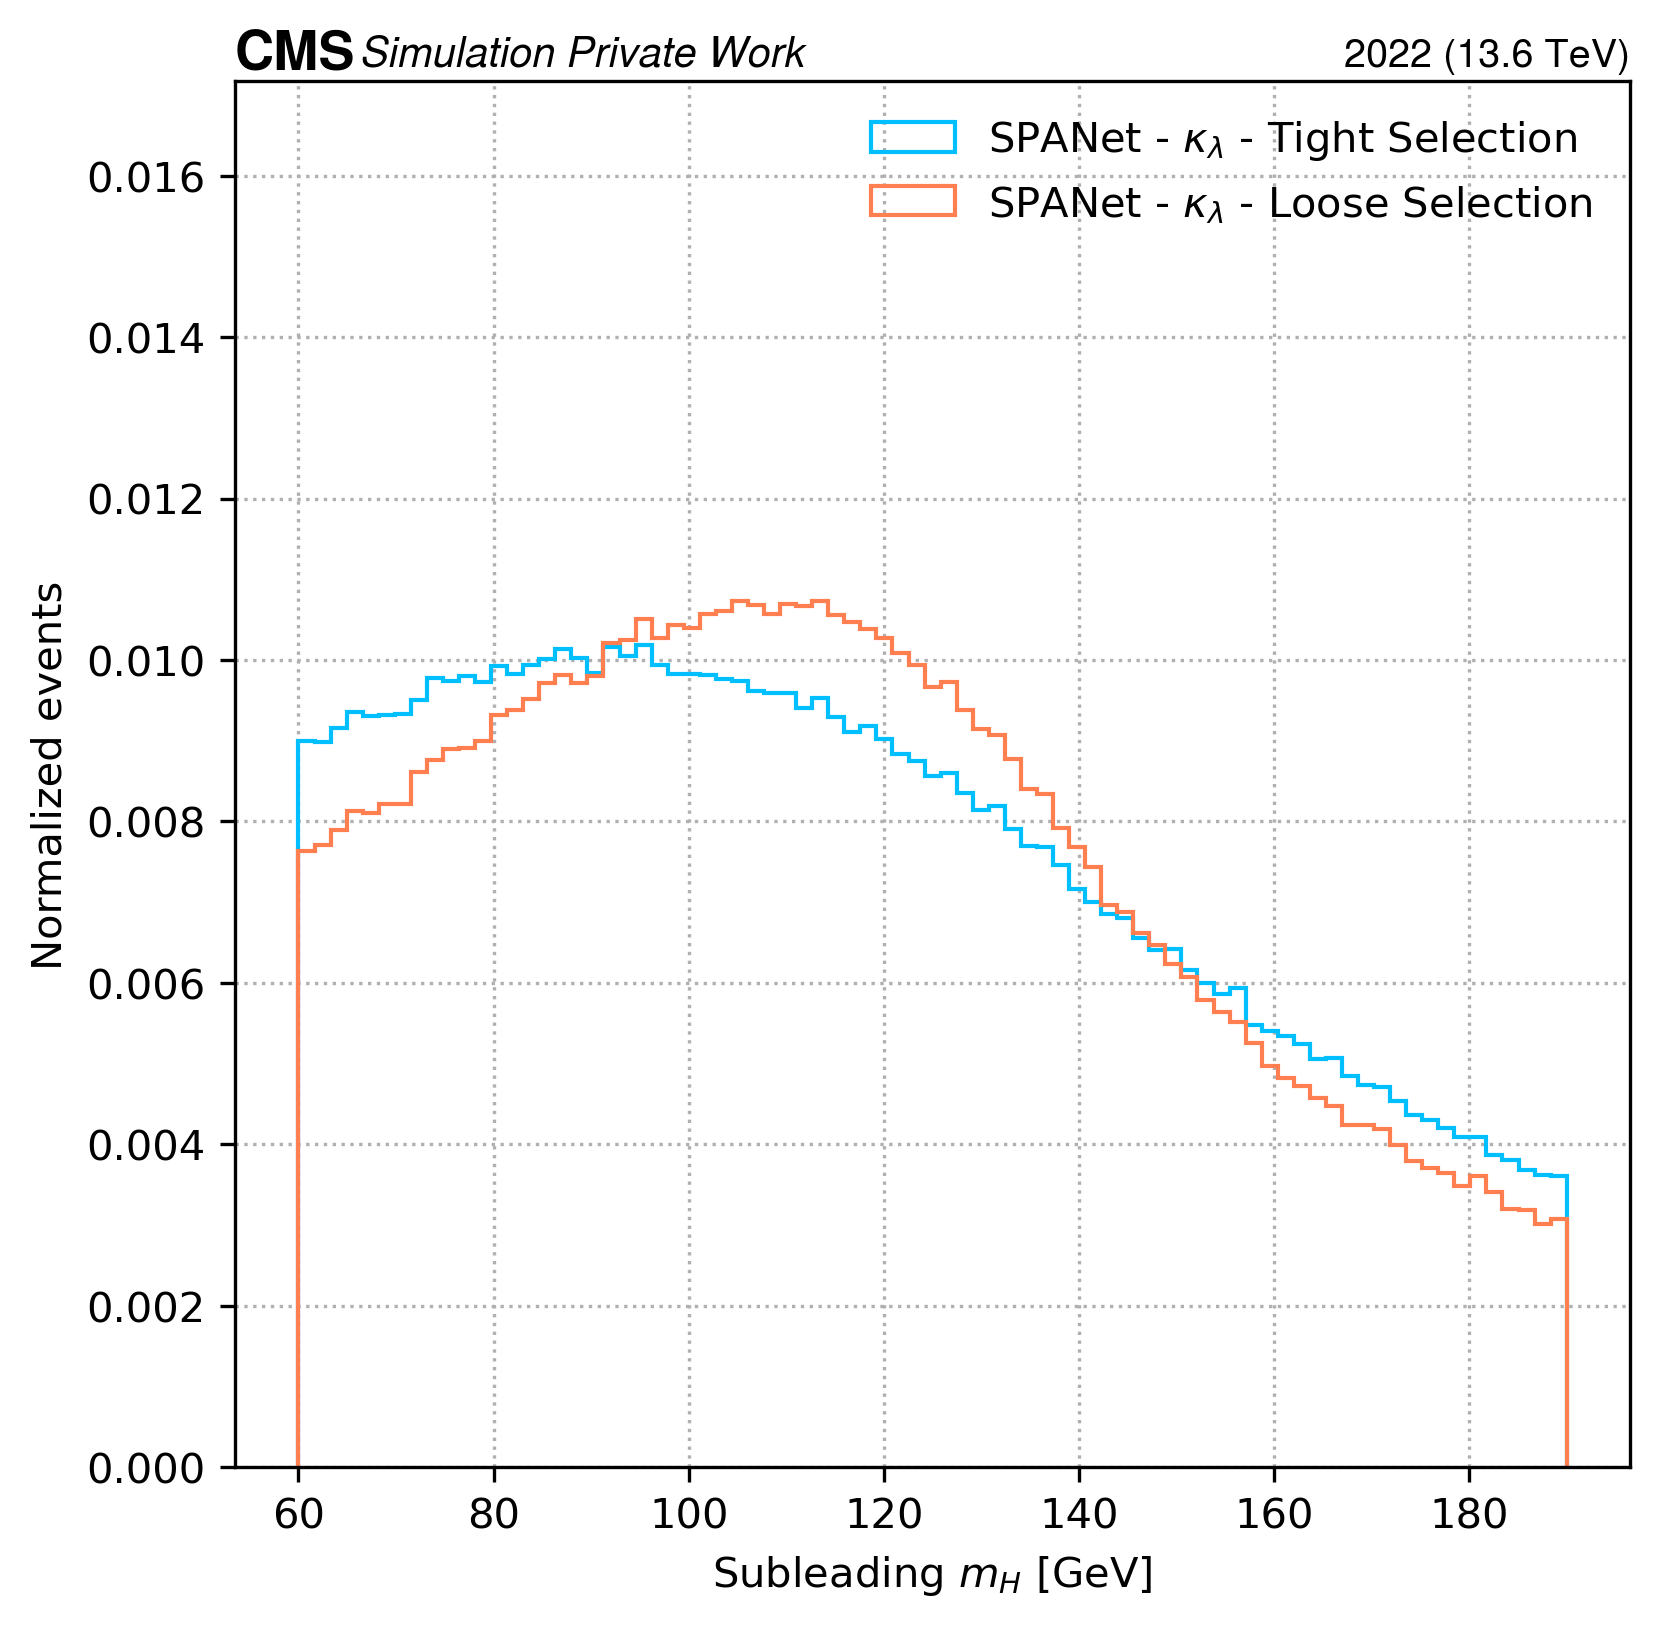
\includegraphics[width=0.6\linewidth]{Images/6.Improving/kappa lambda/sub leading H mass sculpt.png}
    \caption{Distribution of the subleading Higgs mass after evaluating the models presented in Table \ref{table:kl loose vs tight} on 2b data}
    \label{fig: subleading H mass dist}
\end{figure}

\newpage

\subsection{The final configuration} \label{subsection: Optimal config}
After comparing several configurations, we conclude that the best performance for jet pairing is given by the SPANet - \kl - Tight selection model which uses 5 jets as sequential inputs (with \pt reg, $\eta$, $\phi$ and b-tag), no explicit \kl input as global variable as well as the hyperparameters of the stable model shown in Table \ref{table: stable model}.
Figure \ref{fig: 2D mass dist kl} shows the 2D mass sculpting of the background. We do not observe any excess of events (background sculpting) in the SR.

\begin{figure}
    \centering
    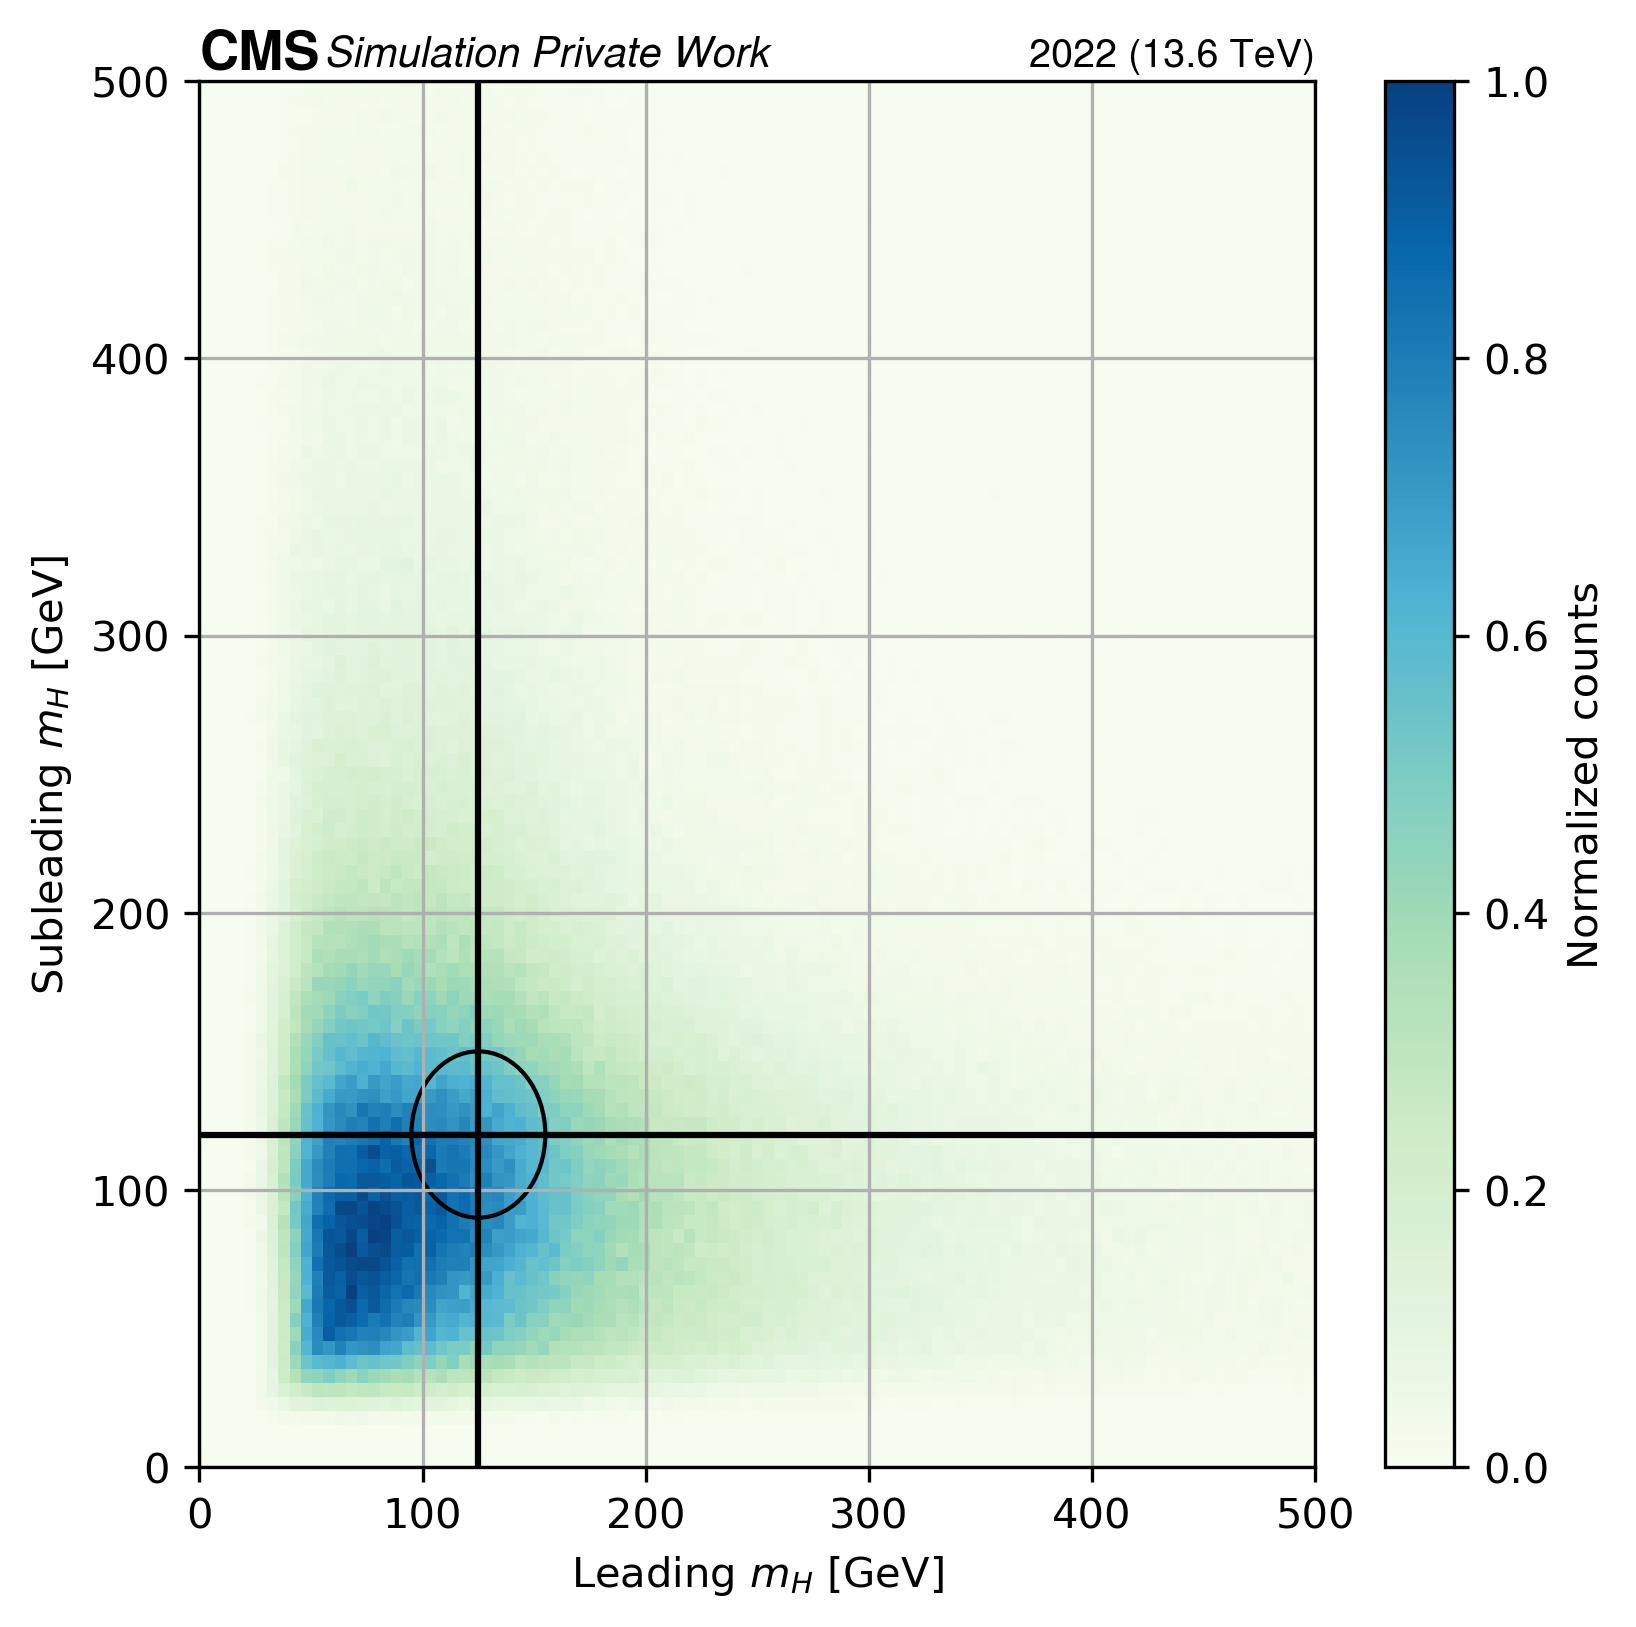
\includegraphics[width=0.6\linewidth]{Images/6.Improving/kappa lambda/mass dist best model.png}
    \caption{Higgs mass distribution of the leading Higgs on the x-axes and the subleading Higgs on the y-axes after the evaluation of  SPANet - \kl - Tight selection model on 2b data. The vertical black line corresponds to the mass of the leading Higgs and the horizontal of the subleading Higgs. The black circle defines the SR area defined in section \ref{section: HH4b}}
    \label{fig: 2D mass dist kl}
\end{figure}

% jets as inputs, pt reg, lite and stable model, tight cuts, no kl as inout explicitely